% \begin{savequote}[8cm]
% Alles Gescheite ist schon gedacht worden.\\
% Man muss nur versuchen, es noch einmal zu denken.

% All intelligent thoughts have already been thought;\\
% what is necessary is only to try to think them again.
%   \qauthor{--- Johann Wolfgang von Goethe \cite{von_goethe_wilhelm_1829}}
% \end{savequote}

\chapter{\label{ch:spf}A Possibility Frontier Approach to Diverse Talent Selection}\blfootnote{This chapter is based on two papers showcasing research done in concert with Kadeem Noray. Both contributed equally to the research. One paper is currently under review as: Kadeem Noray and Neil Natarajan. 2024. “Selecting for Diverse Talent: Theory and Evidence.” Under review at Economics of Talent Meeting, Fall 2024. The other is being prepared for submission as: Neil Natarajan and Kadeem Noray. 2024. “SPF: A Technology Probe Examining Diversity in Selection Processes.”. This version of the work is intended for publication to an economics audience; thus, this Chatper's writing style strays from the norms governing Chapters \ref{ch:xai}, \ref{ch:genai}, and \ref{ch:diversity}.}

\minitoc
% To-do:
% Relation to HCI – “Not fully trusting the user’s surface level intuitions is a key part of HCI research”
% Motivate this with “we did our homework, now we understand it, we need to go work with people”
% Make clear throughout that this chapter is a dialogue between researchers and program

\section{Motivation}
Chapter \ref{ch:diversity} designs six prototypes in cooperation with Rise and Ellison Scholars selectors. We ultimately find practitioner interest in all of these design prototypes. However, we warn as early as Chapter \ref{ch:context} of the dangers of placating subjective practitioner feedback in place of evaluating impact on decision-making. (This, in fact, is the very same issue with explainable AI we find in Chapter \ref{ch:xai}.) Thus, this chapter implements Prototype \ref{fig:diversity} in a field deployment with the Rise program to gain a more objective evaluation of its impact on decision-making.

\section{Introduction}\label{sec:spfintro}
% to-do: mention maybe that we've avoided implementing individual-level stuff because of the potential for automation bias.

The rise of diversity, equity, and inclusion initiatives suggests that various organisations (e.g. schools, firms, social impact programs, etc.) are genuinely interested in selecting for diverse talent. This is driven, at least in part, by recent declines in discrimination \cite{hsieh2019allocation}, increases in the perceived return to diversity \cite{deming2017growing, page_diversity_2017, noray2023systemic}, and increased social pressure for demographic representation \cite{minkin2023diversity}. In this chapter, we deploy technology based on Prototype \ref{fig:diversity} in a field study with Rise. We seek to understand whether this technology can help organisations select more diverse and talented cohorts.\footnote{Throughout the chapter, we use ``talent'', ``aptitude'', and ``performance'' interchangeably. In doing this, we recognise that organisations generally seek to optimise for talent or aptitude, but do so via measurements of applicant performance on assessments or assignments. In practice, this process carries its own risks; e.g., heterogenous biases in metrics or assessment methods will lead some subgroups to appear less talented or apt than others, even when no true difference in talent or aptitude exists. On the whole, this chapter is more interested in measurements of diversity than of talent or aptitude; thus, while these risks are of crucial importance to fair selection processes, they are tangential to the focus of this chapter.}

In order to assess this technology's usefulness, we begin by developing a simple model of cohort selection. Organisations receive $N$ applications and must select $n<N$ individuals to construct a cohort from the total set of potential cohorts, each of which is indexed by $c$. The organisation seeks to maximize a preference function that is increasing in both a cohort's talent (e.g., the mean performance on an ability measure) and a cohort's diversity (e.g., an inverse distance to a set of target proportions of demographic groups). This simultaneous optimisiation problem yields a frontier, which we term the Selection Possibility Frontier (SPF). The SPF represents the set of non-dominated cohorts, i.e., the set of cohorts that are not outperformed by any other cohort on both talent and diversity. We then use the SPF to implement Prototype \ref{fig:diversity} in the field, noting that a calculation or approximation of the SPF serves to produce the exact figure shown in Prototype \ref{fig:diversity}; we opt for a simple greedy estimation algorithm that relies on the submodularity, monotonicity, and non-negativity of diversity functions \cite{krause2014submodular, huppenkothen2020entrofy}.

Next, we turn to the empirical component of the chapter where we work with the Rise team to deploy this technology in Rise Cycle 2023 selection. We find that, in Cycle 2021, the set of finalists could have been $18.5\%$ more diverse without any reduction in performance, or $17.8\%$ higher-performing without any reduction in diversity. Similarly, in Cycle 2022, the finalists could have been $14.6\%$ more diverse without any reduction in performance, or $24.1\%$ higher-performing without any reduction in diversity. This indicates that, in the absence of our Decision-Support Tool (DST), Rise selects cohorts well within the frontier; i.e., both cohorts chosen were non-first-best as measured by the program's definitions of diversity and performance. We also show that, when the program was given access to the SPF in Cycle 2023, they significantly improved the efficiency of their selection process, choosing a cohort that was more diverse, higher performing, and very near to the estimated SPF. This suggests that the DST aided their decision-making and allowed them to better optimise in the face of a complex choice.

Though encouraging that the technology deployed in this Chapter improves organisational selection, we still require an understanding of why. In seeking to understand why programs do not simply select on the frontier without support, we prove that this problem, though simple to state, is computationally complex. This is for two intuitive reasons. First, an individual's contribution to the diversity of the cohort depends on who else will be part of the cohort. Thus, to determine which cohort is the smallest distance from the predefined "ideal" diverse cohort, every possible cohort needs to be assessed. Second, when diversity preferences are for representation of at least two non-mutually exclusive identities (e.g. ethnic minorities and women), optimally selecting members of one group constrains your ability to do the same for the other group. Formally, we show that maximizing functions on subsets is in general non-polynomial. We then show that, when we restrict our attention to functions formalizing diversity as organisations measure it, the `Vertex Cover' problem, known to be $\mathbf{NP}$-hard, reduces to diversity maximization. This implies that calculating the maximal diversity conditional on cohort performance (what we refer to as the Selection Possibilities Frontier, or SPF) is also $\mathbf{NP}$-hard. Selecting on the SPF, then, is likely prohibitively costly for many organisations.

To account for this complexity, we augment our model of cohort selection by forcing organisations to incur a computational marginal cost for each unit of increased cohort diversity. This represents the fact that, to find a more diverse cohort, one must engage in the laborious process of composing potential cohorts and comparing them. This is in sharp contrast to finding more talented cohorts, which is comparatively simple -- and, therefore, modeled as costless -- because each individual's contribution to cohort talent is unrelated to the remainder of the cohort. This updated model appears to better describe organisational behaviour. This has two implications: (1) organisations will tend to select sub-optimal (i.e. non-first-best) cohorts and (2) organisations will improve on both performance and diversity if the gain access to a technology that reduces this computational marginal cost. 

As an aside, we use our SPF estimation procedure to evaluate the efficacy of alternative screening and selection methods. To do this, we leverage two unique aspects of the program. First, the program collects both traditional merit-based measures -- including cognitive tests, written essays, and referring organisations -- as well as non-traditional measures -- including peer reviewed video essays, gamified skill tests, and application platform behaviors. Second, the program engaged in effectively no screening before receiving concrete projects from applicants, making it possible to estimate valid counterfactual diversity and performance of cohorts had they been screened in different ways. Leveraging these features, we find three key results. First, selecting only on the basis of cognitive ability or traditional metrics would have improved cohort performance relative to random selection, but would significantly restricted the program from reaching its diversity goals. By contrast, selecting only on peer reviews performs similarly on performance but improves diversity substantially. Second, all alternative selection methods we explore result in selecting cohorts well within the SPF and, therefore, leave substantial diversity and performance gains on the table. And third, the trade-off implied by the SPF between talent and diversity is steeper if traditional measures are used to measure talent than if applicant projects are used. 

\section{Related Work}\label{sec:spfrelwork}
This chapter contributes to a growing economics literature studying the influence and potential of algorithms. Most research in this area has focused on measuring the effects of AI tools both at the economy-wide (`macro') level \cite{acemoglu2022automation,babina2024artificial,calvino2023portrait,zolas2021advanced,webb2019impact} and in more specific (`micro') contexts like bail decisions and radiology \cite{albright2023hidden,kleinberg2015prediction,stevenson2019algorithmic,angelova2023algorithmic,imai2023experimental,grimon2022impact,noy2023experimental,brynjolfsson2023generative,bundorf2019humans, mullainathan2019machine, ribers2020machine, agarwal2023combining}. This chapter is more closely related to the small subset of this work that \emph{develops} AI tools to improve or assess human problem-solving in some respect.\footnote{Though small in economics, there is a larger literature in computer science that focuses on developing algorithmic tools to replace or improve humans' capacity to solve problems. Most closely related to this chapter are machine systems that help organisations select in ways that are `unbiased' \cite{tambe2019artificial,raghavan2020mitigating} or account for `diversity' \cite{gillet_diversity_2011,huppenkothen2020entrofy}. Our chapter differs from these because we account for trade-offs between diversity and other desiderata (e.g. talent, productivity, etc.).}  This includes work that develops methods to compare the efficacy of human vs. AI predictions \cite{kleinberg2018human,rambachan2024identifying} and several papers that develop algorithms specifically to improve the selection or assignment of personnel \cite{li2020hiring,bergman2021seven,kleinberg2018algorithmic,huppenkothen2020entrofy}. This chapter contributes to this literature by developing and applying algorithmic tools to the increasingly relevant diverse talent selection problem. 

This chapter is closely related to \textcite{kleinberg2018algorithmic}, which introduces an algorithm that colleges can use to calculate the most meritorious cohort at any threshold of representation for a single underrepresented group. Their algorithm is straightforward: define a minority group (e.g. black applicants) and the corresponding majority group (e.g. white applicants), rank applicants within each group by measure of merit (e.g. test scores, predicted college performance, etc.), set a threshold for the proportion of those selected who should be part of the minority group, select minority group members from the highest ranking down until the threshold is met, and finally, select the majority group members from the highest ranking down until all slots are filled. Though effective, this procedure only works when the organisation aims to represent mutually exclusive minority groups. If diversity preferences are instead for representation of multiple non-mutually exclusive groups (e.g., female applicants and black applicants), this strategy no longer works. This chapter relaxes this assumption and outlines the conditions under which the diversity-performance frontier can be estimated regardless of the number or type of identity characteristics organisations seek to represent.

This chapter is also related to the growing economics literature on the impact of new screening technologies on the productivity and diversity of the personnel that organisations select. An early paper on this topic is \textcite{autor2008does}, which shows that adding personality tests to the job applicant screening process in a national retail firm increased the productivity of selected workers without reducing minority representation among hires. More recently, \textcite{li2020hiring} demonstrate that, within a Fortune 500 tech company, diversity and productivity of hires can be improved by using exploration-based applicant screening algorithms that recommend applicants with rare sets of characteristics at higher rates in order to improve noisy predictions and, therefore, learn how to find promising applicants from atypical backgrounds. Similarly, \textcite{bergman2021seven} show that, across seven colleges, using a prediction algorithm instead of a test to decide whether to place students into remedial classes improves student performance and increases minority representation in college-level (non-remedial) courses. This chapter adds to this literature in two ways. First, rather than focusing on comparing a new screening method to the status quo, this chapter develops a procedure for estimating the diversity-performance frontier itself. Second, leveraging the novel design of the scholarship's application process in combination with our estimate of the SPF, we provide new evidence on the efficacy of screening on traditional "merit" measures. 

This chapter is also related to work across fields defining fairness and equity in talent selection. Much of this work builds on the \emph{similar treatment principle} whereby individuals who perform similarly on some dimension(s) are treated equally in selection \cite{dwork_fairness_2012}.\footnote{Though not generally mentioned in this literature, the similar treatment principle is the normative basis on which differential treatment of demographic groups in audit studies is deemed wrong.} This approach has been criticized, however, on the grounds that in circumstances when performance and demographic factors are correlated, employing this principle could substantially reduce the diversity of the chosen cohort, which may not accord with a decision-makers fairness preferences \cite{fleisher_whats_nodate}. Furthermore, when measurements of performance are biased in favor of certain demographic groups, similar treatment on the basis of these measurements leads to applicants with the same underlying ability being treated differently \cite{fleisher_whats_nodate}. An alternative perspective is to assume fairness and equity are captured by diversity, and instead to measure diversity directly. Three measures are commonly considered: (1) the majority-minority approach, (2) the generalized variance approach, and (3) the entropy statistic (see \textcite{budescu2012measure} for a summary). Following \textcite{huppenkothen2020entrofy}, we measure diversity using an entropy-based approach. We do this for two reasons. First, as \textcite{huppenkothen2020entrofy} demonstrate, versions of an entropic scoring function have mathematical properties (i.e. submodularity and monotonicity) that allow us to both easily estimate the SPF and to bound the error of our estimates. Second, preferences for diversity often take the form of ``closeness to a proportional target for each relevant identity characteristic'', which can be represented easily using entropic functions. Thus, our work adds to the applications of entropy-based methods for measuring diversity.

\section{Theory and Methods}\label{sec:spfmethod}
\subsection{Evaluating Organisational Decision-Making}\label{ssec:measurement}
Central to this chapter is the desire to evaluate Prototype \ref{fig:diversity} on real results, rather than satisfaction. However, there is no ground truth of decision-making in the scholarship program. Thus, we define a model of talent selection and use this model in assessing a field deployment of the prototype. This model relies on a key object, the Selection Possibilities Frontier (SPF), to bound the range of possible cohort selections on two axes: average applicant performance on individualised metrics of talent, and overall group diversity. With this model, we can evaluate the program's decisions in terms of their proximity to the SPF; the closer a program is to the SPF, the more efficient their selection process. In this case, we deploy Prototype \ref{fig:diversity} with Rise; their metrics for talent and diversity can be found in Appendix \ref{app:programs}.

We start by considering a simple version of the organisation's optimisation problem. Organisations receive $N$ applications and must select $n<N$ individuals to form a cohort $c$ from the set of all potential cohorts $C$. The organisation prefers both that the selected cohort is higher performing on some measure of talent and more diverse. For now, a cohort's diversity can be thought of as the inverse of a multidimensional measure of distance between the set of proportions of the cohort who belong to key demographic groups and a set of target proportions the organisation has for each group (we discuss definitions of diversity in more detail in Section \ref{subsec:dts_nphard}). If we let the performance and diversity of a given cohort $c$ be given by the functions $P(c)$ and $D(c)$, respectively, then the above description is equivalent to letting the organisation's preference function $F\Big(D(c),P(c)\Big)$ exhibit $F_D>0$, $F_P>0$, and $F_{DP}\geq0$, where subscripts indicate partial derivatives with respect to the variable in the subscript. 

Conceptually, this would represent a scenario where an organisation can observe $D$ and $P$ for every possible cohort and simply select the one that maximizes $F(D,P)$. If we assume the organisation behaves rationally, we know the organisation will not choose dominated cohorts. Formally, $c^*$ can be the optimal cohort if and only if there exists no $c'$ such that $D(c')>D(c^*)$ and $P(c')\geq P(c^*)$ and there exists no $c'$ such that $D(c')\geq D(c^*)$ and $P(c')> P(c^*)$. We know that the optimal cohort must be in the set of non-dominated cohorts which we define as the Selection Possibilities Frontier (SPF). If we assume, for expositional purposes, that the SPF is continuous, we can represent it as the following function:

\begin{equation}
G(p) := \max\Big[D(c)|P(c) \geq p\Big]
\end{equation}

\noindent In words, $G(p)$ merely gives the highest possible diversity for every cohort performance level. The diverse talent selection problem, then, can be represented as choosing a cohort to maximize $F$ subject to a constraint that the choice be on the SPF. Formally, 

\begin{equation}
\max_{d,p} F\Big(d,p\Big) \text{ \bf{ s.t. } } d = G(p), \nonumber 
\end{equation}

\noindent which is equivalent to

\begin{equation}
\max_{p} F\Big(G(p) ,p\Big). \label{eq:selection_simple}
\end{equation}

The solution to this simple version of the model is depicted in Figure \ref{fig:model_spf}. Notably, this model suggests that organisations should always select cohorts on the frontier, as all cohorts within the frontier are dominated by cohorts that are either least as diverse and more talented or at least as talented and more diverse.

\begin{figure}[htbp]
    \centering
    \caption{This figure depicts an example solution to an iteration of the selection problem, which is described in Equation \ref{eq:selection_simple}. The solid blue curve represents the Selection Possibilities Frontier (SPF), the dotted blue curve represents the organisations indifference curve corresponding to the highest achievable utility, and the blue dot represents the diversity and performance of the optimal choice (i.e. the first-best solution). }
    \label{fig:model_spf}
    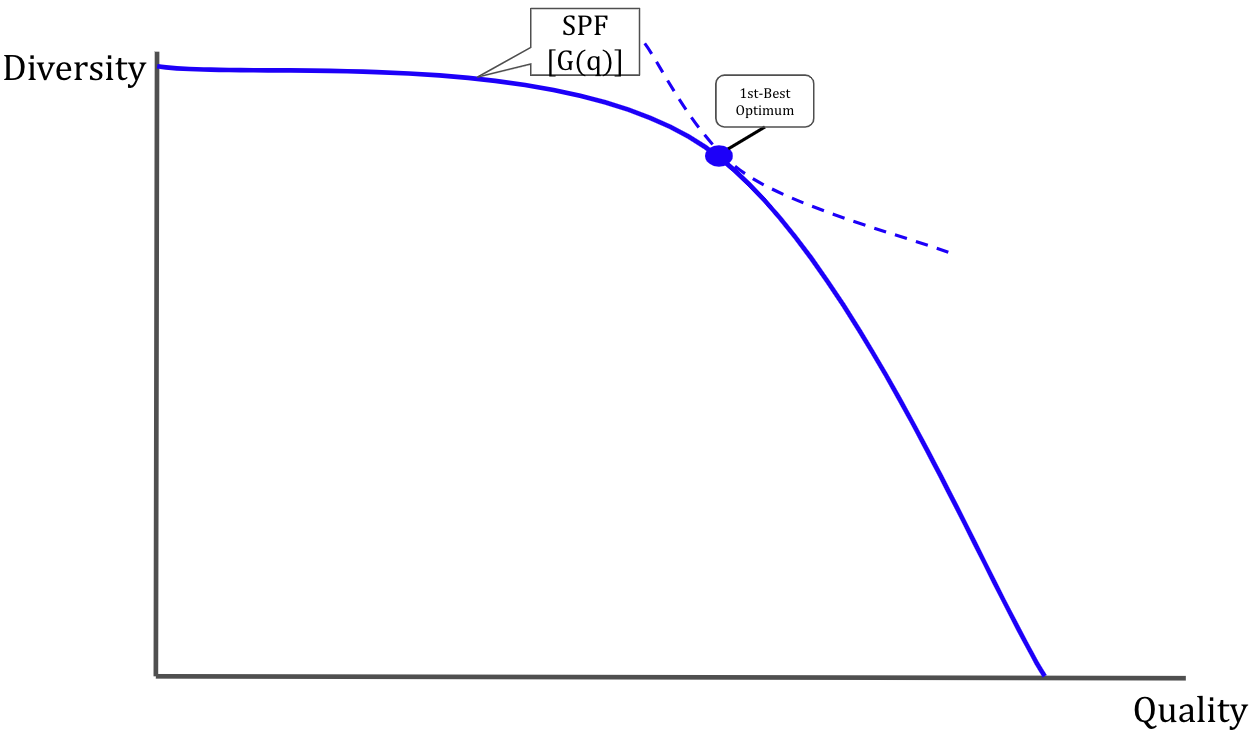
\includegraphics[width=\textwidth]{spf/model_spf.png} 
\end{figure}

\subsection{Defining the Classes of Diversity and Performance Functions}\label{subsubsec:div_talent_def}
Without knowledge of the types of functions $D(c)$ and $P(c)$, Equation \ref{eq:selection_simple} proves difficult to instrument in practice. In this section, we define the classes of functions $D(c)$ and $P(c)$ that are relevant for the diverse talent selection problem. In particular, we will formalise \emph{proportional diversity} and \emph{count diversity} as kinds of diversity, and assume performance to be a real-valued individual-level metric, aggregated by summation.

In both cases, here, we work with Rise to identify their preferences w.r.t. different kinds of diversity and performance. We then implement their preferences as functions $D(c)$ and $P(c)$.

\paragraph{Proportional diversity} When organisations they make statements like: ``we desire at least $x$ percent of group $g$'', they are speaking of proportional diversity. But, since organisations aim to select cohorts of a specific size, we can reframe this goal as ``we desire at least $x*n$ individuals from group $g$", where $n$ is the total number of applicants in the cohort.\footnote{This reframing will turn out to be helpful in Section \ref{sec:spf_alg} when we develop our SPF estimation strategy} If we let $\chi_g(c)$ be the proportion of $c$ in group $g$ and $\sigma_g(c)$ bne the total number of applicants in $c$ who are in group $g$ This can be formalised into the proportional diversity function:

\begin{equation}
    \begin{split}
        \delta_{g}^{prop}(c,x) &:= n*\min(\chi_g(c), x) \\
        & := \frac{n* \min(\sigma_g(c), x*n)}{n} \\ 
        & := \min(\sigma_g(c), x*n). \label{eq:prop_div_function}
    \end{split}
\end{equation}

If, for example, an organisation selecting 100 applicants would like their organisation to be least $40\%$ female the proportional diversity function associated with this goal is $\delta_{female}^p(c, 40) := \min(\vec{\mathbf{f}}*\vec{\mathbf{c}}, 40)$ where $\vec{\mathbf{f}}$ is a Boolean vector indicating which applicants are female and $\vec{\mathbf{c}}$ is a Boolean vector that indicating who is in cohort $c$. This can be thought of as an inverse distance along the dimension of group representation between cohort $c$ and an ideal cohort $c^*$ where $\sigma_g(c^*) = x*n$.

\paragraph{Count Diversity} The second common type of diversity is what we call \emph{Count diversity}. This formalises organisational statements like: ``we desire at least one person from $m$ groups''. To formalise this notion, let $\mathbb{I}(\cdot)$ be an indicator function that is equal to 1 if the condition within is true. We can now represent a count diversity preference as:

\begin{equation} 
    \begin{split}
        \delta_G^{count}(c,m) &:= \min\big(\sum_{g \in G}\mathbb{I}(\sigma_g(c)\geq 1), m\big), \label{eq:count_div_function}
    \end{split}
\end{equation}

\noindent where $G$ is the set of relevant groups the organisation wants represented by at least a single individual. This type of function is ideal for representing geographic representation goals where educational institutions, like colleges or scholarships, often have goals like ``we want a student from every state'' or ``we want as many countries as possible represented''. 

\paragraph{Overall Diversity} Ultimately, organisations care about all of their diversity goals, not just one. Thus, the diversity functions that are relevant for an organisation must be aggregated if we want to formalise an organisation's overall preference for diversity. We define this aggregation as an organisation's diversity score $D(c)$, which generally has the following form: 

\begin{equation}
A\big(\delta_{g_1}^{prop}(c,x_1),...,\delta_{g_K}^{prop}(c,x_K),\delta_{G_1}^{count}(c, m_1),...,\delta_{G_J}^{count}(c, m_J)\big), \nonumber
\end{equation}

\noindent where $A(\cdot)$ is an aggregator function. It is essential that $D(c)$ increases as a cohort gets ``closer" to one of the underlying diversity goals because this is sufficient to identify cases when one cohort dominates another, even if the formalization misses something subtle or difficult to articulate about the organisation's diversity preferences. A flexible but simple aggregator function is a weighted sum, where organisations can place different emphasis on each of the goals. So, for the remainder of this chapter, we use diversity scores of the following form: 

\begin{equation}\label{eq:d_equation}
D(c,\vec{\mathbf{w}},\vec{\mathbf{x}},\vec{\mathbf{m}}, \vec{\mathbf{g}}, \vec{\mathbf{G}}) := \sum_{k\in K}w_k\delta_{g_k}^{prop}(c,x_k) + \sum_{j \in J}w_j\delta_{G_j}^{count}(c, m_j),
\end{equation}

\noindent where $\vec{\mathbf{w}},\vec{\mathbf{x}}, \vec{\mathbf{m}}, \vec{\mathbf{g}}, \vec{\mathbf{G}}$ are vectors of the organisation's weights, proportional targets, count targets, groups of interest to proportional diversity functions, and sets of groups of interest to count diversity functions, respectively.\footnote{Another attractive option is a CES aggregator because it allows for specifying degree of substitutability between diversity goals, but this comes at the cost that many organisations don't really know this (introducing similar problems as requiring goals at the mutually exclusive group level). Nonetheless, the authors are currently working on establishing whether the estimation procedure presented in Section \ref{sec:spf_alg} is viable for a CES aggregator.} In general, we suppress the vector notation opting to refer to the diversity score as $D(c)$ where this doesn't lead to confusion.

\paragraph{Talent, Aptitude, or Performance} Relative to diversity, our definition of performance is simple. In general, organisations measure aptitude for their program using and individualised metric, usually performance on some assessment or assignment. Common examples include test scores, essays, or grades for educational organisations or technical interviews for tech hiring. More sophisticated (though uncommon) measures might be the predicted success of an individual based on a set of performance metrics. In this chapter we assume that organisations already possess a real-valued talent metric $\rho_i$ evaluated at an individual-level.\footnote{For details on Rise's talent metric, see Appendix \ref{app:programs}.} A cohort's \emph{talent}, then is defined as the sum of the talent level of the individual members, which is given by:

\begin{equation}
P(c) := \sum_{i \in I_c}\rho_i,
\end{equation}

\noindent where $I_c$ is the set of all individuals $i$ in cohort $c$. Unlike with diversity, $P(c)$ is straightforward because each individual's contribution is $\rho_i$ regardless of whoever else is in the cohort. Note that, so long as an organisation fixes their desired cohort size beforehand, optimising for the sum of $\rho_i$ is identical to optimising for mean $\rho_i$.

We represent an organisation's preference function $F$ as a weighted sum of performance and diversity functions. That is:

\begin{equation}\label{eq:f_spec}
F(D, P, c, \iota) := \iota*D(c)+(1-\iota)*P(c)
\end{equation}

\subsection{Implementing Prototype \ref{fig:diversity} in the Field}\label{sec:spf_alg}
As it happens, the SPF modelled in Figure \ref{fig:model_spf} can be used to implement Prototype \ref{fig:diversity} in the field. I.e., a calculation of the SPF using an organisation's preference function yields all of the data required to plot Prototype \ref{fig:diversity} (which is, as it happens, just a depiction of the SPF presented alongside contextual information designed to help selectors best understand the visualisation). However, as we will demonstrate in Theorem \ref{thm:specific-nphard}, calculating the SPF outright is unfeasible.\footnote{A keen reader may note that, under stricter conditions, others have already introduced algorithms for calculating the SPF outright. For example, \textcite{kleinberg2018algorithmic}'s algorithm can be easily extended to calculate the SPF when an organisation only possesses one proportional diversity preference.} Instead, we rely on a greedy algorithm to approximate the SPF.

Greedy optimisation is the practice of approximating an optimal solution to an iterative process by, at each iteration, making a choice that optimises the process at that iteration (i.e. ignoring iterations before and after) \cite{nemhauser1978analysis}. It is well known that greedy optimisation can be used to build near-optimal subsets of a given set when the objective function is non-negative, monotone, and submodular \cite{Feldman_Harshaw_Karbasi_2017,nemhauser1978analysis}. Though these conditions are not strictly necessary, results are not so clear when one of these conditions is dropped \cite{Feldman_Harshaw_Karbasi_2017}.

While non-negativity is self-explanatory (the objective function cannot be less than zero), monotonicity and submodularity deserve further clarification. In our context, monotonicity will require that cohorts are always more diverse than their smaller sub-cohorts while submodularity will require that an applicant's marginal effect on diversity for a cohort will be (weakly) less than her marginal effect on diversity for a smaller sub-cohort. More formally, a function $D$ defined on subsets of some universe $U$ is monotone if and only if 

\begin{equation}
    \label{eq:mononicity}
    \forall Y \subseteq U, X \subseteq Y: D(X)\leq D(Y),
\end{equation}

\noindent and is submodular if and only if

\begin{equation}
    \label{eq:submodularity}
    \forall Y \subseteq U, X \subseteq Y, x \in U \setminus Y: D(X \cup \{x\}) - D(X) \leq D(Y \cup \{x\}) - D(Y).
\end{equation}

This may appear constraining, but, luckily, both diversity functions $\delta_g^{prop}(c)$ and $\delta_G^{count}(c)$, $D(c)$,the talent function $P(c)$, and $F(D,P)$ all satisfy these conditions as defined in Section \ref{subsubsec:div_talent_def}. We show this in Theorems \ref{thm:submodularity_additive}, \ref{thm:monotonicity_additive} and \ref{thm:f_sub_mon} in Appendix \ref{app:spfmath}.

Now that we have established the necessary restrictions on functions $F(D,P)$, we present a greedy algorithm that finds $c$ so as to optimise $F(D, P, c, \iota)$; by repeating this for various values of $\iota$, we obtain the frontier between $D(c)$ and $P(c)$ (i.e., the SPF). This algorithm relies on two observations. First, any point on the SPF can be represented as the maximum of a weighted sum $f(\iota,c) = \iota*D(c) + (1-\iota)*P(c)$ where $\iota \in [0,1]$. Second, any $f(\iota,c)$ is monotonic and submodular. In this context, the algorithm repeatedly maximizes a weighted sum of diversity and talent, varying  the weight put on each element in each maximization. Formally, the algorithm maximizes $f(\iota,c)$ $m$ times, where each iteration optimises $\iota = \frac{m_i}{m}$. Then, for each $f$, this algorithm builds each cohort $c$ from $c$ of size $0$ until size $n$ by adding an applicant \textit{not} in the current cohort $c$ ($u \in U \setminus c$) that yields the highest $f$ value (i.e., that maximises $f(c \cup \{u\})$). This algorithm is presented more formally in Algorithm \ref{alg:frontier}. 

\begin{algorithm}
    \caption{Greedy Frontier Optimisation}\label{alg:frontier}
    \begin{algorithmic}
    \State \textbf{For} each desired point on the frontier defined by $\iota \in [0, 1]$
    \State \hspace{\algorithmicindent} \textbf{Let} $f_{\iota} := \iota*P+(1-\iota)*D$ be weighted average of $P$ and $D$
    \State \hspace{\algorithmicindent} \textbf{Begin} with empty cohort $c = \vec{\mathbf{0}}$
    \State \hspace{\algorithmicindent} \textbf{While} cohort $c$ is less than the desired size ($|c| < k$)
    \State \hspace{\algorithmicindent} \hspace{\algorithmicindent} \textbf{Find} applicant $i$ such that adding $i$ to $c$ maximizes $f_{\iota}(c + i)$
    \State \hspace{\algorithmicindent} \hspace{\algorithmicindent} $c := c + i$
    \end{algorithmic}
\end{algorithm}

It is well-known that the greedy algorithm yields a $\bigl( 1-\frac{1}{e} \bigr)$-approximation of any submodular, monotonic set function \cite{bordeaux_submodular_2014}. That is, the algorithm selects cohorts whose $f_\iota$ values are at least $\frac{1}{1-\frac{1}{e}}$ of the maximum $f_\iota$ any cohort of that size selected from the same applicant pool. For avoidance of doubt, a proof of these approximation bounds is presented in Theorems \ref{thm:greedy-approximation} in Appendix \ref{app:greedy-proof}. Thus, the Greedy Frontier Optimisation algorithm returns points on a curve that $\bigl( 1-\frac{1}{e} \bigr)$-approximates the true SPF\footnote{In practice, the outputs of the greedy algorithm do not always themselves form a convex curve. We remove produced points that do not sit on the convex curve.}. We note that this is a worst-case approximation ratio, and that the actual approximation ratio may be much better.

\section{A Field Study with Rise}\label{sec:spfresults}

We apply our methodology to evaluate our technology in a field deployment with Rise's Cycle 2023. Through this deployment, we document evidence that Rise selected finalists within the SPF -- consistent with the first prediction of our model -- and that Rise selected much closer to the SPF after they were given an SPF estimate to aid in selection of their third cohort.

\paragraph{Evaluating Past Selection Decisions} Before implementing our technology, we use the methodology described in Section \ref{ssec:measurement} to determine the efficiency of past selection decisions. In particular, we analyse the finalist selection portion of the 2021 and 2022 application cycles, where the program must construct a cohort of at most $500$ applicants from a pool of roughly $2000$. 

This analysis requires two steps: (1) applying Algorithm \ref{alg:frontier} to both cohorts to estimate the SPF and (2) comparing the actual talent and diversity levels of the finalist cohort to the estimated SPF. The model we developed in Section \ref{ssec:measurement} would suggest that this comparison should find that the chosen cohorts are on or near this frontier. 

\begin{figure}[htbp]
    \centering
    \begin{subfigure}[b]{0.4\textwidth}
        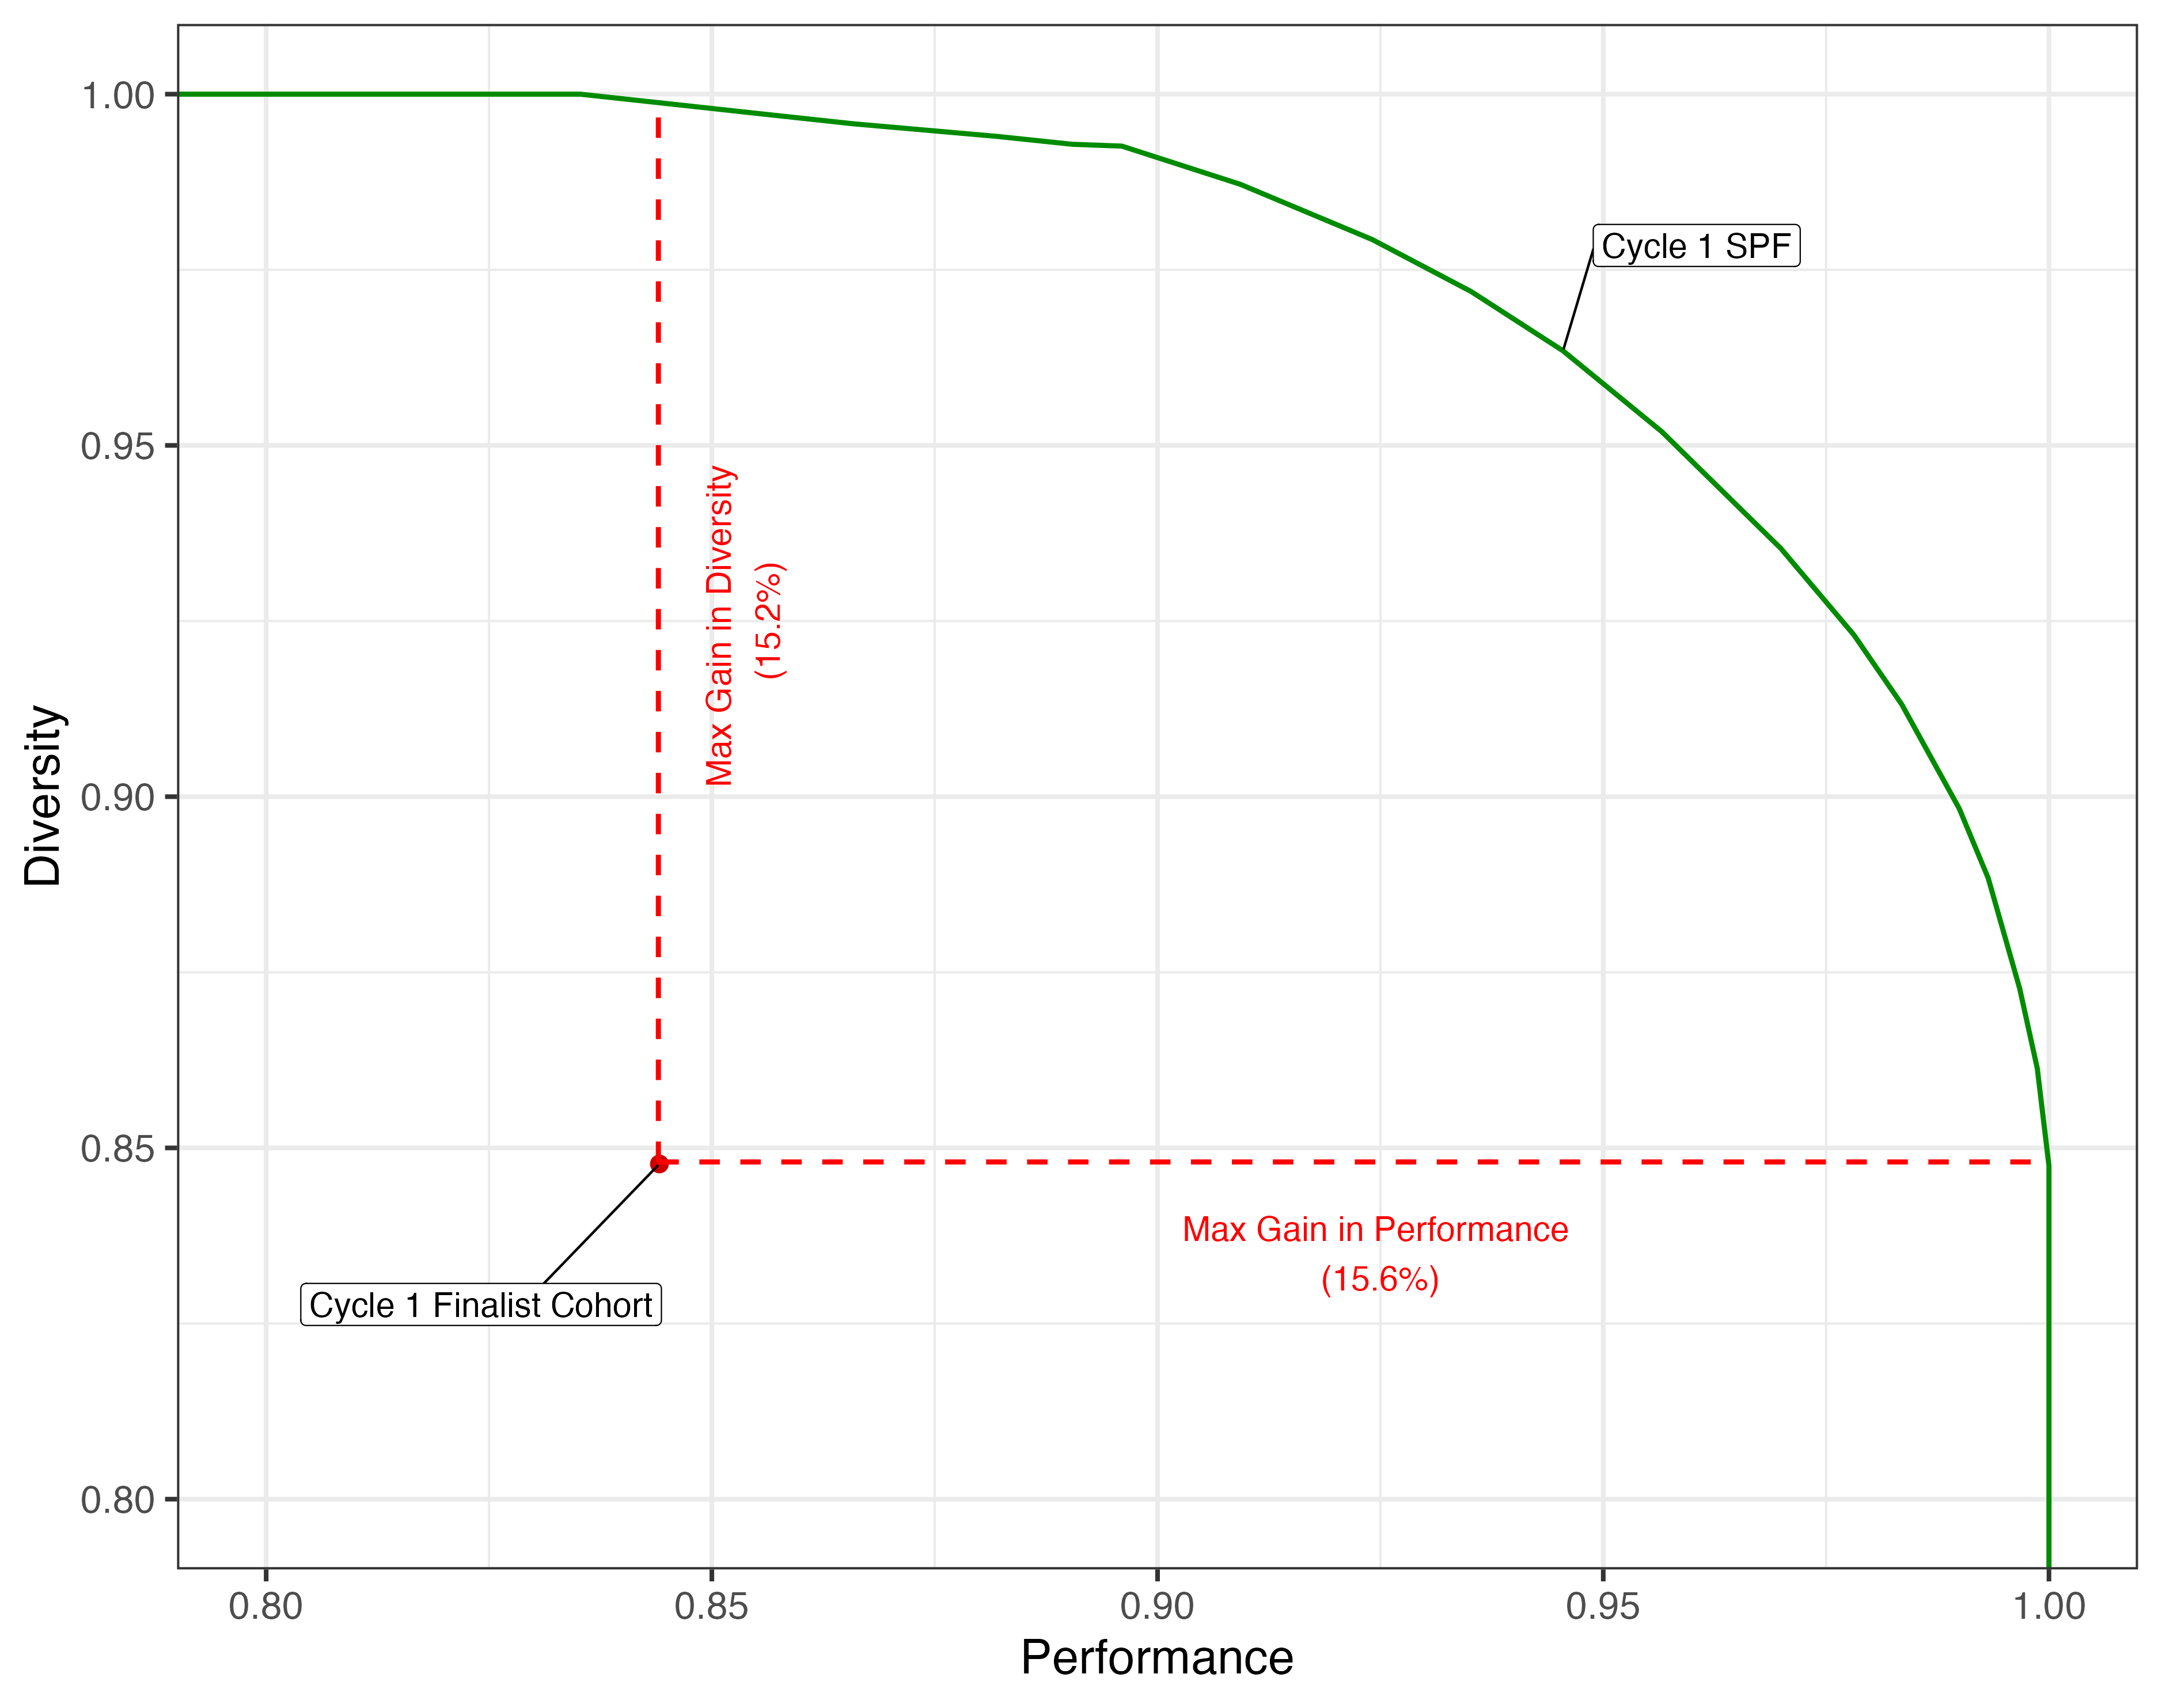
\includegraphics[width=\textwidth]{spf/yr1_spf_finalist.png}
        \caption{The SPF for the 2021 finalist selection process. In Cycle 2021, cohort diversity could have been improved by $15.2\%$ without any reduction in cohort performance, and cohort performance could have been improved by $15.6\%$ without any cost to diversity.}
        \label{fig:spf_2021}
    \end{subfigure}
    \hfill
    \begin{subfigure}[b]{0.4\textwidth}
        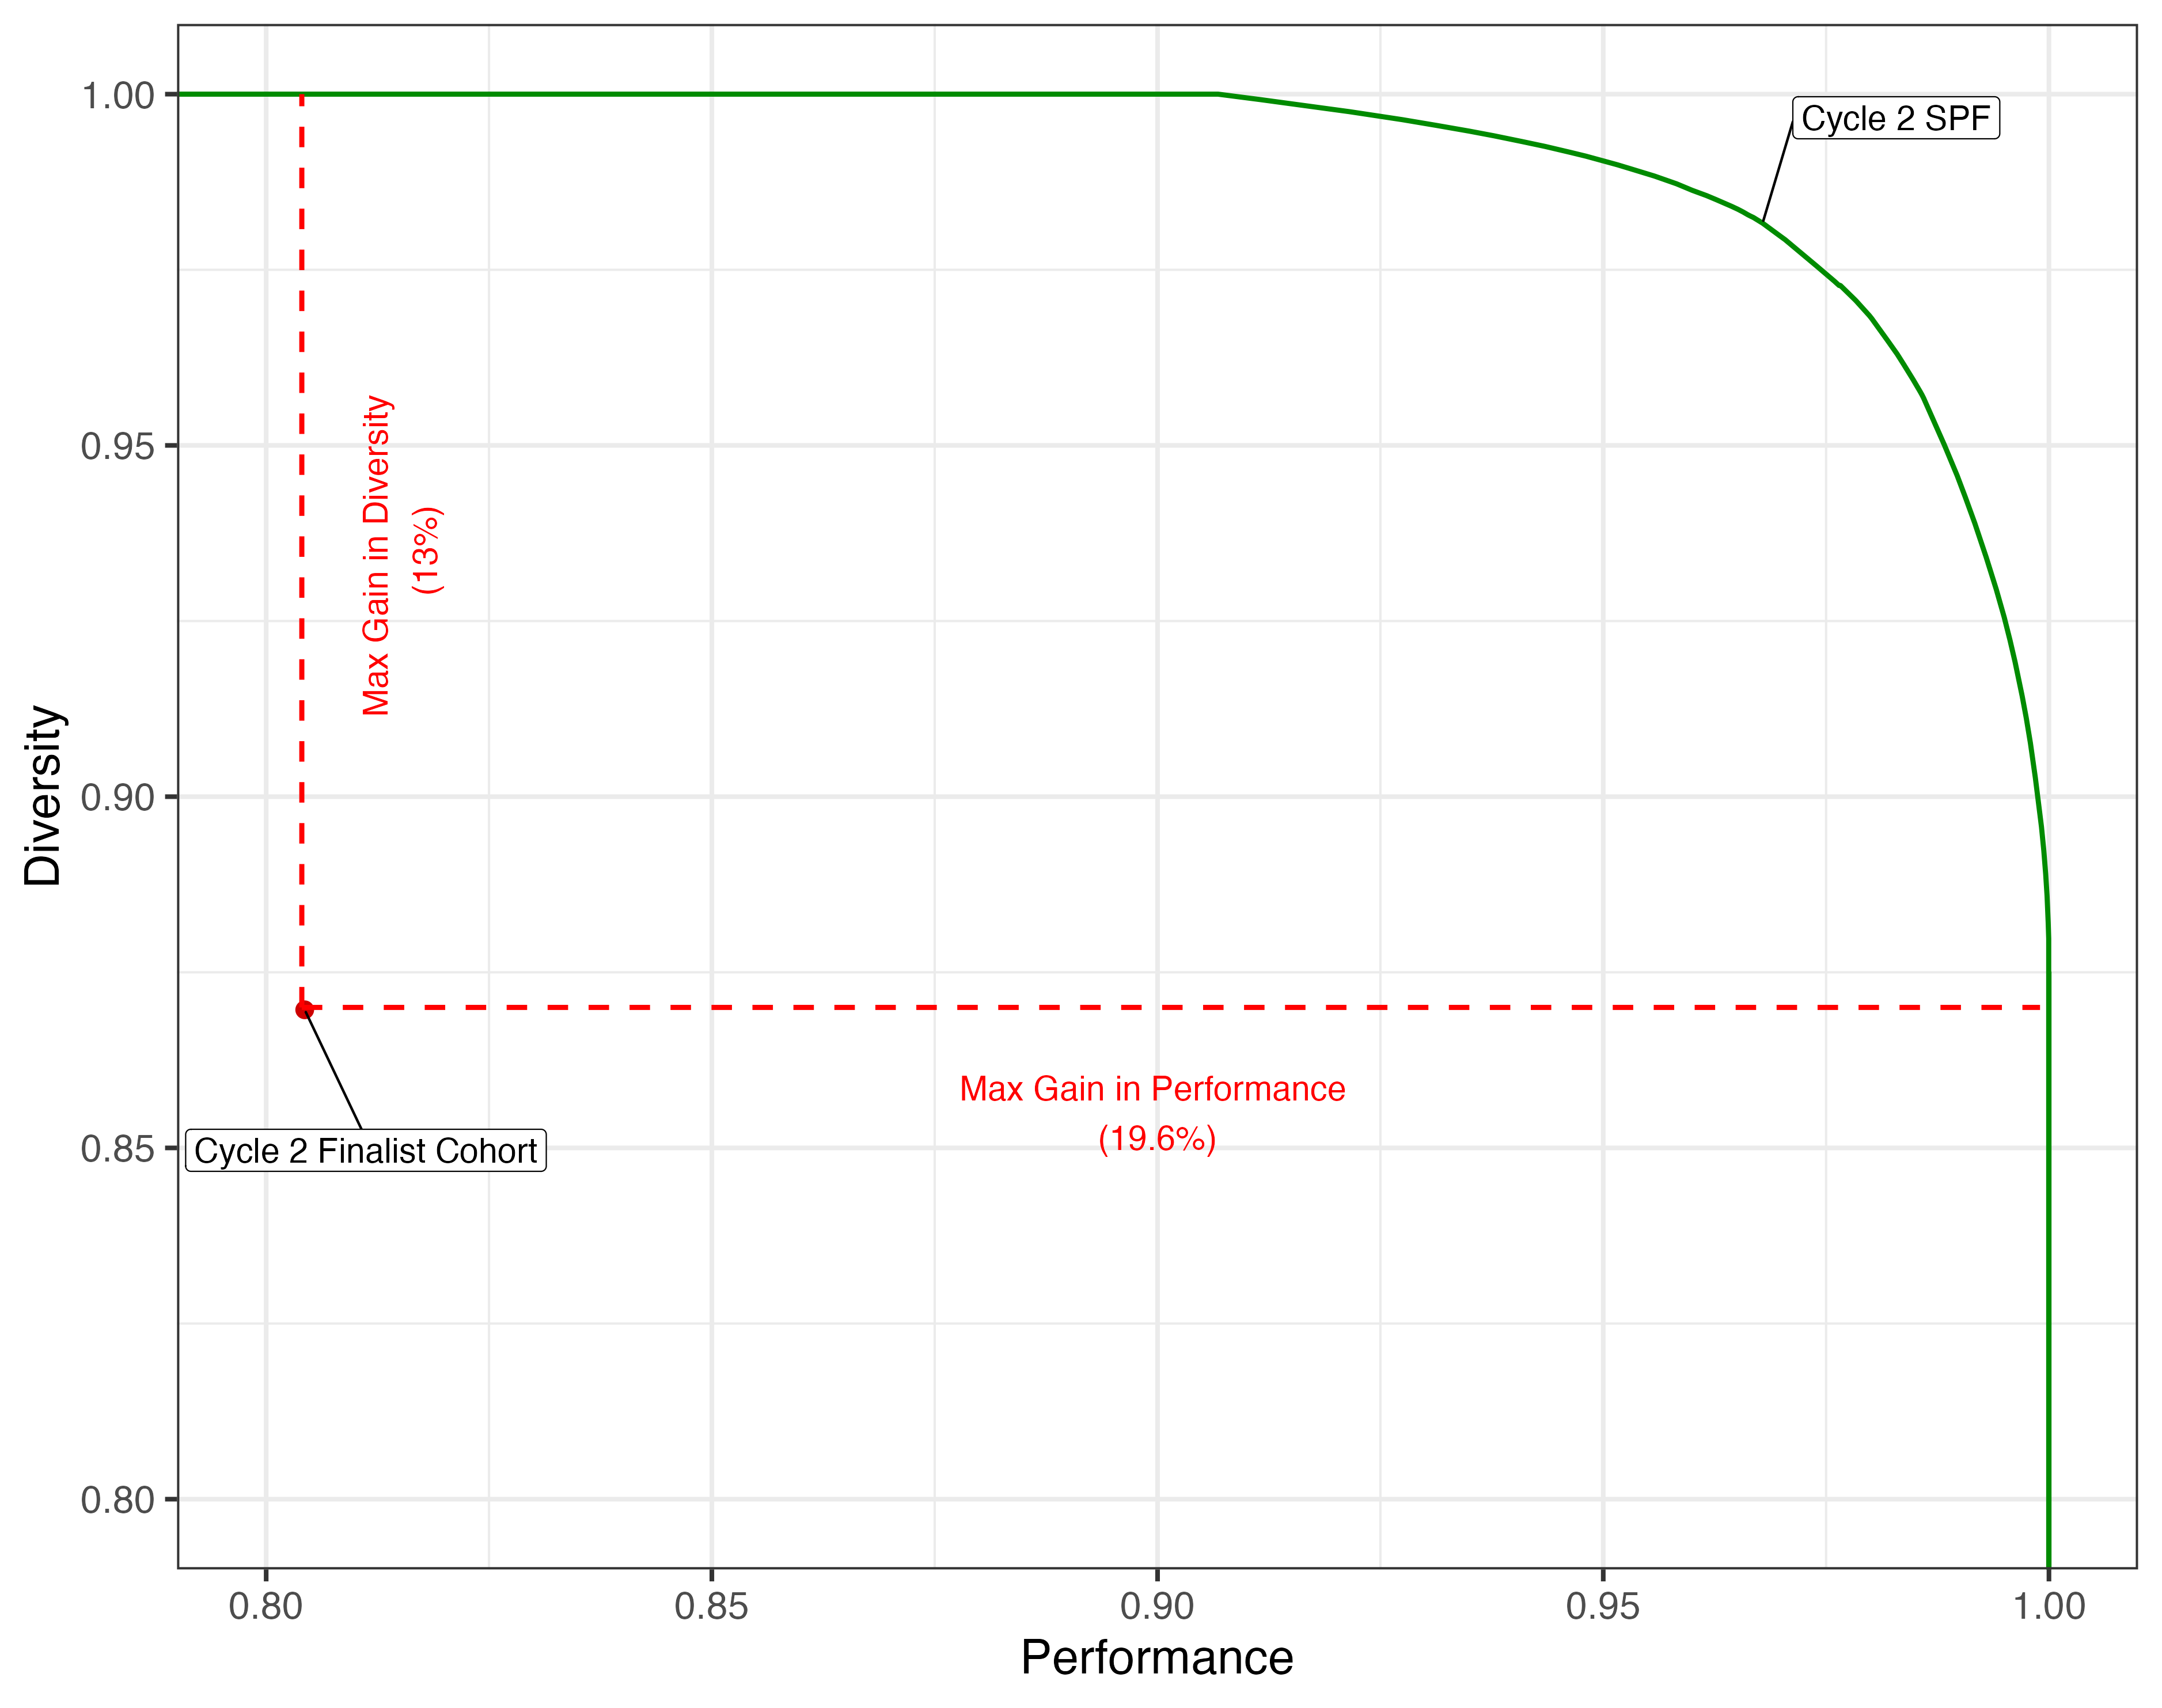
\includegraphics[width=\textwidth]{spf/yr2_spf_finalist.png}
        \caption{The SPF for the 2022 finalist selection process. In Cycle 2022, cohort diversity could have been improved by $13\%$ without any reduction in cohort performance, and cohort performance could have been improved by $19.6\%$ without any cost to diversity.}
        \label{fig:spf_2022}
    \end{subfigure}
    \caption{These figures depict the SPFs we estimate for the 2021 and 2022 finalist selection processes. The y-axis represents the diversity score while the x-axis represents average cohort performance (i.e. project scores). The green curve is our estimate of the cycle SPF, which represents the upper bound of diversity that is achievable at every level of cohort performance. The red dot depicts the actual level of diversity and performance of the finalists that were selected. The vertical and horizontal dashed red lines represent the maximum Pareto gain that was possible along the diversity and performance dimensions respectively. These figures are reproduced at a larger scale in Appendix \ref{app:spffigures}.}
    \label{fig:spf_2021_2022}
\end{figure}

The results from these two steps are depicted in Figure \ref{fig:spf_2021_2022}. Surprisingly, neither the 2021 nor 2022 finalist cohorts are chosen on the frontier. (We confirm that these apparent gap between frontiers and chosen cohorts are statistically significant using a permutation test in Figure \ref{fig:permutation_tests}.)

These results confound the simple model from Section \ref{ssec:measurement}, which suggests that organisations should always select cohorts on the frontier, as all cohorts within the frontier are dominated by cohorts that are either least as diverse and more talented or at least as talented and more diverse.

\paragraph{Evaluating Selection Decisions with Decision Support}
Now we turn to analyzing what happened to selection in the talent investment program when they were given access to our DST in Cycle 2023. Again, we first estimate the SPF. However, rather than immediately comparing chosen finalists to this estimate, we instead construct a functional implementation of Prototype \ref{fig:diversity} using this estimate (see Figure \ref{fig:spf_dst}).

\begin{figure}[htbp]
    \centering
    \caption{This figure displays the SPF-based DST provided to Rise selectors in Cycle 2023. In addition to the SPF itself, selectors were given access to a myriad of supporting information. While this information cannot all be presented here, much of it describes the candidate optima (i.e., the cohorts represented by the coloured dots). In particular, selectors were interested in the spread of performance scores in each cohort, as well as the extent to which each cohort satisfied program diversity targets.}
    \label{fig:spf_dst}
    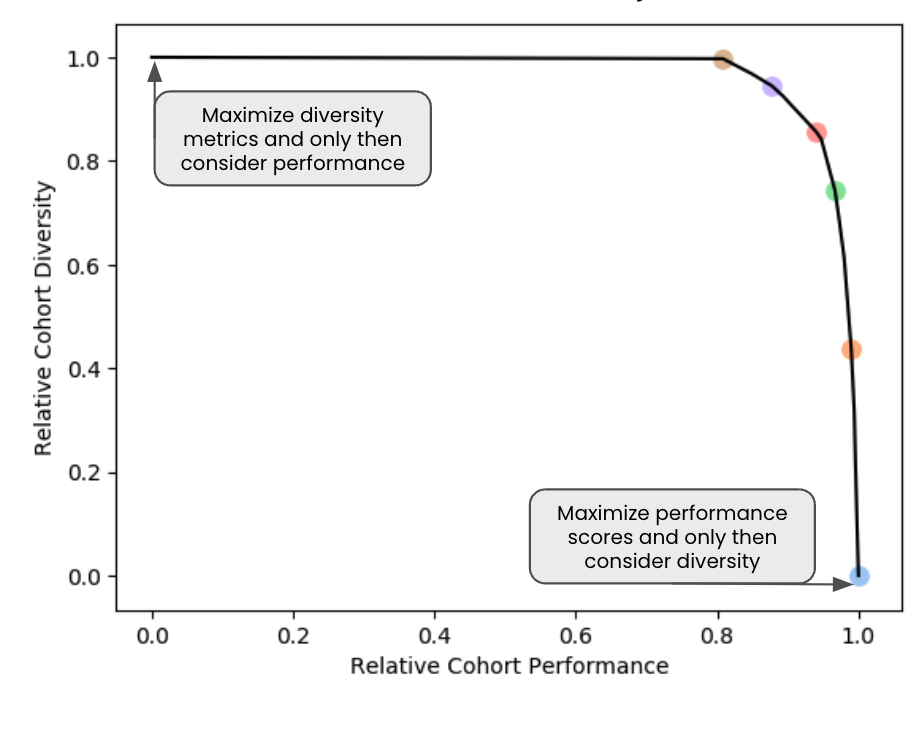
\includegraphics[width=.9\textwidth]{spf/spf_dst.png} 
\end{figure}

and then compare the finalist cohort's diversity and talent to the SPF estimate. The results from this analysis is depicted in Figure \ref{fig:spf_2023}. Here we see notable differences in the selection patterns relative to cycles 1 and 2. In particular, the cycle 3 finalist cohort is nearly on the SPF, making the possible Pareto improvements in both directions no more than $2\%$. This suggests two things. First, it provides further evidence that selection decisions in Cycle 2021 and Cycle 2022 were, in fact, inefficient; had Rise known about the possibility of making Pareto improvements with respect to their stated preferences, they likely would have changed their behaviour. Second, it provides evidence that the DST presented here actually influences the decisions of selectors. 

\begin{figure}[!htb]
    \centering
    \caption{This figure displays the SPF for the Cycle 2023 finalist cohort. Again, the y-axis represents the diversity score while the x-axis represents average cohort performance, the green curve is our estimate of the SPF, and the red dots depict the actual level of diversity and performance of the finalists that were selected. In this case, we overlay the finalist cohorts from 2021 and 2022 to provide a point of comparison. The diagonal dashed red line represents the distance in diversity-performance space between the Cycle 2022 cohort and the Cycle 2023 cohort. In Cycle 2023, there are no significant Pareto improvements on either diversity or performance.} 
    \label{fig:spf_2023}
    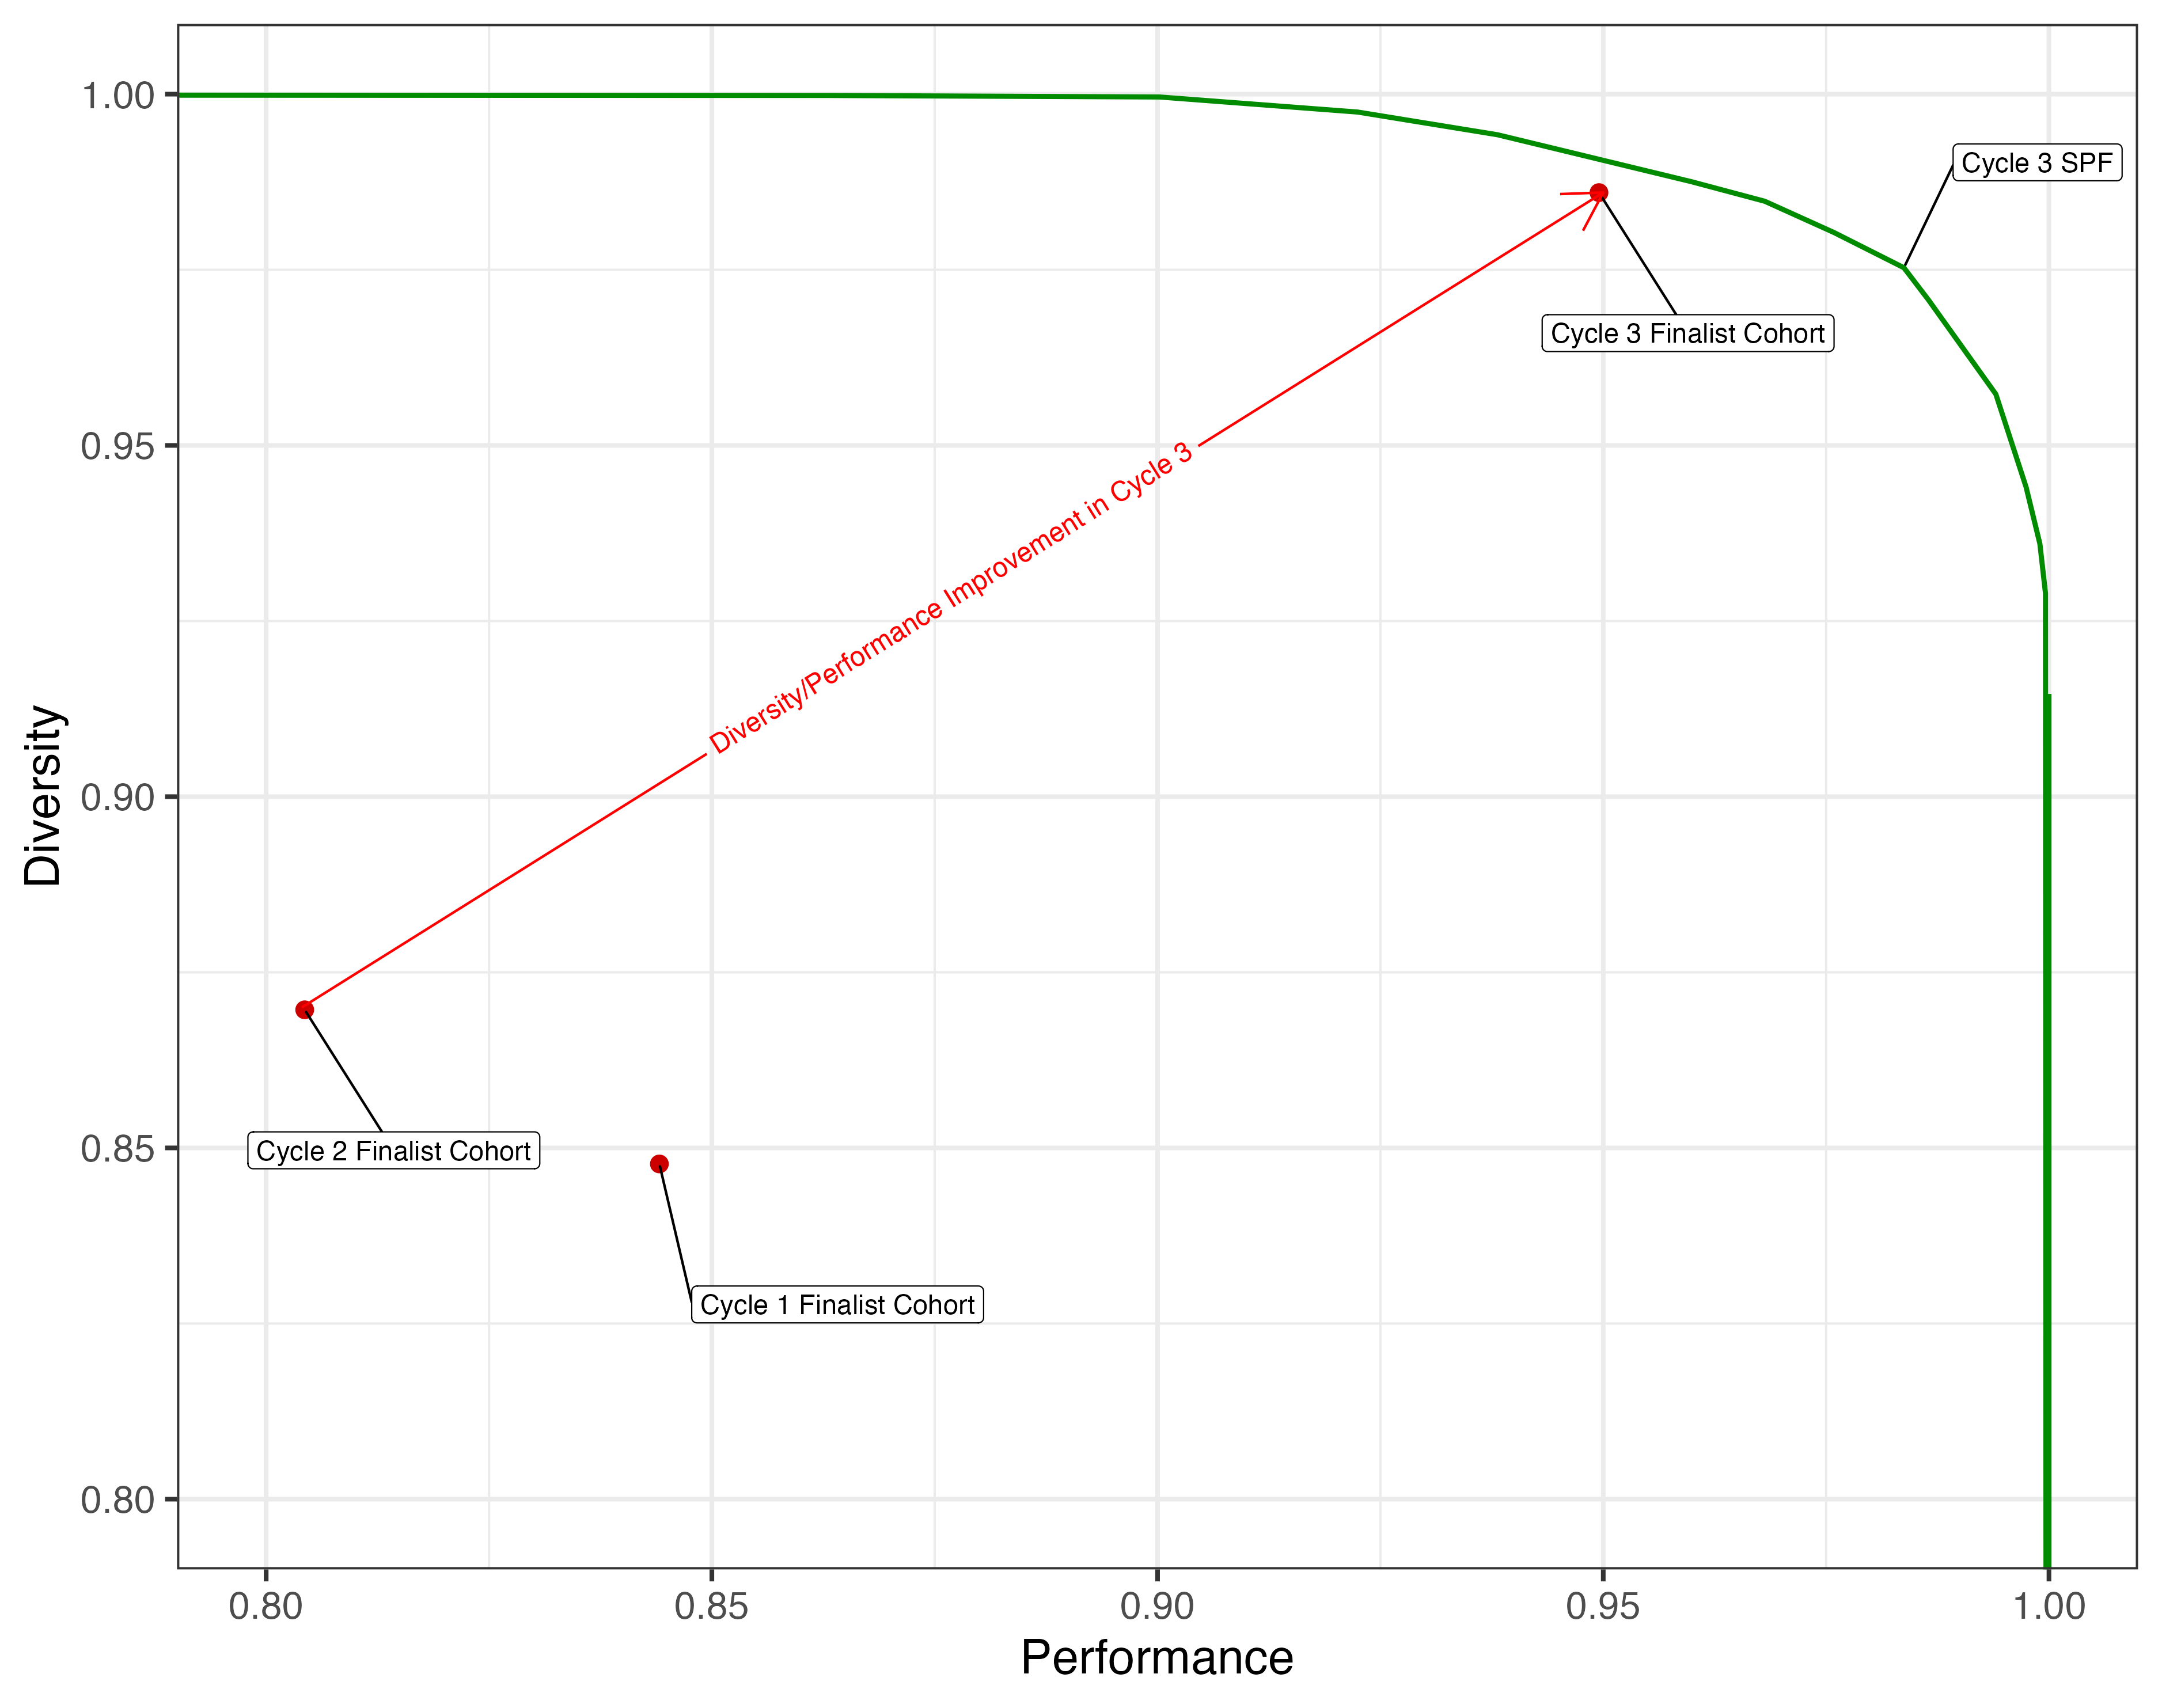
\includegraphics[width=.9\textwidth]{spf/yr3_spf_finalist.png}
\end{figure}

To determine whether the improvements are statistically significant, we leverage a permutation test depicted in Figure \ref{fig:permutation_tests}. The key comparison is between Cycle 2023 max Pareto improvements in talent and diversity (the solid blue vertical lines in both panels) and the corresponding 95 percentile of the random difference distributions (the dashed black vertical line). For both dimensions, the possible improvements are statistically insignificant. In contrast, Cycle 2021 and Cycle 2022 both display statistically significant max Pareto improvements. Ultimately, though this confounds the predictions about selector behaviour implied by the model in Section \ref{ssec:measurement}, it does suggest that the DST is effective in improving selection decisions.

\begin{figure}[htbp]
    \centering
    \caption{This figure displays permutations tests comparing the potential Pareto improvements along the diversity and talent dimensions to the distribution of differences on both dimensions from 1000 randomly drawn pairs of cohorts. The dashed black vertical line represents the 95 percentile of these differences. The solid vertical lines represent the max pareto gain on performance and diversity in each application year. We interpret inefficiencies at or larger than the 95 percentile of the distribution as significant, thereby sticking to the conventional $\alpha$ value. While Cycles 2021 and 2022 both appear to have significant inefficiencies, Cycle 2023 does not.}
    \label{fig:permutation_tests}
    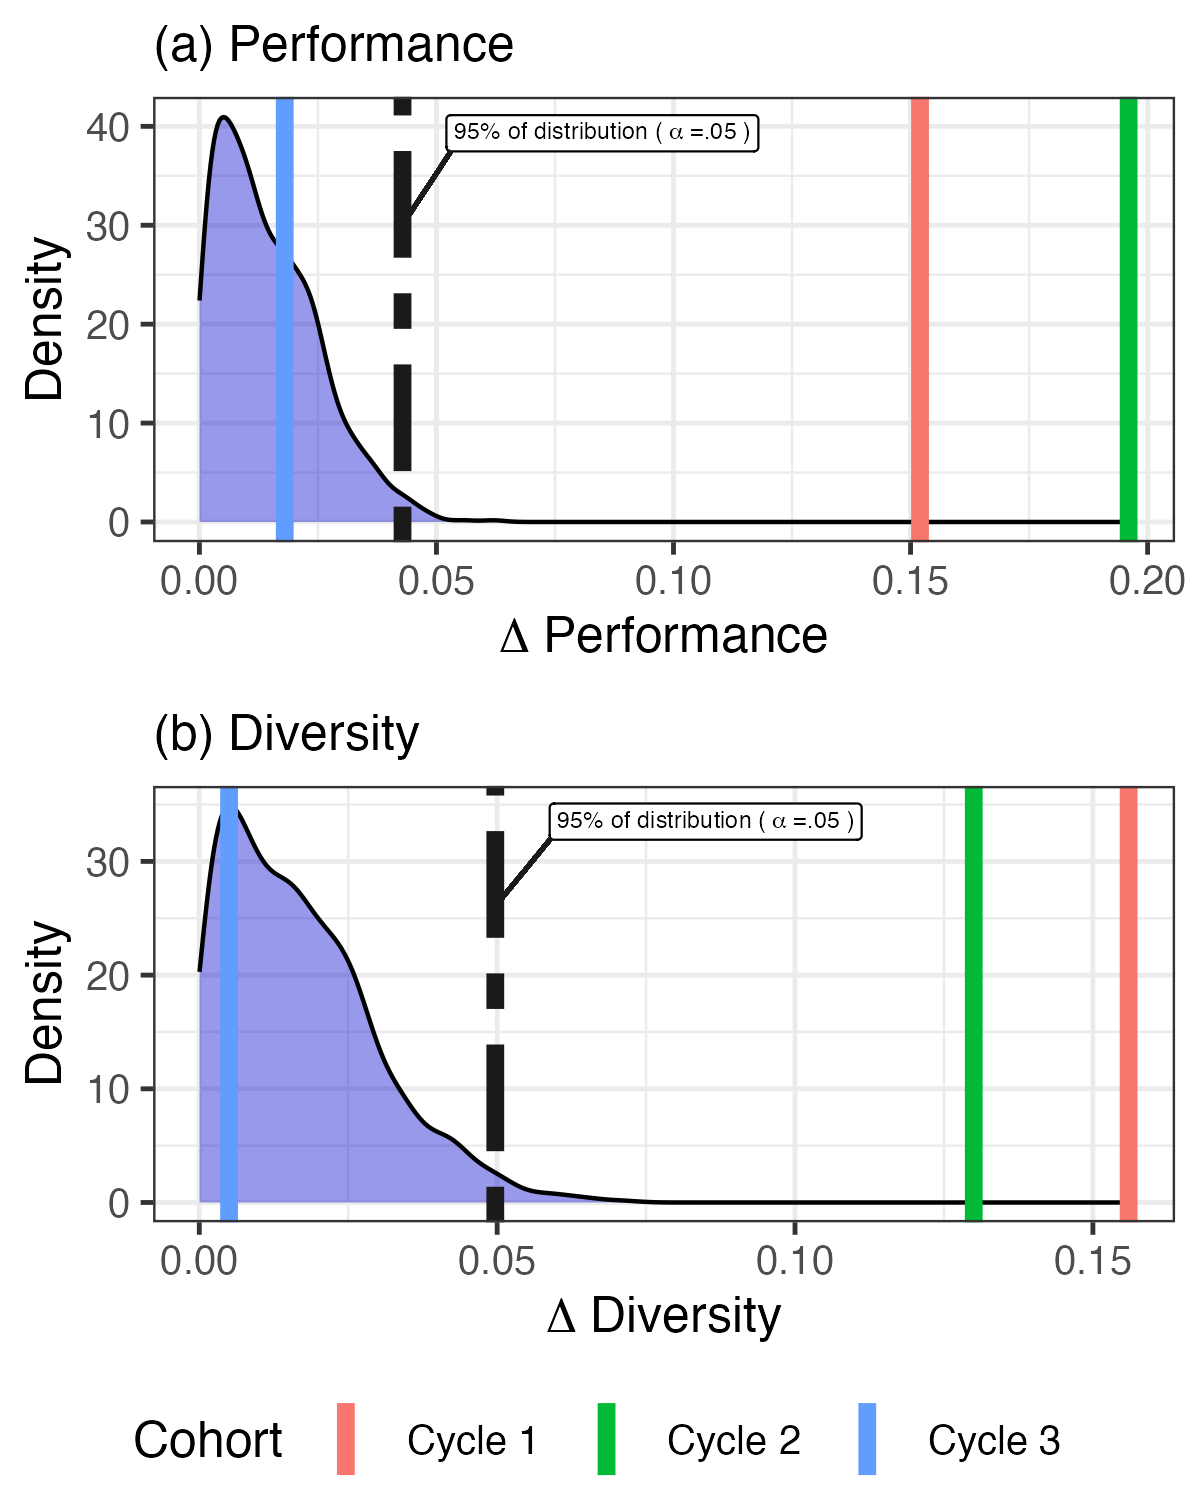
\includegraphics[width=.9\textwidth]{spf/permutation_tests.png} 
\end{figure}

\section{A Plausible Explanation for Selection Inefficiencies}\label{sec:spfexplanation}
\subsection{Why Are Organisations Selecting Pareto Inferior Cohorts?}\label{subsec:dts_nphard}
The results of our field study, specifically w.r.t. the 2021 and 2022 application cycles, suggest that organisations are not selecting cohorts on the SPF. This is surprising, as the SPF model suggests that organisations should always select cohorts on the frontier, as all cohorts within the frontier are dominated by cohorts that are either least as diverse and more talented or at least as talented and more diverse. In conversation with Rise, we have come to two plausible explanations for why this might be.

First, it might be that the axes of performance and diversity fail to capture the full dimensionality of organisational preferences. One mechanism for this, supported by the revelation from Chapter \ref{ch:diversity} that programs desire representations of specific idiosyncrasies, is that our axes fail to capture an idiosyncratic preference possessed by Rise selectors. Another mechanism, also supported by Chapter \ref{ch:diversity}, may come into play if the organisation's quantifications of talent do not capture the full scope of their concerns; i.e., if part of the measured ``talent'' an organisation selects for is only captured qualitatively, it cannot be factored into our model.

Second, however, it may be that there is an inherent cost associated with approaching the frontier. This would make organisational selections in the 2021 and 2022 application cycles second-best, in that they are optimal according to a model placing certain costs on their selections. 

The selection decisions in Cycle 2023 favour our second explanation; were there uncaptured preferences, we would expect these to play a similar role in Cycle 2023, and to result in an apparently suboptimal cohort selection. However, the cohort selected is, according to our model, Pareto optimal. Thus, we must seek out the cause of this inherent cost.

\subsubsection{Diversity Causes Complexity}\label{subsubsec:nphard}
The most plausible source of cost in approaching the frontier is the impracticality of selection teams discovering the frontier by hand. This is particularly sensible, as we prove here that calculating the frontier outright is $\mathbf{NP}$-hard; that is, there are no known efficient algorithms calculating the SPF outright \cite{COPPERSMITH198527}.

To see why, consider a college that aims to accept some target fraction of Black applicants from a pool of Black and white applicants. And, assume the school wants to select as talented a class as possible, where talent is proxied for by test scores, grades, or some combination of the two. In this special case, as shown in \textcite{kleinberg2018algorithmic}, there exists a computationally easy algorithm to calculate the SPF shown below.\footnote{Technically, the algorithm presented by \textcite{kleinberg2018algorithmic} only optimises for the \emph{most diverse} point on the SPF. Thus, we have added the \textbf{Repeat} step (cycling through the algorithm with different representation thresholds) to enable their algorithm to trace out the SPF.}

\begin{algorithm}
    \caption{A Procedure For Calculating the SPF Based on \textcite{kleinberg2018algorithmic}}\label{alg:kleinberg}
    \begin{algorithmic}
        \State \textbf{Define} a minority group (Black) and mutually exclusive majority group (white), 
        \State \textbf{Rank} applicants within their group by test score,
        \State \textbf{Define} a target proportion of Black admits,
        \State \textbf{Select} Black applicants from the highest ranking down until the target is reached,
        \State \textbf{Select} the white applicants from the highest ranking down for remaining slots,
        \State \textbf{Repeat} steps 1-5 for different thresholds of representation to trace out the SPF.
    \end{algorithmic}
\end{algorithm}

What allows this algorithm work is the \emph{mutual exclusivity} of the minority and majority group. This allows one to transform the diverse talent selection problem into two separate talent maximization problems where the organisation simply selects the most talented members of each group. This can be extended to any case where target proportions are defined at the level of mutually exclusive group level, even when multiple different demographic dimensions are considered. To be concrete, if the school actually cares about race and gender and, thus, has target proportions for black male, black female, white male, and white female applicants, then the problem can be broken into four separate talent maximization problems where the most talented members of each group are selected until the target proportions are met for each group. 

But what happens if an organisation has preferences for representation of \emph{non-mutually exclusive groups}? (I.e., what if an organisation places nonzero weight on two proportional diversity functions?) To continue the running example, this would be analogous to a college that has target proportions for black applicants and female applicants, but not for each race by gender combination. This seemingly small change prevents an organisation from transforming the problem into simpler group-specific talent maximization sub-problems. To see this, consider applying the \textcite{kleinberg2018algorithmic} algorithm to each group sequentially; this would mean selecting the best black applicants until reaching the target proportion, then doing the same for female applicants. If the most talented black applicants were male or if there are few talented white females in the pool, having allocated the black slots in this way forces the college to select less talented females than optimal (or, it may inhibit reaching the target proportion for females at all). In short, when diversity preferences are over non-mutually exclusive groups, we cannot cleanly break the problem into simple talent maximization subproblems for disjoint minority groups, so it is not clear how we might extend the \textcite{kleinberg2018algorithmic} algorithm to a general version of the diverse talent selection problem. 

The general diverse talent selection problem allows organisations to have preferences for representation of an arbitrary number of overlapping (or disjoint) demographic groups. This aligns more closely with the diversity preferences of real world organisations like colleges, firms, and social impact programs many of which aim to select personnel from various ethnicities, genders, classes, geographies, ideologies, and specialties. Organisations generally state their preferences using statements of the following form: ``the organisation desires at least $x\%$ of group $g$'' or ``the organisation desires at least one person from $m$ groups". These types of diversity preferences are what is formalised in the function $D(c)$, which forms an integral part of the class of functions $F$; we demonstrate here that calculating $F$ is $\mathbf{NP}$-hard.\footnote{We do this via `reduction' to the Vertex Cover. A reduction is simple: $A \leq B$ (i.e., $A$ reduces to $B$) if and only if there exists a polynomial time algorithm that makes some polynomially bounded number of calls to $B$ and thus returns an answer to $A$. In other words, we say that $A$ is $\mathbf{NP}$-hard if and only if $\forall B \in \mathbf{NP} A \leq B$. It is clear to see, then, that if $B$ is $\mathbf{NP}$-hard and $A \leq B$, then $A$ is also $\mathbf{NP}$-hard. For more details on reductions, see \textcite{10.5555/1074100.1074233}.}

We now prove that, for the class of functions $F$ of the form from Equation \ref{eq:f_spec}, the problem of finding the optimal subset of size $k$ for any $f_i \in F$ is still computationally complex. This time, we rely on the assumption that $\mathbf{NP}$-hard problems are computationally complex. That is, Theorem \ref{thm:specific-nphard} holds. 

\begin{theorem}\label{thm:specific-nphard}
    Let $U$ be a `universe' set of size at least $N \geq 2*n$ and $F = \{f: \mathcal{P} (U) \rightarrow \mathbb{R}\}$ be the set of functions described in Equation \ref{eq:f_spec}. Then $Opt_{spec}(f_i, n) := argmax_{c \in U \land |c| = n}(f_i(c))$ is $\mathbf{NP}$-hard in $n$.
\end{theorem}

In order to do this, and to justify the significance of this result, we bring in the computational complexity of the Vertex Cover problem, which has been proven to be $\mathbf{NP}$-hard \cite{COPPERSMITH198527}. Vertex Cover can be seen in Theorem \ref{thm:vertexcover}.

\begin{theorem}\label{thm:vertexcover}
    Let $G = (V, E)$ be a graph. Let $VC(G, \kappa) := Cov | Cov \subseteq V \land |Cov| = \kappa \land \forall e \in E . \exists v \in Cov . v \in e$ be a function of $G$ that returns a set $Cov$ such that every edge in $G$ is incident on at least one vertex in $Cov$. Then $VC$ in $\mathbf{NP}$-hard in the number of vertices.
\end{theorem}

We now prove Theorem \ref{thm:specific-nphard} by reduction to Theorem \ref{thm:vertexcover}, assuming that there exists no polynomial time solution to Vertex Cover \cite{COPPERSMITH198527}.

\begin{proof}
Suppose for a contradiction that Theorem \ref{thm:specific-nphard} admits some polynomial-time solution $Alg_{spec}$. I.e., $Alg_{spec}(s_i, k )= argmax_{c \in U \land |c| = n}(s_i(c))$.

\begin{algorithm}
    \caption{An Algorithm for $VC(G = (V,E), \kappa)$}\label{alg:vc_spec}
    \begin{algorithmic}
        \State \textbf{Consider} $U := E$
        \State \textbf{Define} $\vec{\mathbf{g}} := \{g_i = v_i \in e . e \in E | i \in |V|\}$ such that each $g_i$ has length $E$ and corresponds to whether an edge is incident on vertex $v_i$.
        \State \textbf{Return} $Opt_{spec}(1*D(c, \vec{\mathbf{1}}, \vec{\mathbf{0}}, \vec{\mathbf{0}}, \vec{\mathbf{g}}, \vec{\mathbf{0}})+ 0*P(c)) \geq k$
    \end{algorithmic}
\end{algorithm}

Then consider the algorithm $Alg_{VC}$ that is defined in Algorithm \ref{alg:vc_spec}. But this algorithm solves Vertex Cover in polynomial time relative to $Opt_{spec}$, and thus is a polynomial time solution to Vertex Cover. Assuming $\mathbf{P} \neq \mathbf{NP}$, contradiction!
\end{proof}

\subsection{Embedding Complexity into the Model}\label{subsec:dts_w_complexity}
Knowing the $\mathbf{NP}$-hardness of calculating the SPF outright, we can more comfortably assume that there exists a search cost in approaching the frontier; knowing that this $\mathbf{NP}$-hardness is driven by diversity targets, we can further suppose that this search cost is driven by diversity preferences. This leads us to a new model that incorporates complexity costs into the selection problem.

Consider a variation of the simple cohort selection problem (see Section \ref{subsec:simple_model}) where the organisation can search for increasingly diverse cohorts at a cost. Let the amount of search effort be $e\in[0,1]$ and define the cost of search effort be $\alpha p(e)$ where the cost is convex (i.e. $p_e>0$ and $p_{ee}>0$) and $\alpha$ is a constant that is inversely related to the quality of search technology available. Furthermore, we let the amount of search deterministically increase the maximum achievable diversity at each talent level, which is now given by $D^{SPF}*e$. The optimisation problem can then be rewritten as:

\begin{align}
&\max_{d,p,e} F\Big(d,p\Big) - \alpha p(e) \text{ \bf{ s.t. } } d = G(p)*e, \nonumber \\ 
& \implies \max_{p,e} F\Big(\underbrace{G(p)*e}_{\text{Info Cost}} ,p\Big) - \underbrace{\alpha p(e)}_{\text{Direct Cost}}. \label{eq:objective}
\end{align}

It is clear from the form of the organisation's new objective function in Equation \ref{eq:objective} that complexity of maximizing diversity imposes two kinds of costs: an information cost that represents the fact that the organisation will generally not know which cohort is on the SPF and a direct search cost. Also, when search costs are set to zero (i.e. $\alpha=0$), the problem collapses into the original problem because searching is costless and, therefore, maximized at $e=1$. But, when $\alpha>0$, the optimal cohort will now be inside of the SPF. This is because, for all $c'$ such that  $D(c')=G(p(c')=p')*e$ there exists $c^f$ on the SPF such that $D(c^f)=G(p(c^f)=p')$. Thus, as long as the optimal effort is below 1, any solution to this problem will result in selecting a cohort that is within the SPF and, therefore, non-first-best. The solution to the selection problem with complexity is depicted in Figure \ref{fig:model_complex}.

\begin{figure}[!htb]
    \centering
    \caption{This figure depicts an example solution to an iteration of the selection problem with complexity induced search costs, which is described in Equation \ref{eq:objective}. As in Figure \ref{fig:model_spf}, the solid blue curve represents the SPF, the dotted blue curve represents the organisation's indifference curve corresponding to the highest achievable utility without search costs, and the blue dot represents the diversity and performance of the first-best solution. Additionally, the solid red curve represents the accessible frontier with optimal search, the dotted red curve that represents the highest achievable utility with search costs, and the red dot that represents the diversity and performance of the optimal cohort with search costs (i.e. the second-best solution).}
    \label{fig:model_complex}
    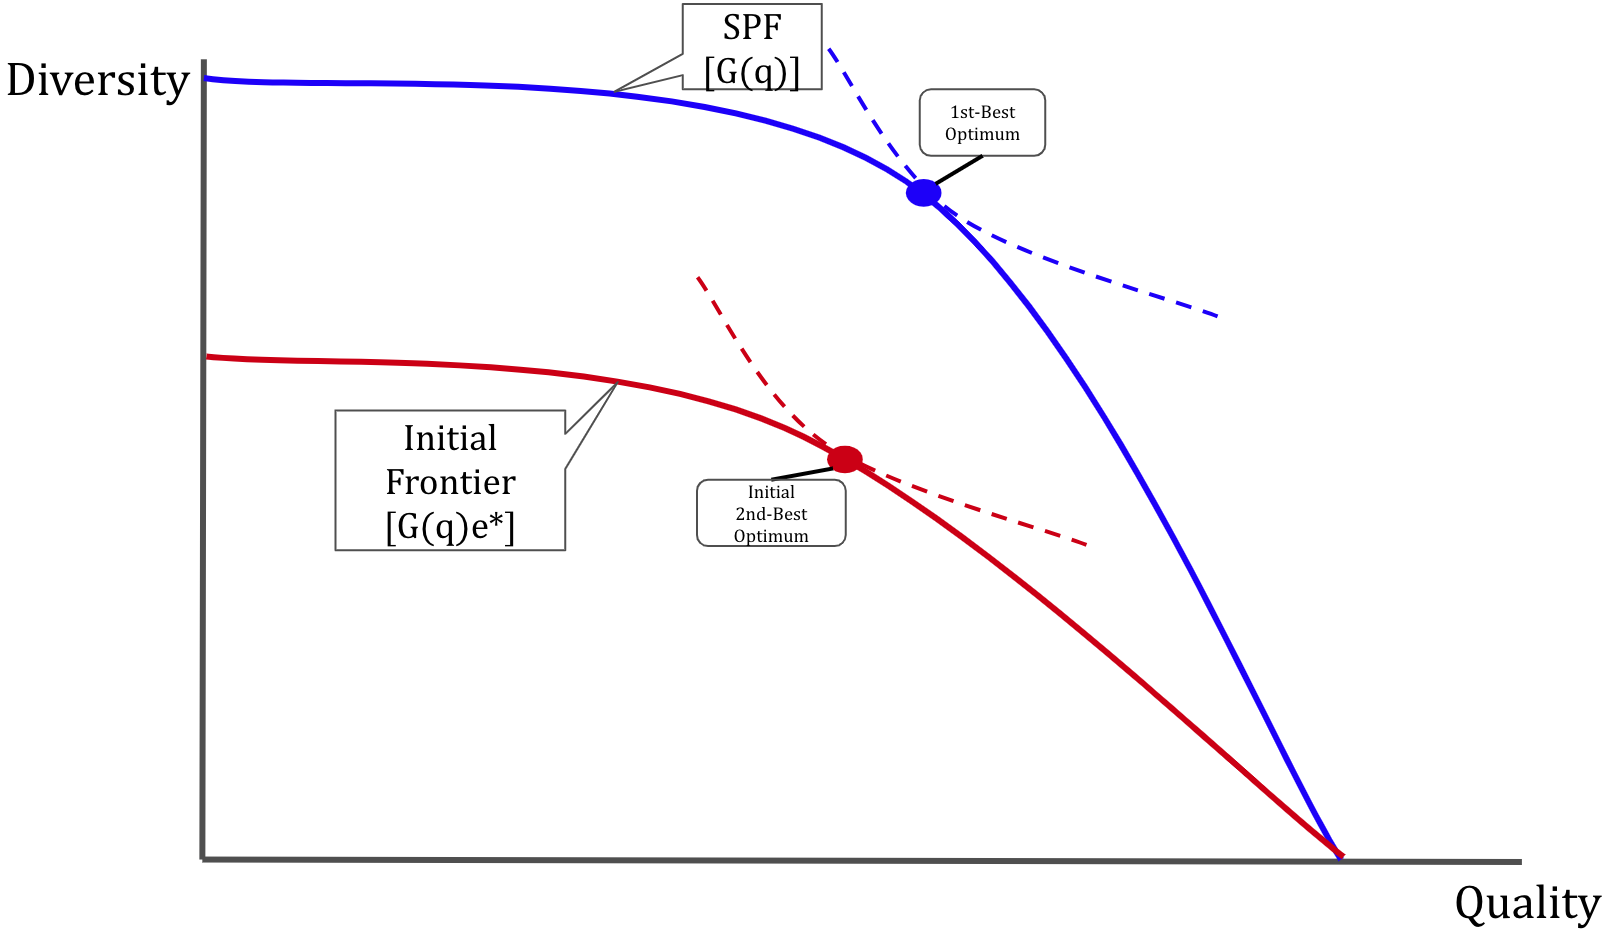
\includegraphics[width=1\textwidth,height=\textheight,keepaspectratio]{spf/model_complex.png} 
\end{figure}

Additionally, the extent of the inefficiency will tend to reduce as complexity costs reduce. We can see this by examining the comparative statics of the model. To simplify our derivation of the relevant comparative static, we refer to the organisation's objective function as $O(p,e)\equiv F\Big(G(p)*e ,p\Big) - \alpha p(e)$. Furthermore, we use subscripts on functions refer to partial derivatives and we drop the arguments of functions where this causes no confusion. The (necessary) first order conditions from this model are, therefore, the following:

\begin{align}
O_p & \equiv F_{d}(G(p)e,p)G_p(p)e + F_p(G(p)e,p) = 0 \nonumber \\
O_e & \equiv F_{d}(G(p)e,p)G(p) - \alpha p_e(e) = 0. \nonumber
\end{align}

To ensure this is a maximum, we also need to assume that the (sufficient) second order conditions hold. They are the following:

\begin{align}
O_{pp} \equiv &\;  e^2G_p^2F_{dd} + 2eG_pF_{dp} + eG_{pp}F_d + F_{pp} < 0, \nonumber \\
O_{ee}  \equiv &\;  G^2F_{dd} - \alpha p_{ee} < 0, \nonumber \\
&  \; O_{ee}O_{pp} - O_{ep}^2 > 0, \nonumber
\end{align}

\noindent where $O_{ep} \equiv O_{pe} \equiv eGG_pF_{dd} + F_dG_p + GF_{pd}$. Under these conditions, solutions to the first order conditions both exist and guarantee a maximum. These solutions can be defined as $p^*(\alpha)$ and$e^*(\alpha)$. If we plug this into the first order conditions and take a derivative with respect to $\alpha$, which governs the complexity costs, we get the following system of equations:

\begin{align}
& O_{pp}\frac{\partial p^*}{\partial \alpha} + O_{pe}\frac{\partial e^*}{\partial \alpha} + O_{p\alpha} \equiv 0, \nonumber \\
& O_{ep}\frac{\partial p^*}{\partial \alpha} + O_{ee}\frac{\partial e^*}{\partial \alpha} + O_{e\alpha} \equiv 0  \nonumber
\end{align}

\noindent where $O_{e\alpha} = -p_e$ and, essential for signing the comparative static, $O_{p\alpha} = 0$. We can then solve for $\frac{\partial e^*}{\partial \alpha}$ algebraically (or using Cramer's rule), which gives the following:

\begin{equation}
\frac{\partial e^*}{\partial \alpha} = \frac{-O_{e\alpha}O_{pp}}{O_{ee}O_{pp} - O_{ep}^2} + \cancelto{0}{\frac{O_{ep}O_{p\alpha}}{O_{ee}O_{pp} - O_{ep}^2}} = \frac{p_eO_{pp}}{O_{ee}O_{pp} - O_{ep}^2} < 0, \label{eq:comp_stat}
\end{equation}

\noindent where the the final inequality holds because of the signs assumed in the first and third second order conditions. Thus, as complexity costs rise, optimal search effort decreases.

This model, thus, implies two predictions about organisational behaviour: (1) when complexity-induced search costs are sufficiently high, organisations will select cohorts within the SPF and (2) as computational costs are reduced, organisations will select cohorts that are closer to the SPF. We have already seen in Section \ref{sec:spfresults} that both predictions hold in practice.

\section{Alternate Applications of the SPF}\label{sec:spfapplications}
The main body of this chapter implements and evaluates Prototype \ref{fig:diversity} as an \emph{in-process} DST by conducting Action Research with the Rise program. However, in this section, we discuss potential \emph{ex-post} applications of the SPF.

\paragraph{Comparing the Diversity Cost of Alternative Talent Measures} In some cases, organisations may have multiple alternative talent measures that seem equally valid as measures of individual ability. In this case, the tradeoff between each measure and diversity may help an organisation decide which talent measure they prefer.  Two cases where this might be relevant are in hiring and college admissions. In hiring, firms may have multiple measures that predict applicant productivity, but have many ways to weight the various measures that are roughly equivalent for productivity prediction \cite{hartigan_fairness_1989}. This can happen if productivity is multidimensional (e.g. work per hour, tenure, spillovers on others, etc.), and different measures are correlated with some dimensions and not others. As similar problem can be faced in college admissions, where, again, the college has multiple measures of applicant ability and may be close to indifferent about some set of ways of combining them when judging an applicant's talent \cite{tam2002new}. 

In these cases, the SPF estimation procedure allows an organisation to consider another dimension: which talent measures demand the sharpest tradeoffs against cohort diversity? I.e.: which measures yield the smallest SPFs? This is particularly relevant in cases where preferences may be lexicographic, meaning that an organisation wants to maximize on talent first, then, conditional on doing so, choose the cohort among top talent cohorts who is the most diverse possible. It also is relevant in contexts where an organisation is not allowed, either legally or internally, to explicitly prioritise diversity in its selection criterion, but still wishes to promote diversity \cite{Bleemer_2023}. 

We demonstrate how to use SPF estimation to compare the diversity tradeoffs of two alternative talent measures. To do this, we estimate the SPF twice, once using each of the talent measures, and then compare the level of diversity at each percentile of both measures. In the case of indifference between the two talent measures on the talent dimension, the measure with higher maximum achievable diversity in the relevant percentile range should be chosen if the organisation cares at all about diversity. We use two measures of talent collected by Rise: a project-based measure and a traditional score. The results of this comparison are depicted in Figure \ref{fig:compare_div_tradeoffs}. Given that the program does care about diversity, this would justify using project quality instead of the traditional score for selection. 

\begin{figure}[htbp]
    \centering
    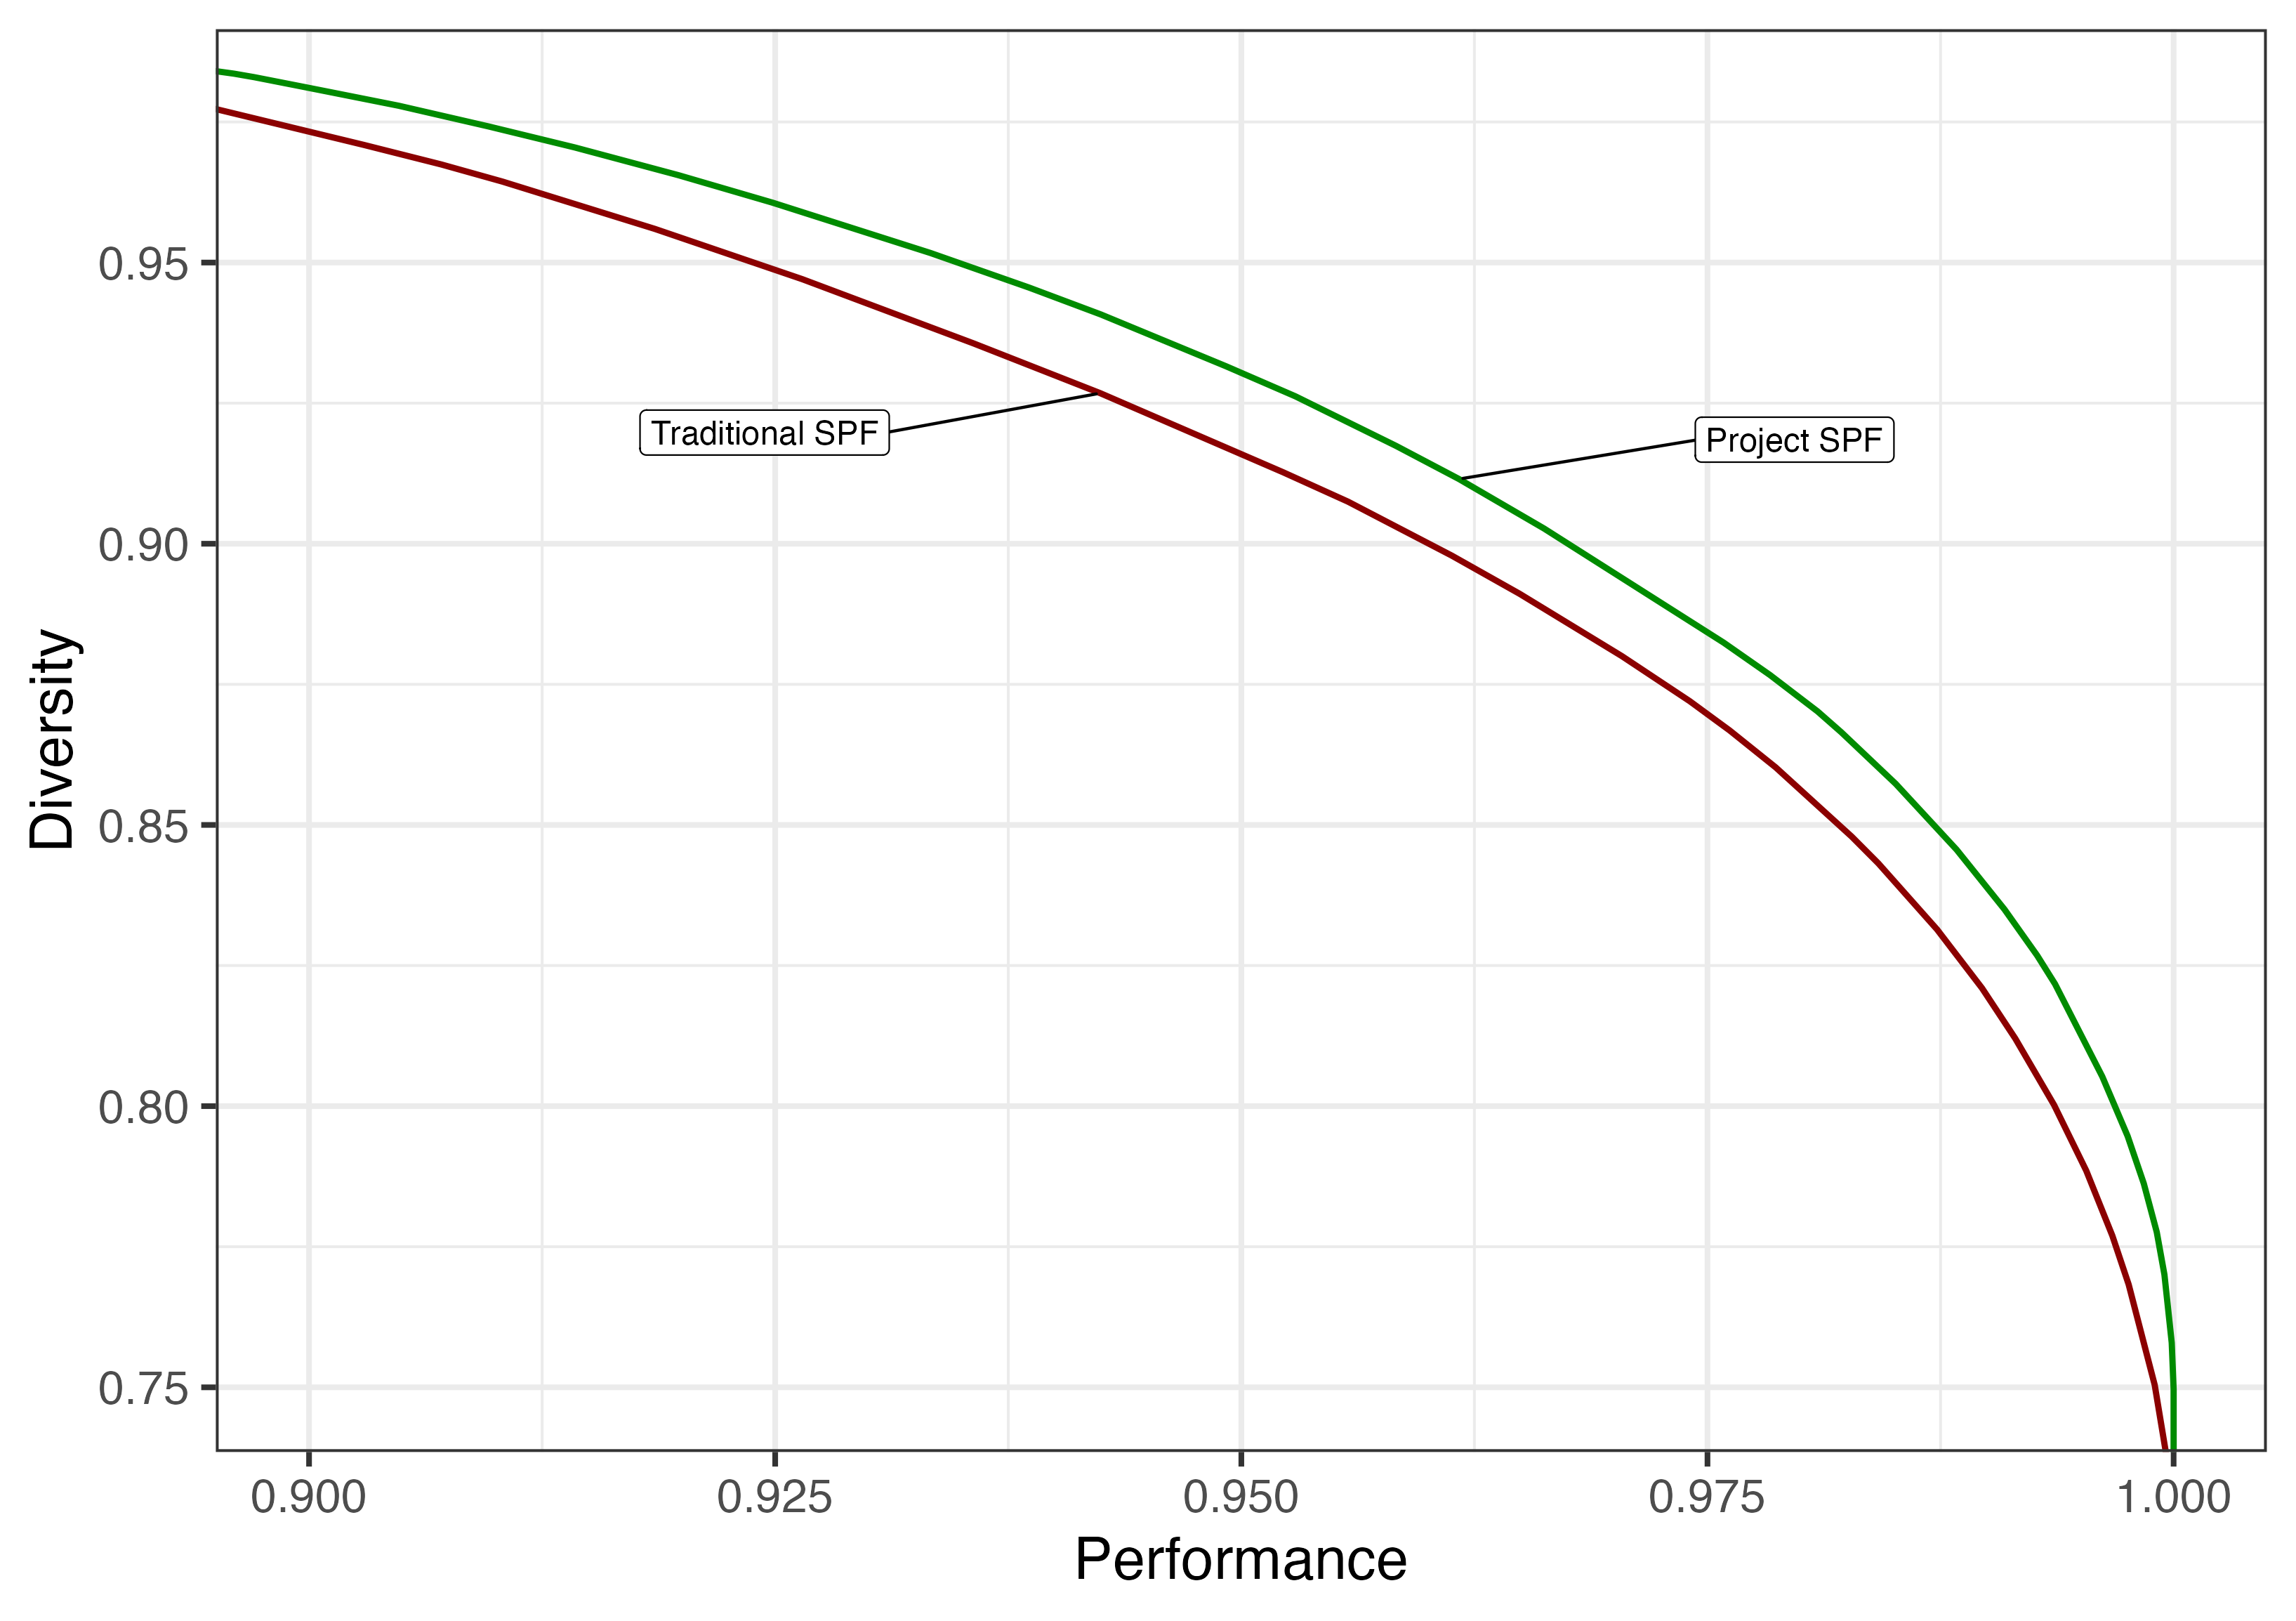
\includegraphics[width=\textwidth]{spf/alt_merit_spfs.png} 
    \caption{This figure displays the SPF we estimated for the cycle 1 finalist cohort and an SPF based on a more traditional method of measuring performance (i.e. the average of cognitive ability and an essay assessment). The y-axis represents the diversity score while the x-axis represents average cohort performance on projects or the traditional score. The vertical distance between the SPFs represents the difference in maximal diversity conditional on a cohort performing at a particular percentile of both scores. We see here that, above the 90th percentile of talent for both measures, the project quality measure strictly dominates the traditional score in diversity.}
    \label{fig:compare_div_tradeoffs}
\end{figure}
        
This method can also be applied to compare the diversity-talent tradeoff across application years. To do this, simply estimate SPFs for each application cycle and compare the level of diversity at each percentile of talent. As long as the diversity goals remain the same each year and cohort diversity is renormalized such that the most diverse cohort across all years becomes 1, organisations can compare across years to see whether differences in applicants across years better afford getting closer to their goals. Figure \ref{fig:diversity_across_cohorts} shows just this comparison. In general, the Cycle 2023 SPF allows for selecting more diverse cohorts at every level of talent than the other two cohorts. But, whether Cycles 2021 or 2022 allow for more diversity depends on where in the talent distribution the program is interested in. Near the top of the talent distribution, the Cycle 2022 has more diverse cohorts, but this flips as talent falls below the 94th percentile.

\begin{figure}[!htb]
    \centering
    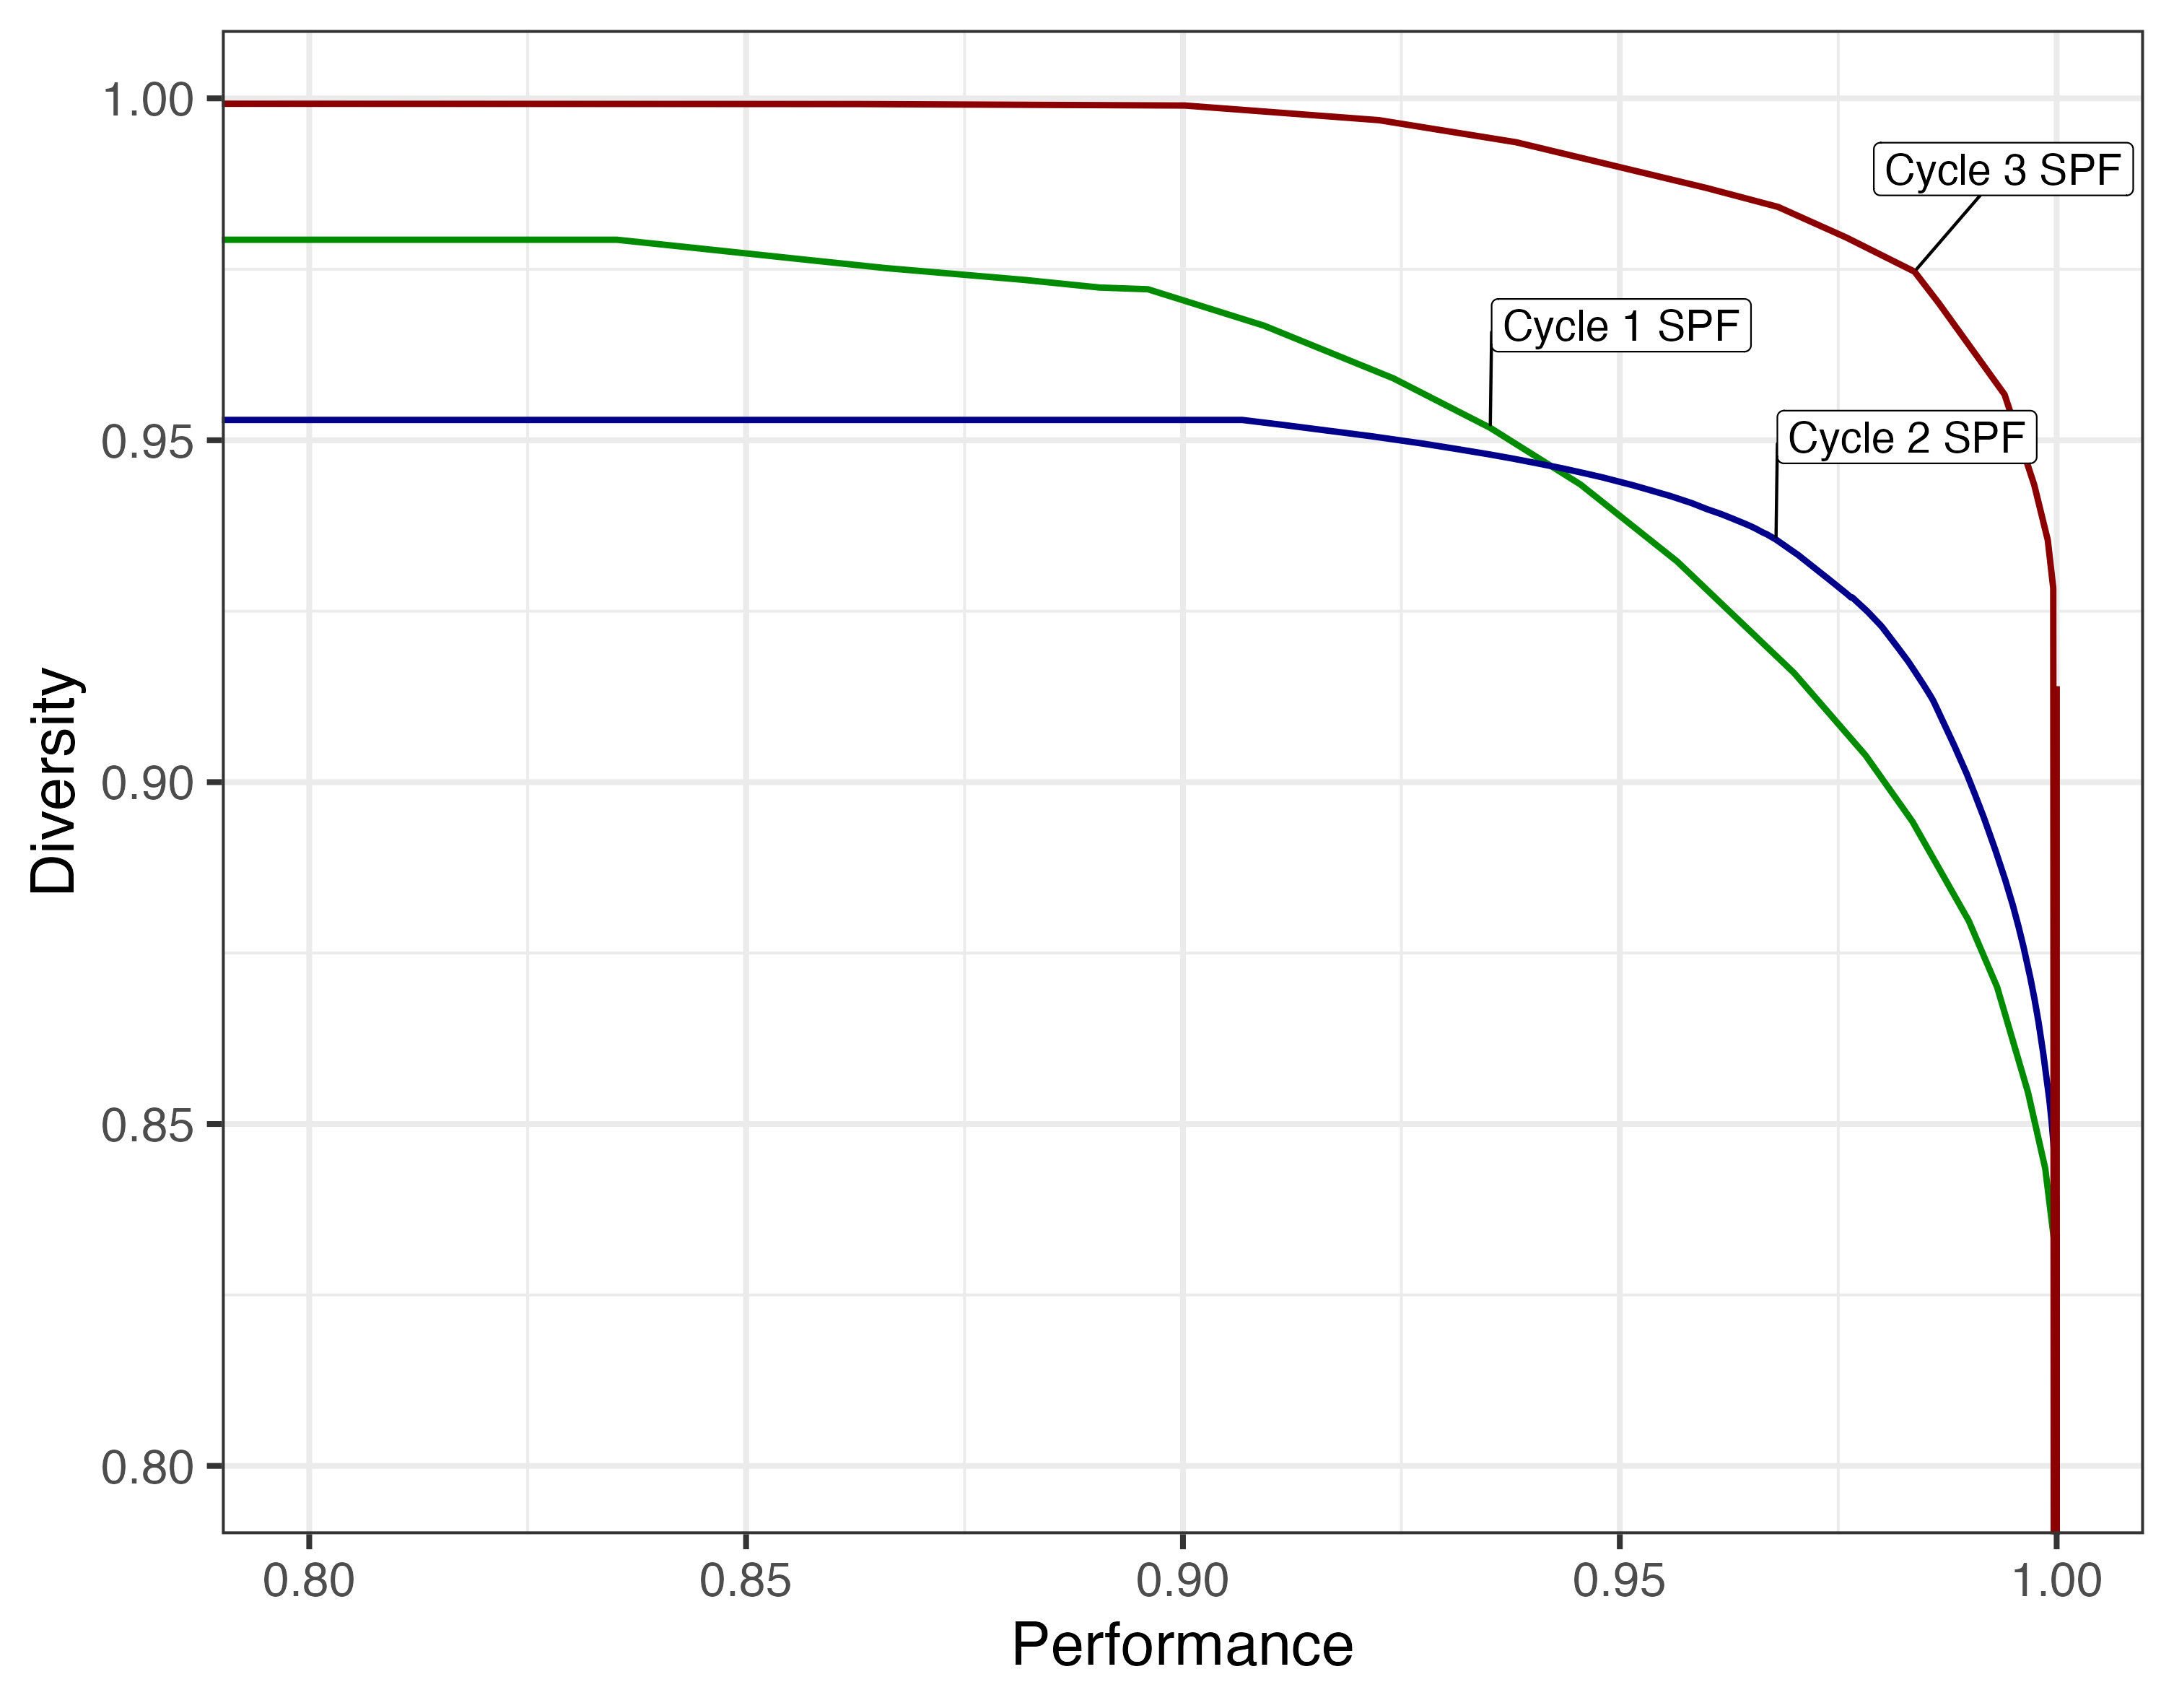
\includegraphics[width=\textwidth,height=\textheight,keepaspectratio]{spf/spf_cohort_comparisons.png} 
    \caption{ This figure displays the SPFs we estimate for three finalist cohorts. The y-axis represents the diversity score while the x-axis represents average cohort performance (i.e. percentiles of mean project scores). The diversity target is held constant across cohorts, so differences in SPFs conditional on performance represent differences in the capacity to reach the same diversity target at a given level of performance.}
    \label{fig:diversity_across_cohorts}
\end{figure}

\paragraph{Evaluating Alternative Selection and Screening Approaches} Relatedly, organisations may consider using cheaper, but lower quality measures of talent to screen or select applicants. For example, firms may consider using metrics (e.g. cognitive or personality assessments) or recruiters to screen their applicant rather than allow each applicant to be assessed via an interview. In some cases, organisations may be considering replacing costlier selection measures and selecting applicants entirely on the basis of cheaper information. Unlike before, we now assume that the initial metric captures talent much better than the new metric. Thus, rather than comparing different SPFs, we place cohorts selected using new metrics on the SPF estimate drawn using the original metric. If the new metric is not too much worse than the original metric, then the new metric may be a better choice.

Running selection counterfactuals can be done using two types of designs: the first we will refer to as a ``causal'' design and the second we call a ``suggestive'' design. A causal design requires an organisation to run a screening experiment where applicant talent is either evaluated randomly (or all applicants are evaluated). This allows organisations to avoid the selective labels problem whereby results become biased due to selection of who gets evaluated and who doesn't. Avoiding this problem allows organisations to analyze representative samples, meaning that comparisons between alternatively selected samples and the estimated SPF should extend to the full population of applicants. Thus, barring any significant contextual changes, that the results will be the same (in expectation) when used on another applicant pool (in this sense, the results are ``causal''). Alternatively, a counterfactual exercise can be conducted on selected data where only a selected set of individual's talent is assessed. In this case, the applicability of the results to another applicant pool is merely ``suggestive'', hence the name ``suggestive design''. Causal designs, though more useful for decision-making, are also more costly, as they require running a selection experiment, which may force organisations to miss out on talent (additionally, using known-inferior selection methods may pose a fairness concern). 

To demonstrate, we return to the talent investment program example where, in Cycle 2021, we can assess alternative selection procedures using a causal design. This is because, in Cycle 2021, the program ran a selection experiment to determine whose projects were reviewed. In particular, the program used a weighted sum of applicants' cognitive ability and peer assessments of their video essays to select the top $1500$ applicants who would receive project reviews. Of the remaining applicants, $500$ were chosen at random to be evaluated as well. This means that, from the total application pool of $2800$, a representative sample can be reconstructed by re-weighting the $500$ randomly assessed applicants such that they represent all $1300$ applicants who were below the project review threshold.

To demonstrate the use of the SPF estimate for counterfactual selection analysis, we compare the efficacy of three alternative selection strategies: the cognitive score, the traditional score, and the peer score. Because the cognitive score and the traditional score both use measures that are closely related to typical talent measures, this comparison also serves as a substantive comparison of traditional selection methodologies and more experimental ones, such as using applicant peer review. The results of this comparison are depicted in Figure \ref{fig:alt_screen}. Here we see that, on the dimension of talent (as measured by project quality) the cognitive ability score performs the worst of the three by far (over $10\%$ worse than the other two scores). The traditional score performs slightly better than the peer score on talent, but the peer score (and the cognitive ability score) performs slightly better than the traditional score on diversity. What is perhaps most striking, however, is that all three alternative selection approaches result in cohorts well within the frontier, indicating that Rise's actual metric far outstrips each hypothetical alternative.

    \begin{figure}[!htb]
    \centering
    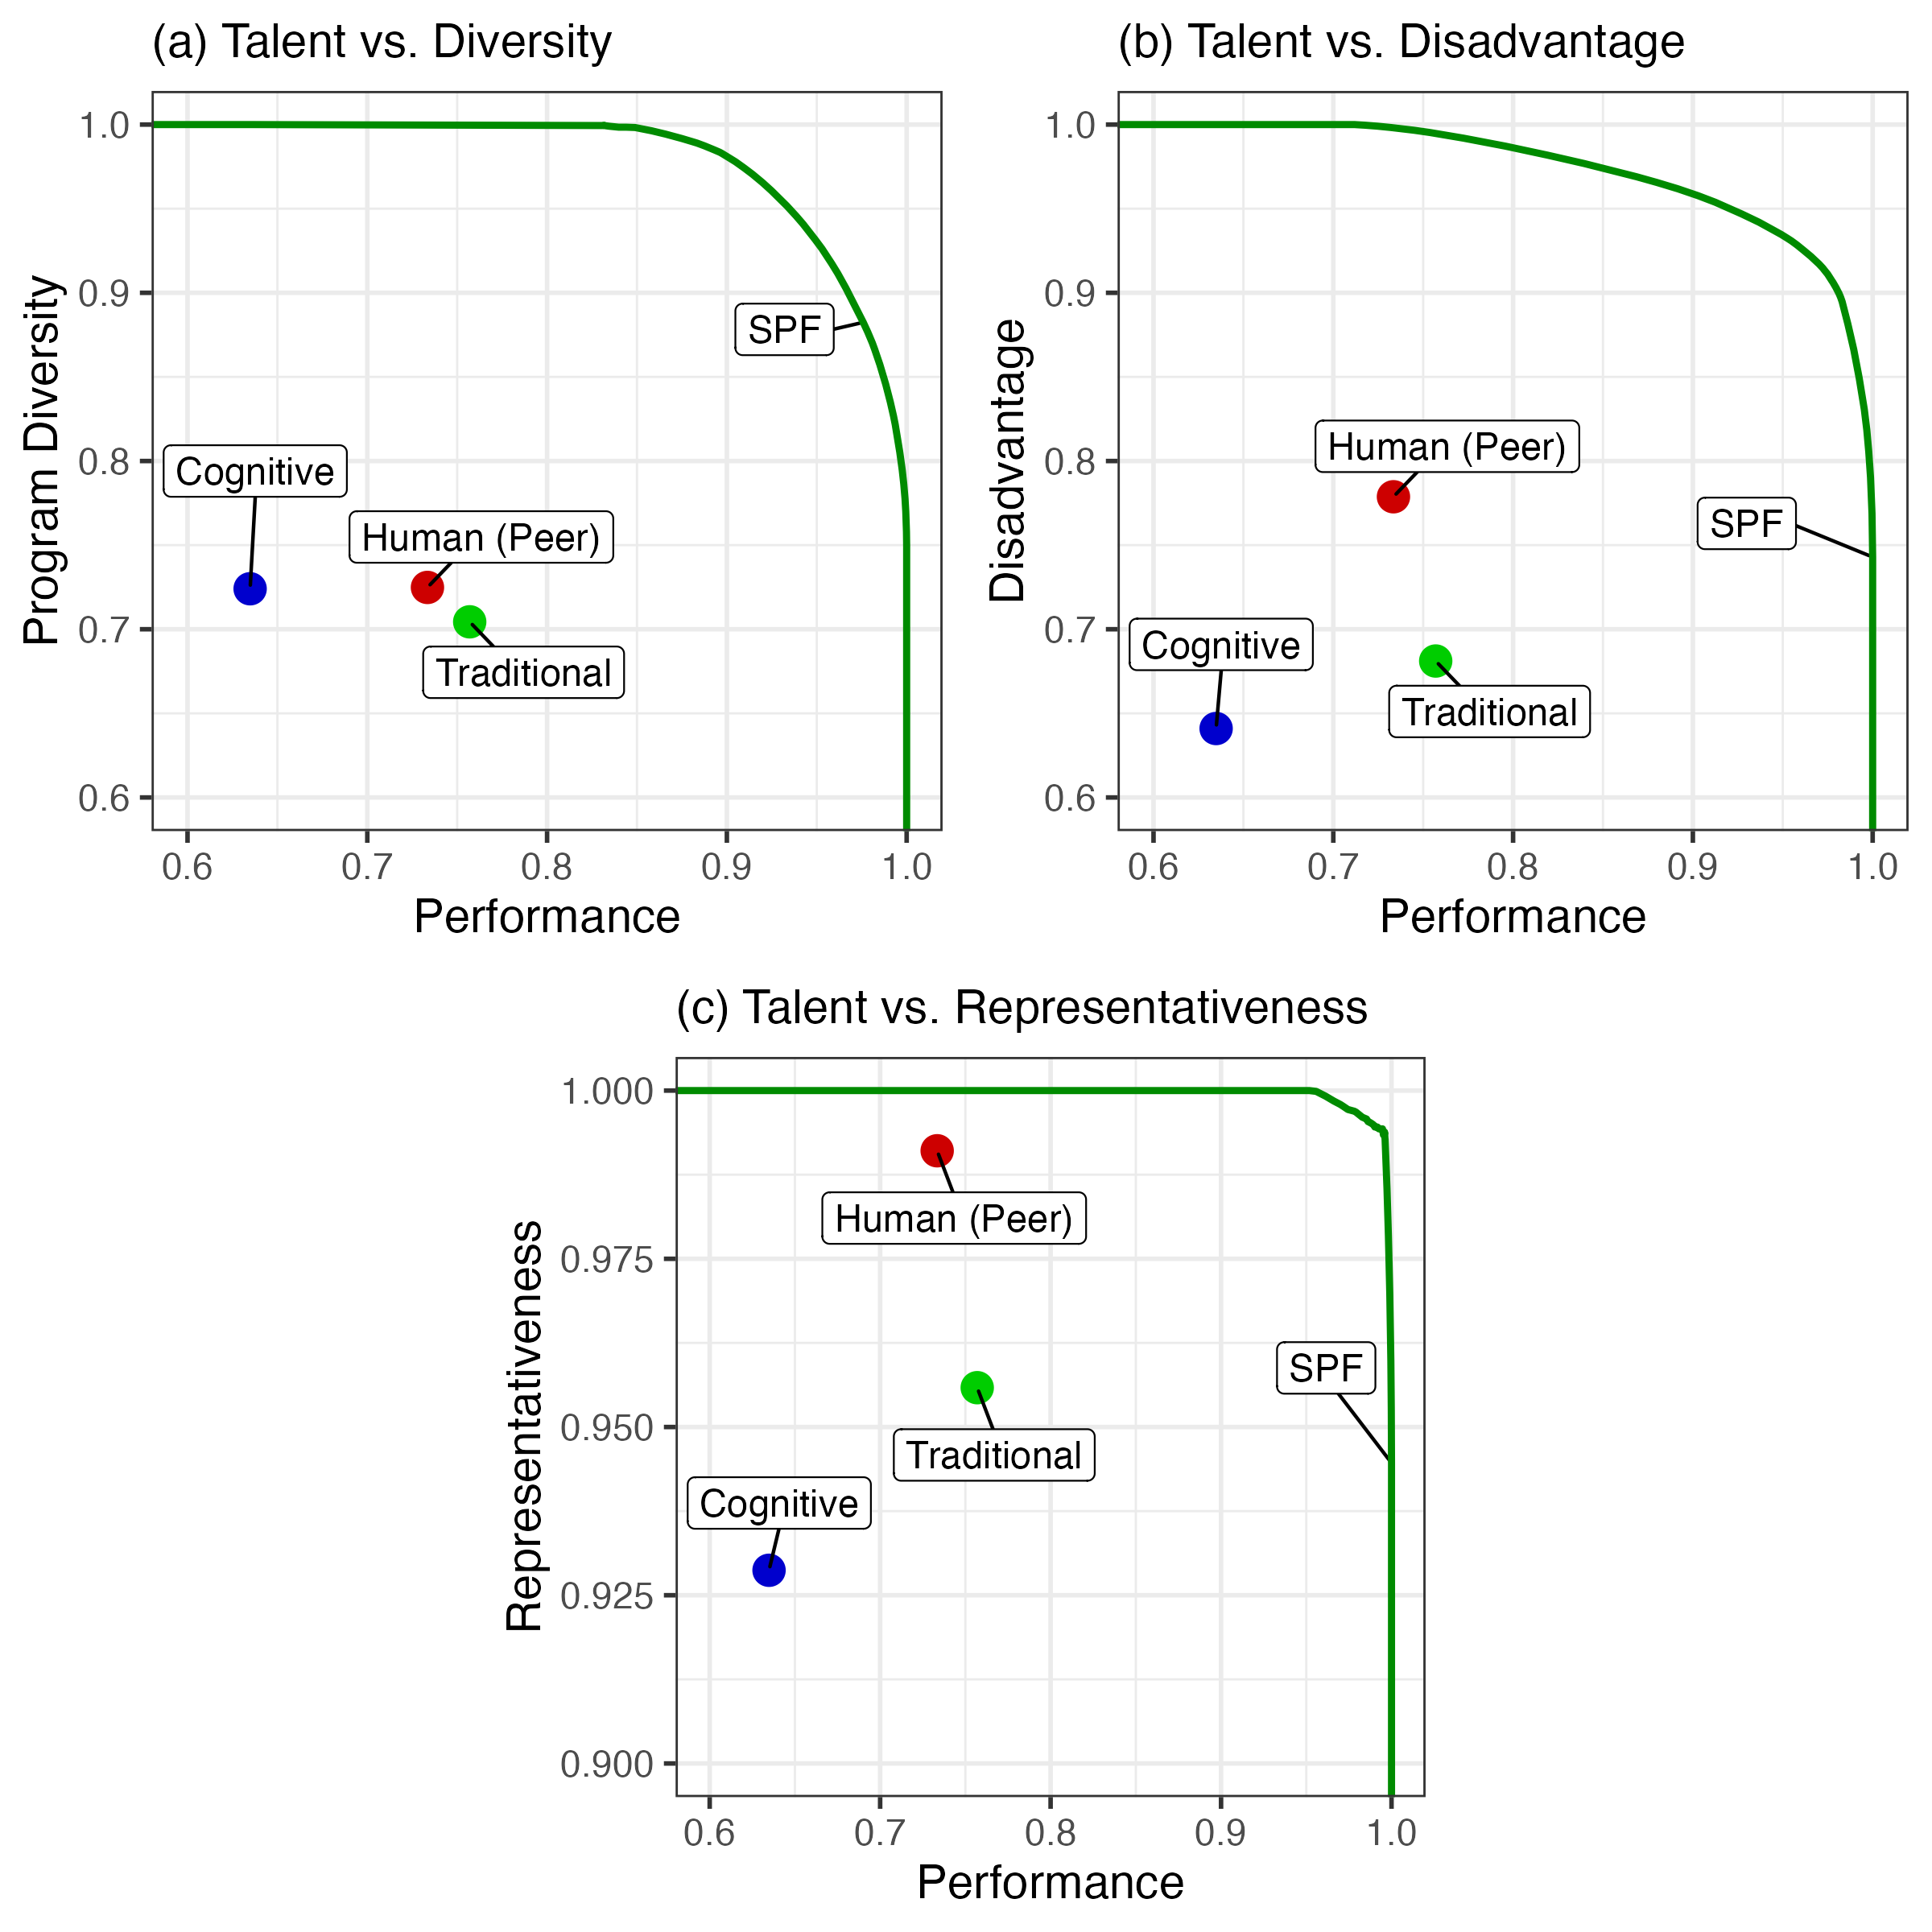
\includegraphics[width=\textwidth]{spf/alt_screening_performance.png} 
    \caption{This figure displays various SPF estimates for the  finalist cohort using the program's notion of diversity, a `disadvantage' notion of diversity (drawn from the `contextualising applications' theme in Chapter \ref{ch:diversity}), and a `representativeness' notion of diversity (i.e., Prototype \ref{fig:representativeness}). The y-axes represent diversity scores while the x-axes represent average cohort performance. The green curves are our estimates of three alternative Cycle 2021 SPFs, which are estimates the upper bound of diversity that is achievable at every level of cohort performance. Each dot represents the performance and diversity of cohorts had they been selected using only cognitive ability (blue), a combination of written essay judgements and cognitive ability (aka a "traditional" score, which is green), and just peer review (red).} \label{fig:alt_screen}
    \end{figure}

\paragraph{Evaluating According to Alternate Notions of Diversity} A similar process can help organisations understand the practical implications of different kinds of preferences over types of diversity. While we isolate three themes relating to definitions of diversity in Chapter \ref{ch:diversity}, we note that the Rise program has a working understanding of what they mean by diversity, and did not wish to adopt any of these notions. In practice, Rise's diversity targets suggest both `representativeness' and `contextualising applications' (which they internally call `disadvantage' or `boostability', variously) as important to their consideration of diversity, while `different perspectives' does not appear in their decision-making process. Thus, Figure \ref{fig:alt_screen} also depicts results using two alternative notions of diversity based only on the disadvantage and representativeness portions of the Rise targets. The disadvantage diversity score puts maximal weight on representing those from various historically disadvantaged groups (e.g., being first-generation, poor, or female) while the representativeness diversity score only uses proportional targets that match the demographic distribution of the applicants. Evaluating each alternative selection method indicates that, while selecting on peer judgements or the traditional score both do substantially better than using cognitive ability alone on the talent dimension, using the peer score is by far the highest performing on both disadvantage and representativeness.

\section{Conclusion} \label{sec:conclusion}
While Chapter \ref{ch:diversity} focused on the theoretical and empirical aspects of diversity, this chapter has focused on the practical implications of diversity in selection. In doing so, we have introduced the notion of a selection possibilities frontier via a simple model of diverse talent selection, have implemented Prototype \ref{fig:diversity} as an in-process DST, and have demonstrated its use in practice. Analysing decision-making with and without our DST, we have shown that Rise selects talented and more diverse cohorts when given access to our SPF-based DST. To explain why, we showed that the diverse talent selection problem is $\mathbf{NP}$-hard and augmented our model with a notion of complexity costs; this new model predicts that organisations who are better and more cheaply able to approximate the frontier should find themselves closer to it. 

Finally, we have also shown that the SPF can be used \emph{ex-post} to compare the diversity tradeoffs of alternative talent measures, evaluate alternative selection and screening approaches, and evaluate according to alternate notions of diversity. 

In an age of rapidly expanding interest in selecting from diverse talent pools (signaled by the growth of DEI), this chapter has wide-ranging policy implications. First, the chapter suggests that organisations will face extreme difficulty executing on their diversity goals unless they are willing to adopt more sophisticated selection technology. Second, this chapter contributes methods that are particularly useful for assessing the diversity impacts of alternative merit-based selection strategies. This extends beyond selection to related contexts like hiring, where not appropriately considering the diversity implications of selection strategies can result in lawsuits, and U.S. university admissions non-merit-based selection has become a legal gray area despite university commitments to diversity. 



% % Figures and Tables Below
    
%     \newpage
%     \begin{figure}[!htb]
%     \centering
%         \caption{This figure depicts an example solution to an iteration of the selection problem with complexity induced search costs, which is described in Equation \ref{eq:objective}. As in Figure \ref{fig:model_spf}, the solid blue curve represents the SPF, the dotted blue curve represents the organisation's indifference curve corresponding to the highest achievable utility without search costs, and the blue dot represents the diversity and performance of the first-best solution. Additionally, the solid red curve represents the accessible frontier with optimal search, the dotted red curve that represents the highest achievable utility with search costs, and the red dot that represents the diversity and performance of the optimal cohort with search costs (i.e. the second-best solution).}\label{fig:model_complex}
%       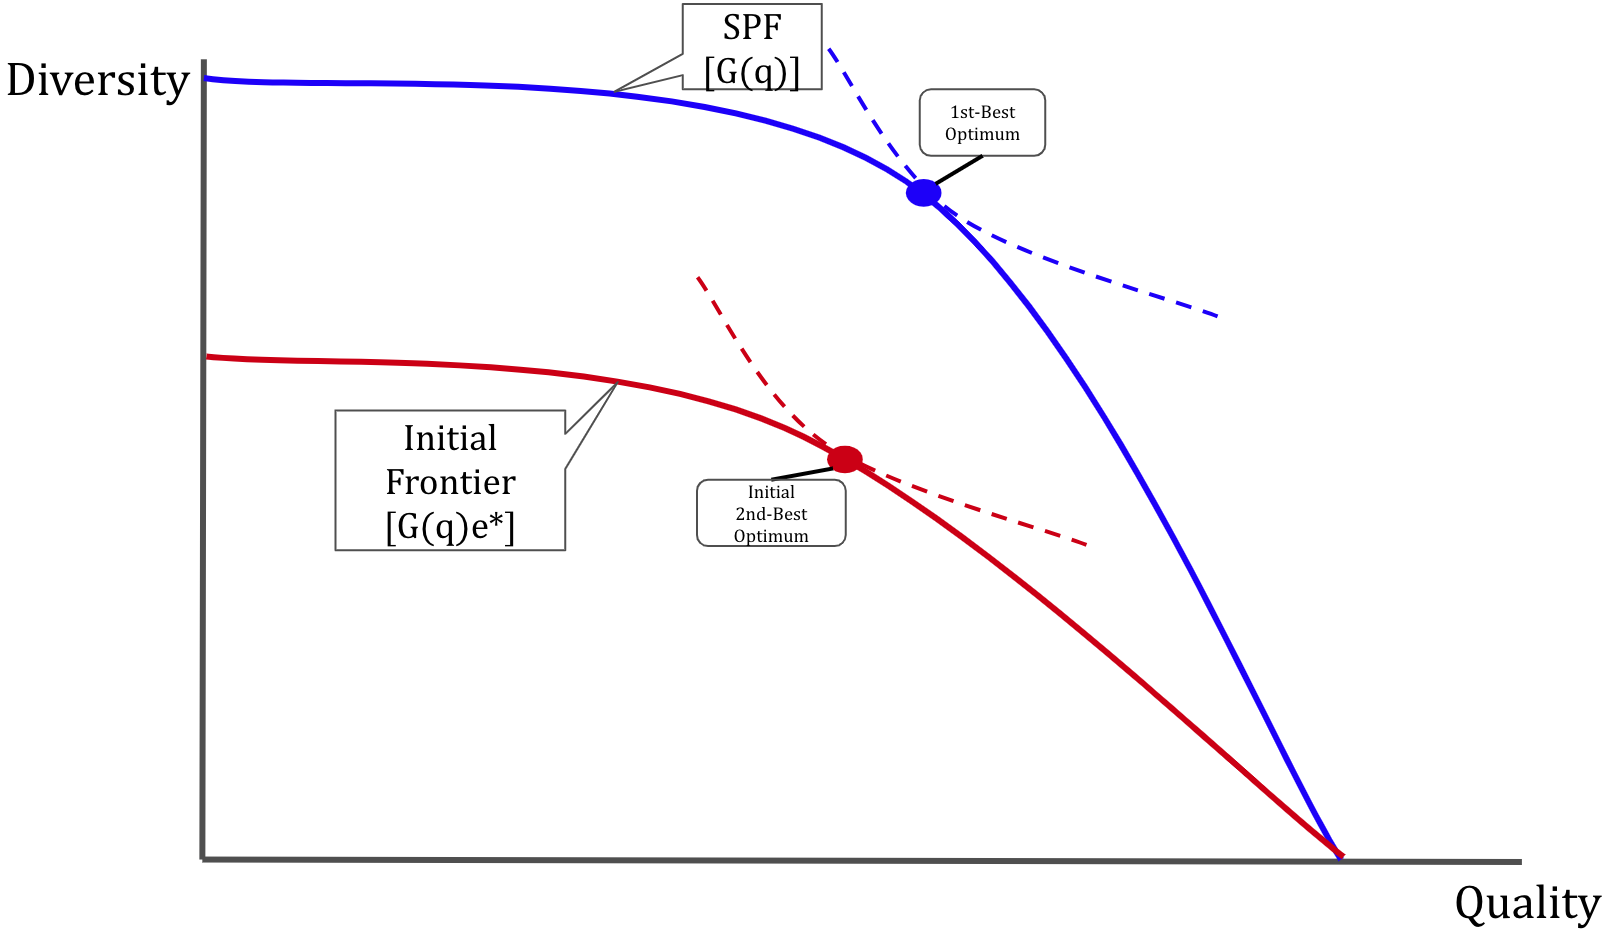
\includegraphics[width=1\textwidth,height=\textheight,keepaspectratio]{spf/model_complex.png} 
%     \end{figure}
    
%     \newpage
%     \begin{figure}[!htb]
%     \centering
%         \caption{This figure depicts an example solution to an iteration of the selection problem with complexity induced search costs, which is described in Equation \ref{eq:objective}. As in Figure \ref{fig:model_spf}, the solid blue curve represents the SPF, the dotted blue curve represents the organisation's indifference curve corresponding to the highest achievable utility without search costs, and the blue dot represents the diversity and performance of the first-best solution. And, as in \ref{fig:model_spf}, the solid red curve represents the accessible frontier with optimal search, the dotted red curve that represents the highest achievable utility with search costs, and the red dot that represents the diversity and performance of the second-best cohort with poor search technology (i.e. high $\alpha$). And, the green curves and dot represent the SPF estimate that is accessible with an improved search technology and new second-best solution, respectively. The difference between the initial second-best solution and the new solution is a graphical representation of the implications of the comparative static signed in Equation \ref{eq:comp_stat} ($\frac{\partial e^*}{\partial \alpha}$).}\label{fig:model_spf_est}
%       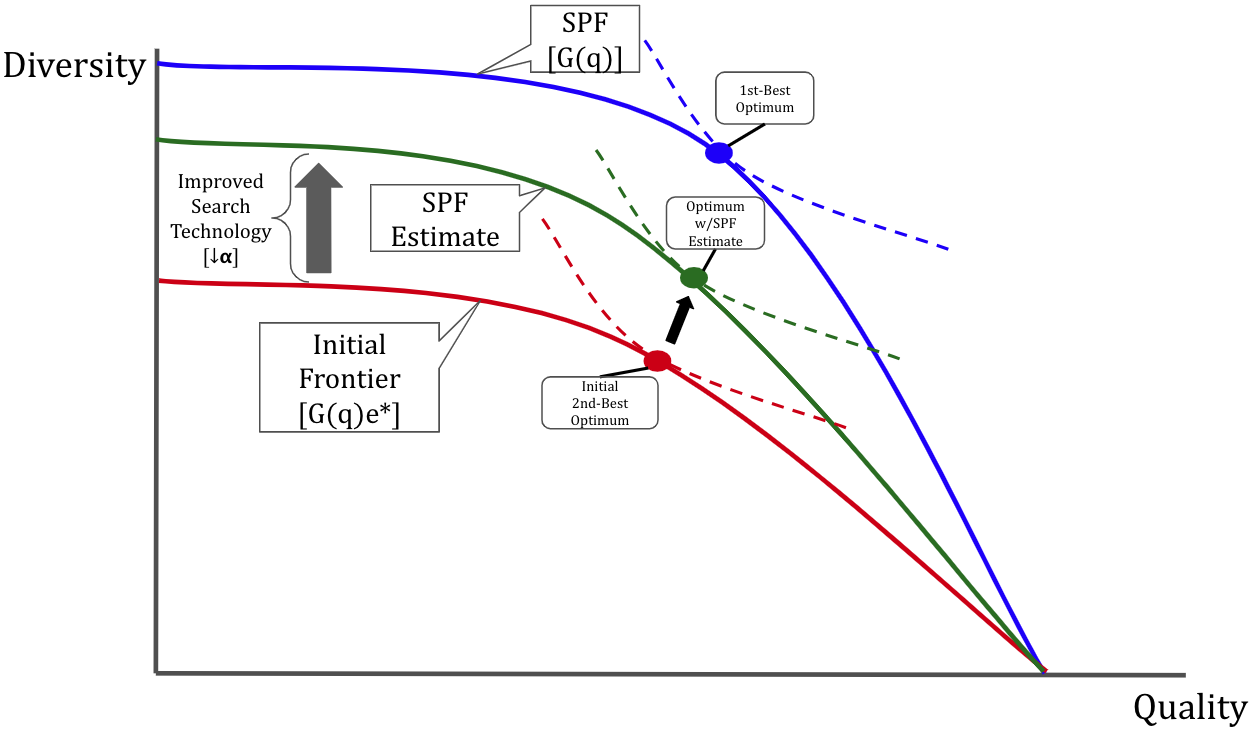
\includegraphics[width=1\textwidth,height=\textheight,keepaspectratio]{spf/model_spf_est.png}
%     \end{figure}
    
    
%     \newpage
%     \null %The \null -> \vfill -> figure code -> \vfill code centers the figure vertically on the page
%     \vfill
%     \begin{center}
%     \begin{figure}[!htb]
%     \centering
%         \caption{This figure schematizes the key elements of the talent investment program's data collection and selection process. }\label{fig:design}
%       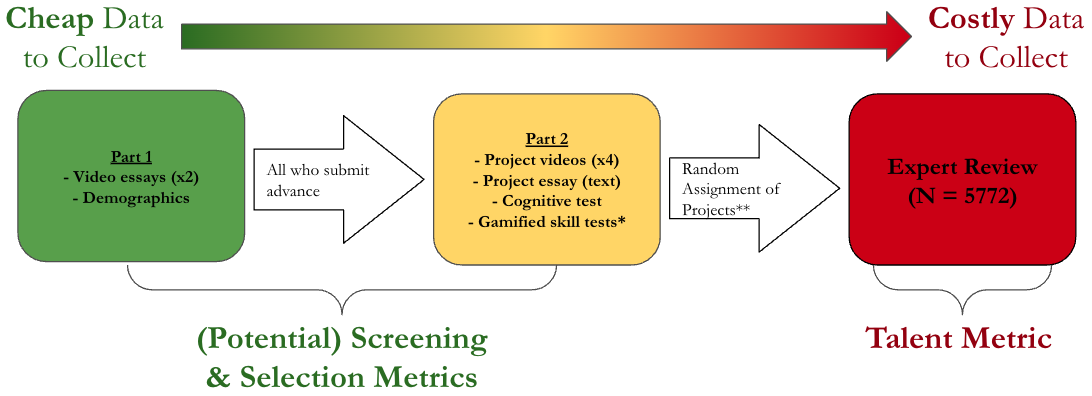
\includegraphics[width=\textwidth,height=\textheight,keepaspectratio]{spf/selection_design_schematic.png} 
%     \end{figure}
%     \end{center}
%     \vfill
    
    
%     \newpage
    
%     \begin{figure}[!htb]
%     \centering
%         \caption{Distribution of Applicant Countries Data come from surveys completed by applicants. Data are pooled across all three application cohorts. Overall applicants come from 153 different countries. The distribution of proportions of applicants by country in this figure are limited to the 50 countries from which there were the most applicants. The top 5 countries are labeled on the figure.  }\label{fig:country_dist_all}
%       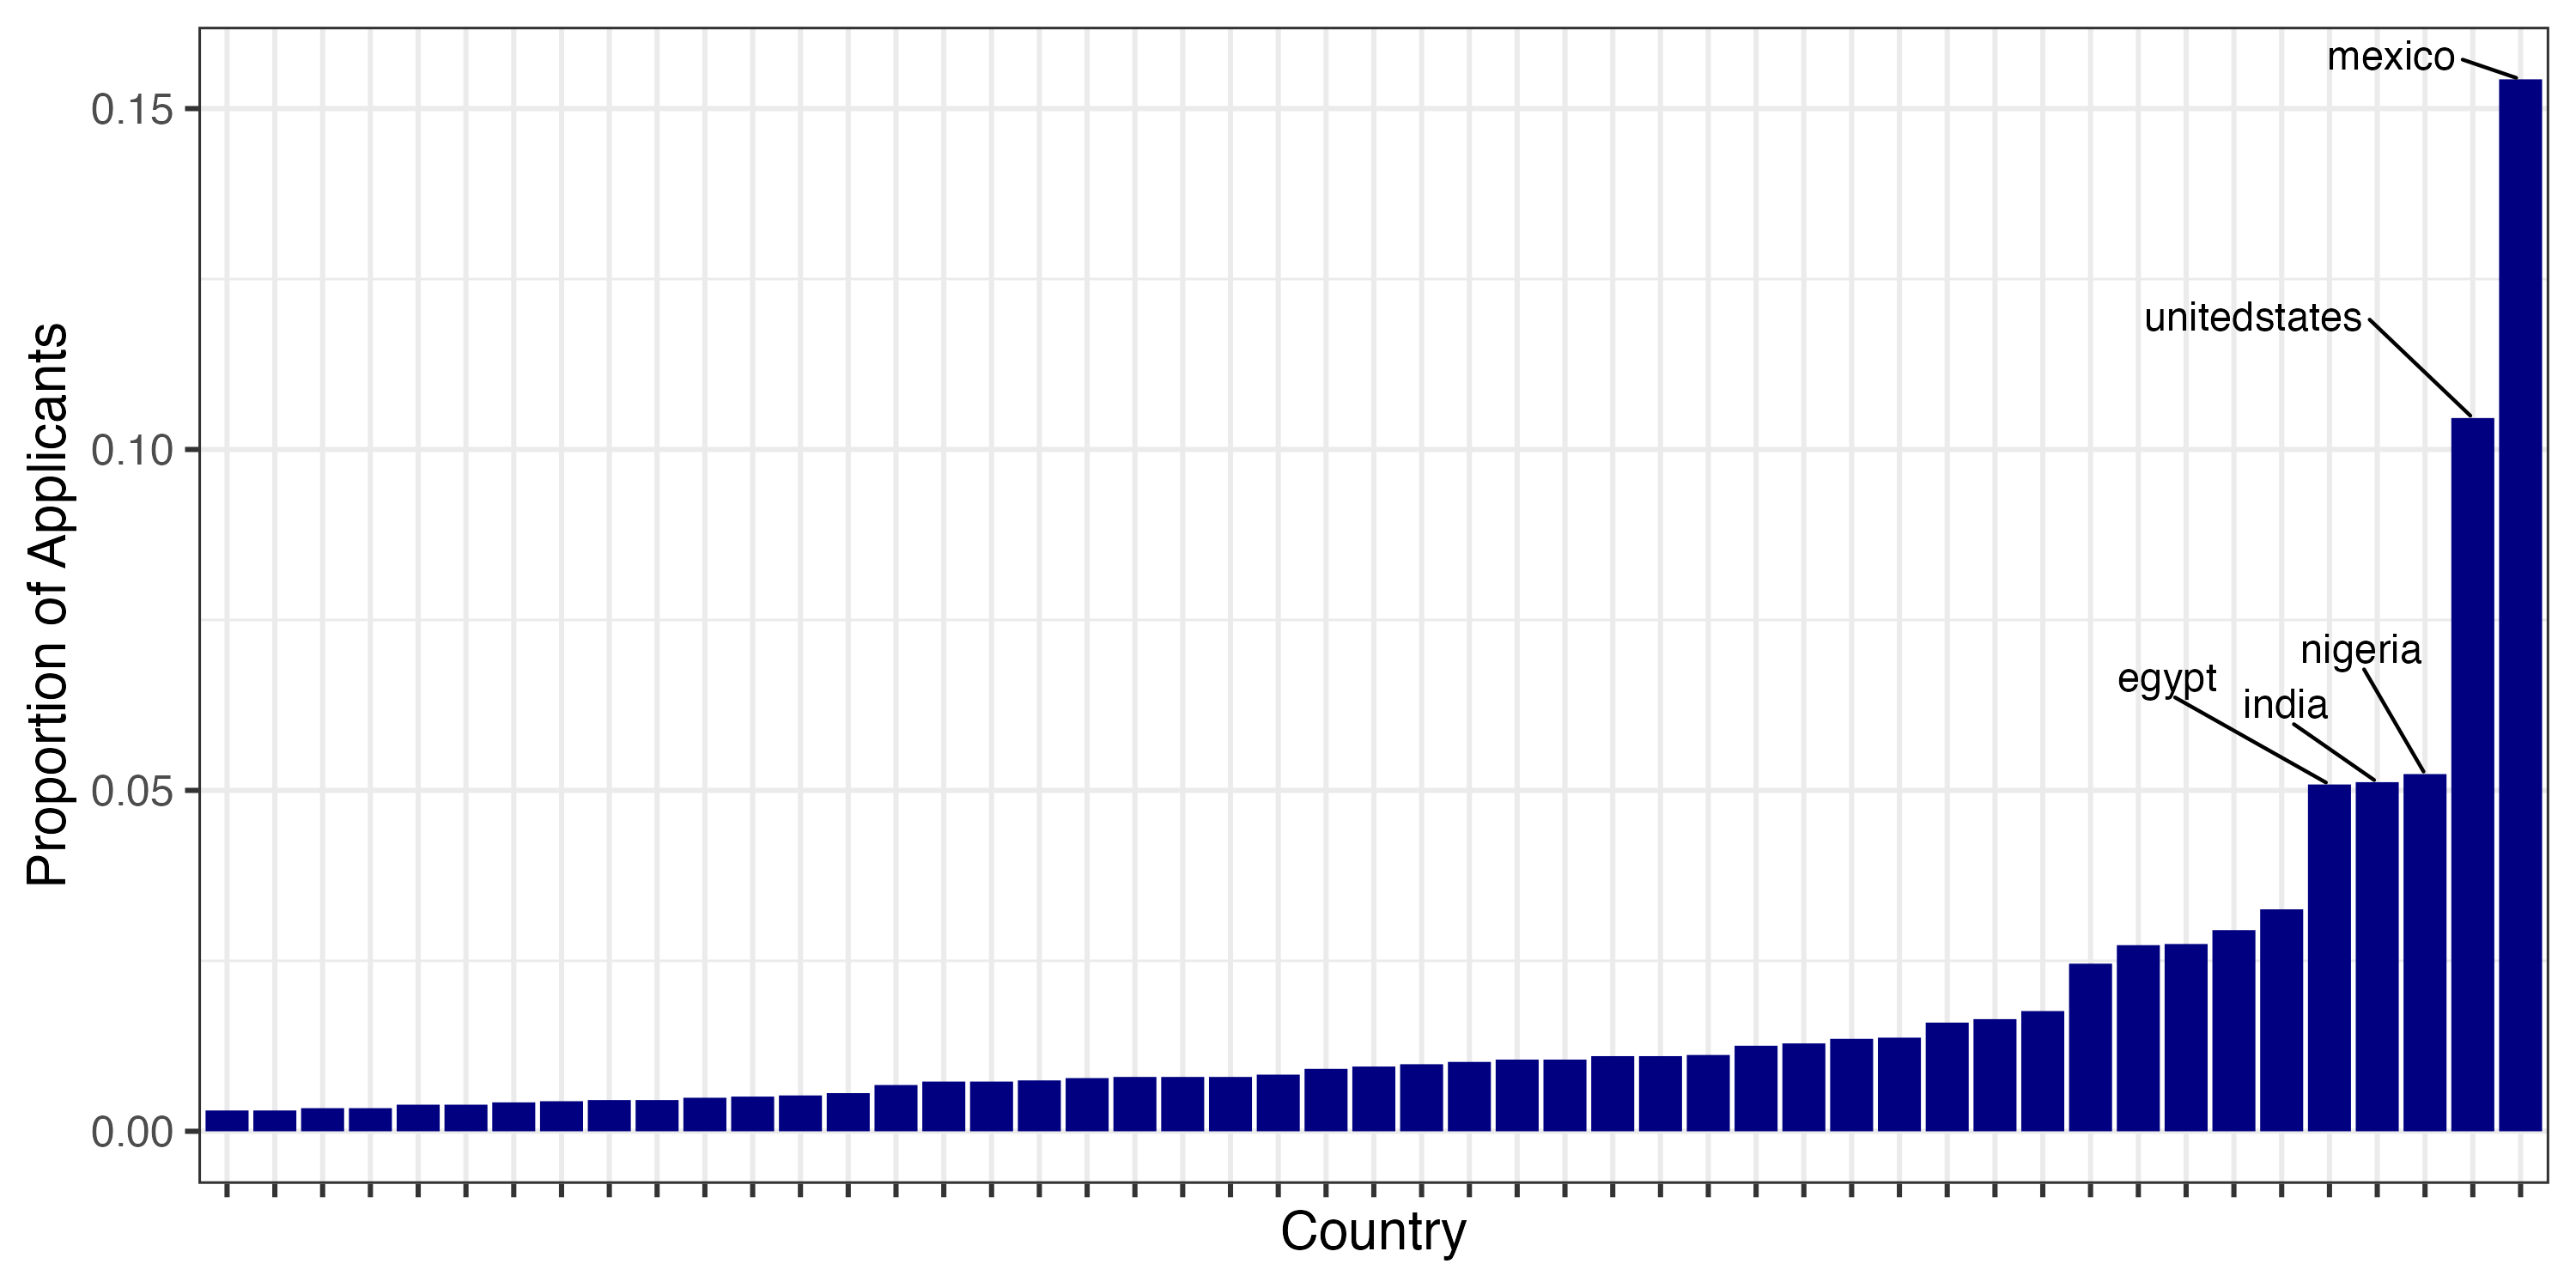
\includegraphics[width=.9\textwidth]{spf/candidate_countries.png} 
%     \end{figure}
    
    
%     \begin{figure}[!htb]
%         \centering
%         \caption{Distributions of Applicant Project Topics and Reviewer Expertise. Data come from surveys completed by applicants. Data are pooled across all three application cohorts. Panel (\ref{subfig:app_proj_topics}) depicts the proportion of all applicant projects in each topic category. Panel (\ref{subfig:rev_expertise}) depicts the proportion of project reviewers with each category of expertise.} \label{fig:topic_expertise_dist}
%         \begin{subfigure}[t]{\textwidth}
%             \centering
%                     \caption{Applicant Project Topics} \label{subfig:app_proj_topics}
%             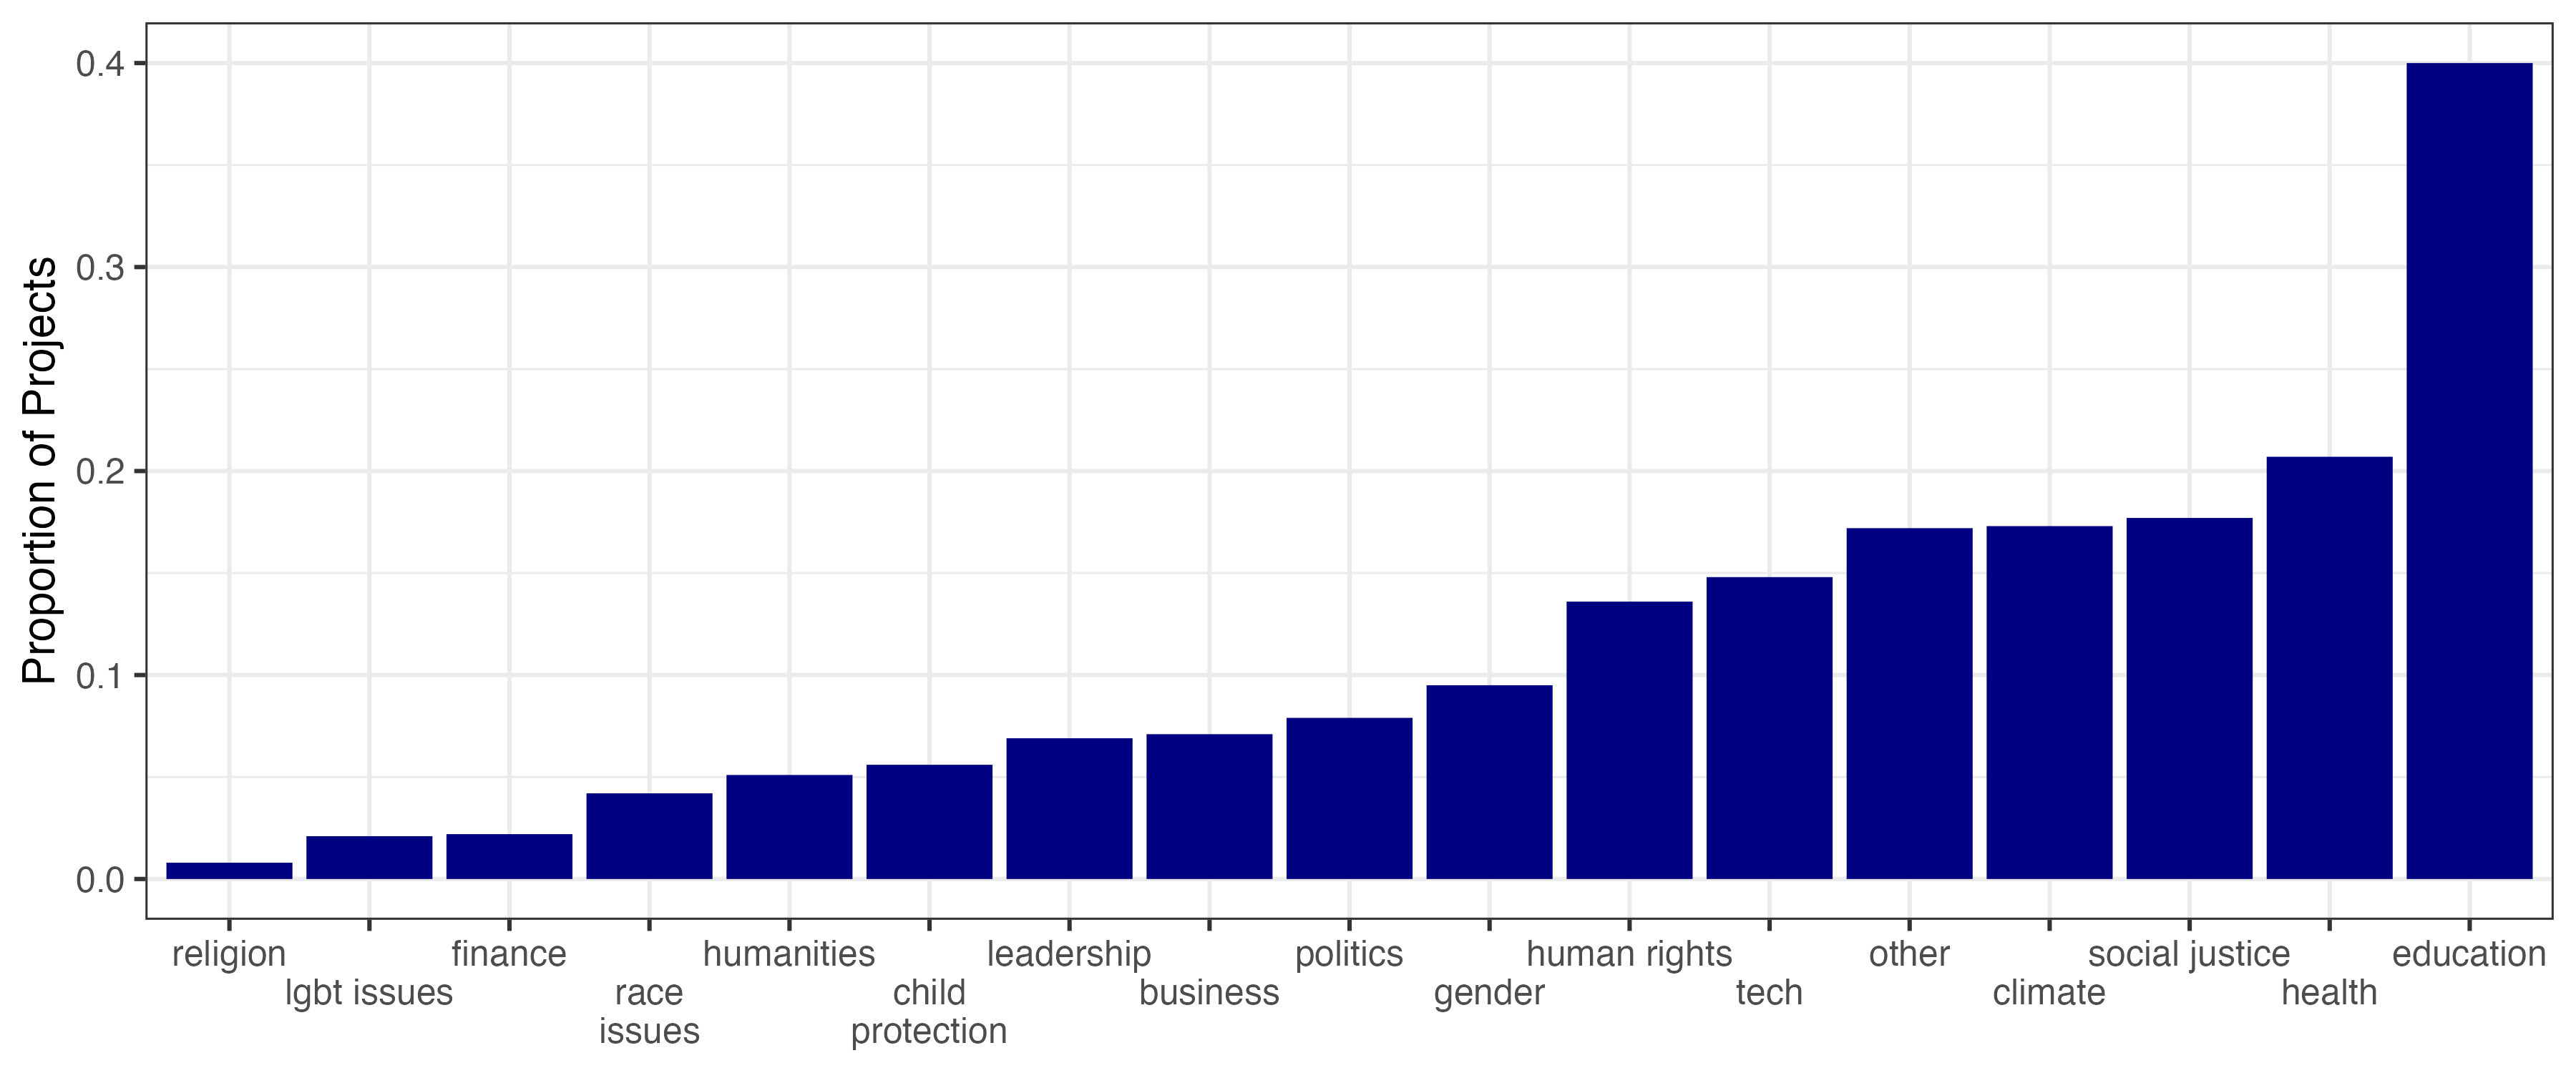
\includegraphics[width=\linewidth]{spf/applicant_project_topics.png} 
%         \end{subfigure}
%         \hfill
%         \vspace{1em}
%         \begin{subfigure}[t]{\textwidth}
%             \centering
%                    \caption{Reviewer Areas of Expertise} \label{subfig:rev_expertise}
%             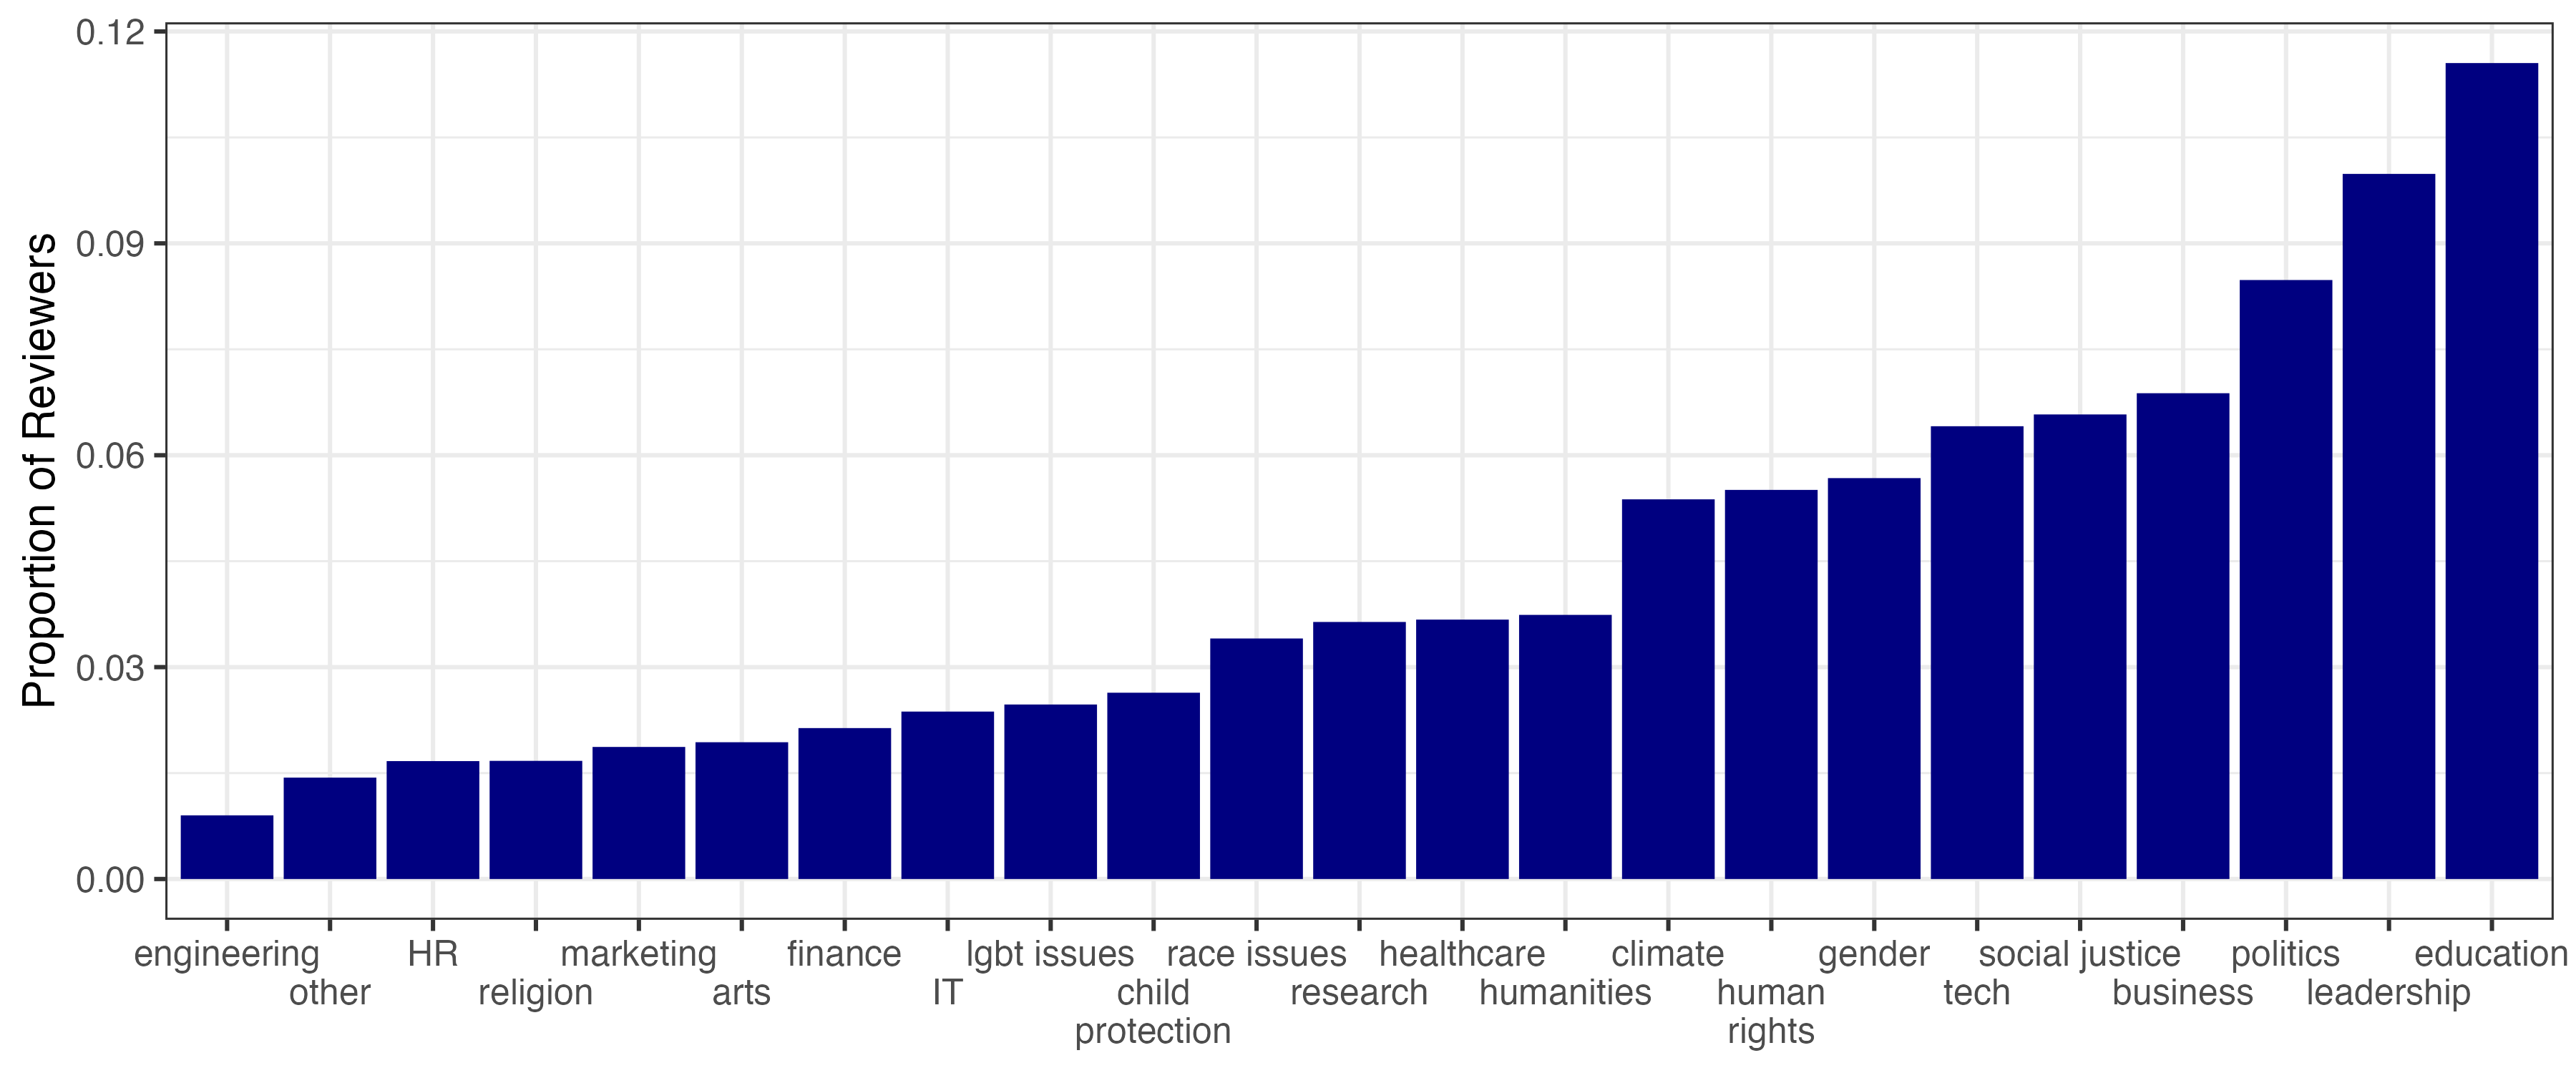
\includegraphics[width=\linewidth]{spf/reviewer_expertise.png} 
%         \end{subfigure}
%     \end{figure}
    
    
%     \begin{figure}[!htb]
%         \centering
%         \caption{Distributions of Reviewer Industries and Organisations (Cycle 1). Data come from surveys completed by applicants. Data come from application cycle 1 only (industry and organisation information were not collected for the in cycles 2 and 3). Panel (\ref{subfig:rev_industries}) depicts the proportion of all project reviewers by industries. Unfortunately, industries were not categorized using standard codes, but the categories are decipherable. Panel (\ref{subfig:rev_orgs}) depicts the proportion of project reviewers from each organisation that referred them. The top two most common referring organisations make up 46\% of all expert reviewers, and the labels on them have been redacted to maintain the program's anonymity. }
%         \begin{subfigure}[t]{\textwidth}
%             \centering
%                     \caption{Industries} \label{subfig:rev_industries}
%             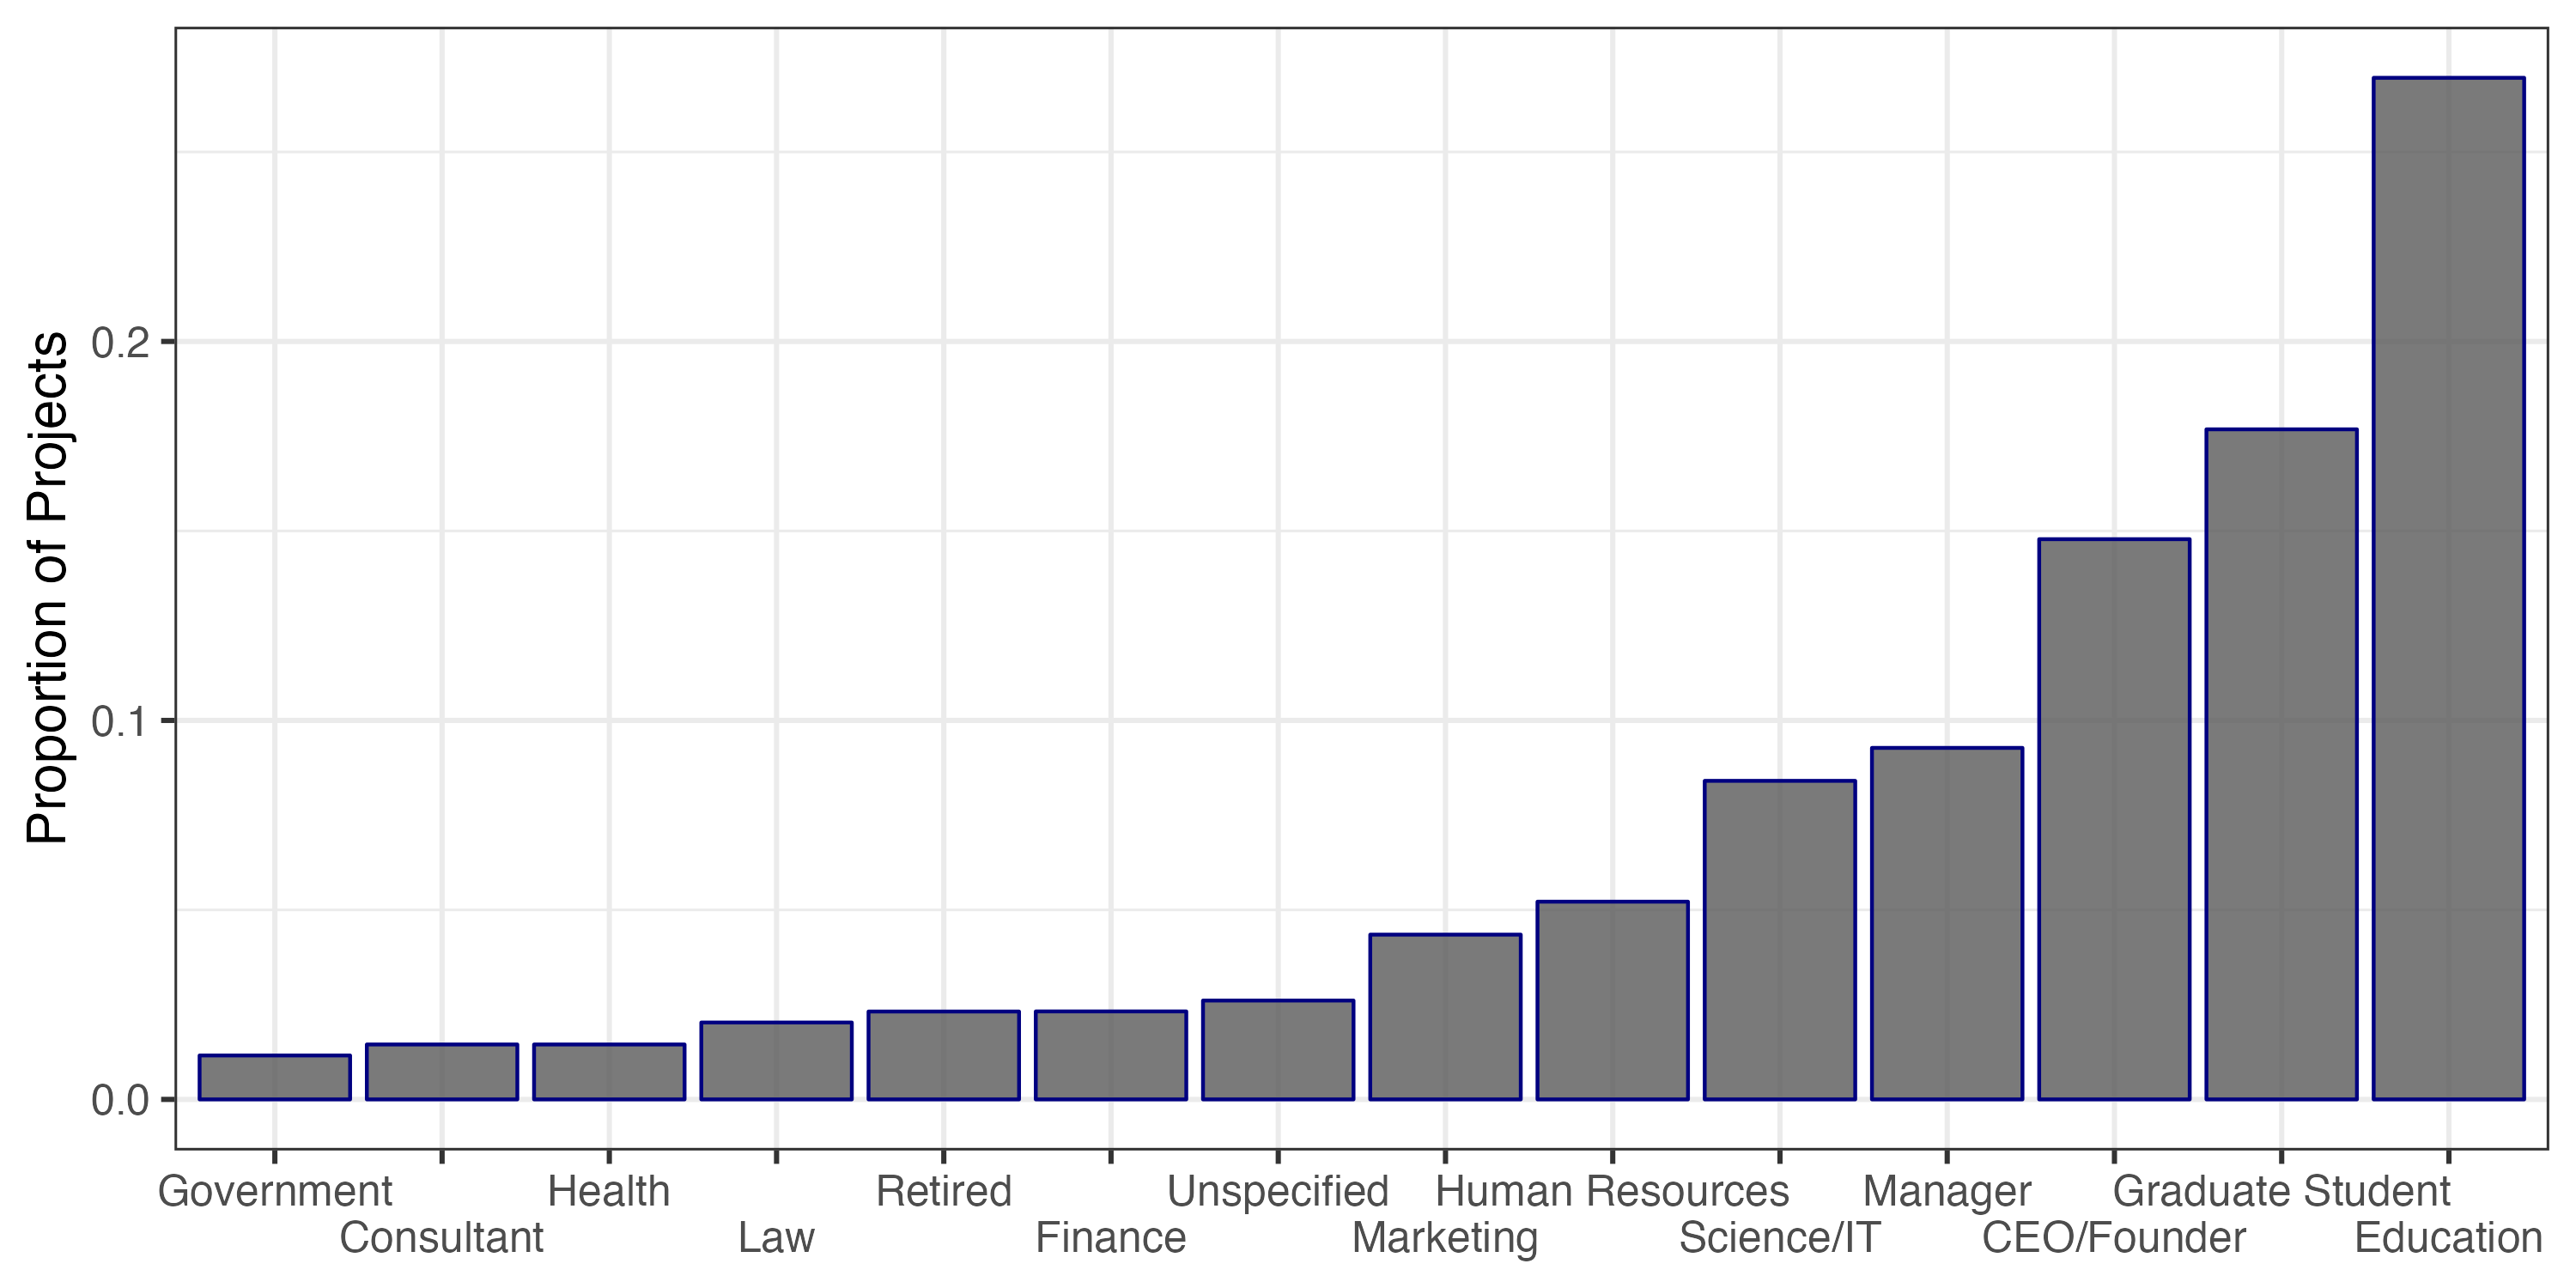
\includegraphics[width=\linewidth]{spf/project_reviewer_industries.png} 
%         \end{subfigure}
%         \hfill
%         \vspace{1em}
%         \begin{subfigure}[t]{\textwidth}
%             \centering
%                    \caption{Organisations (Top 2 Labeled)} \label{subfig:rev_orgs}
%             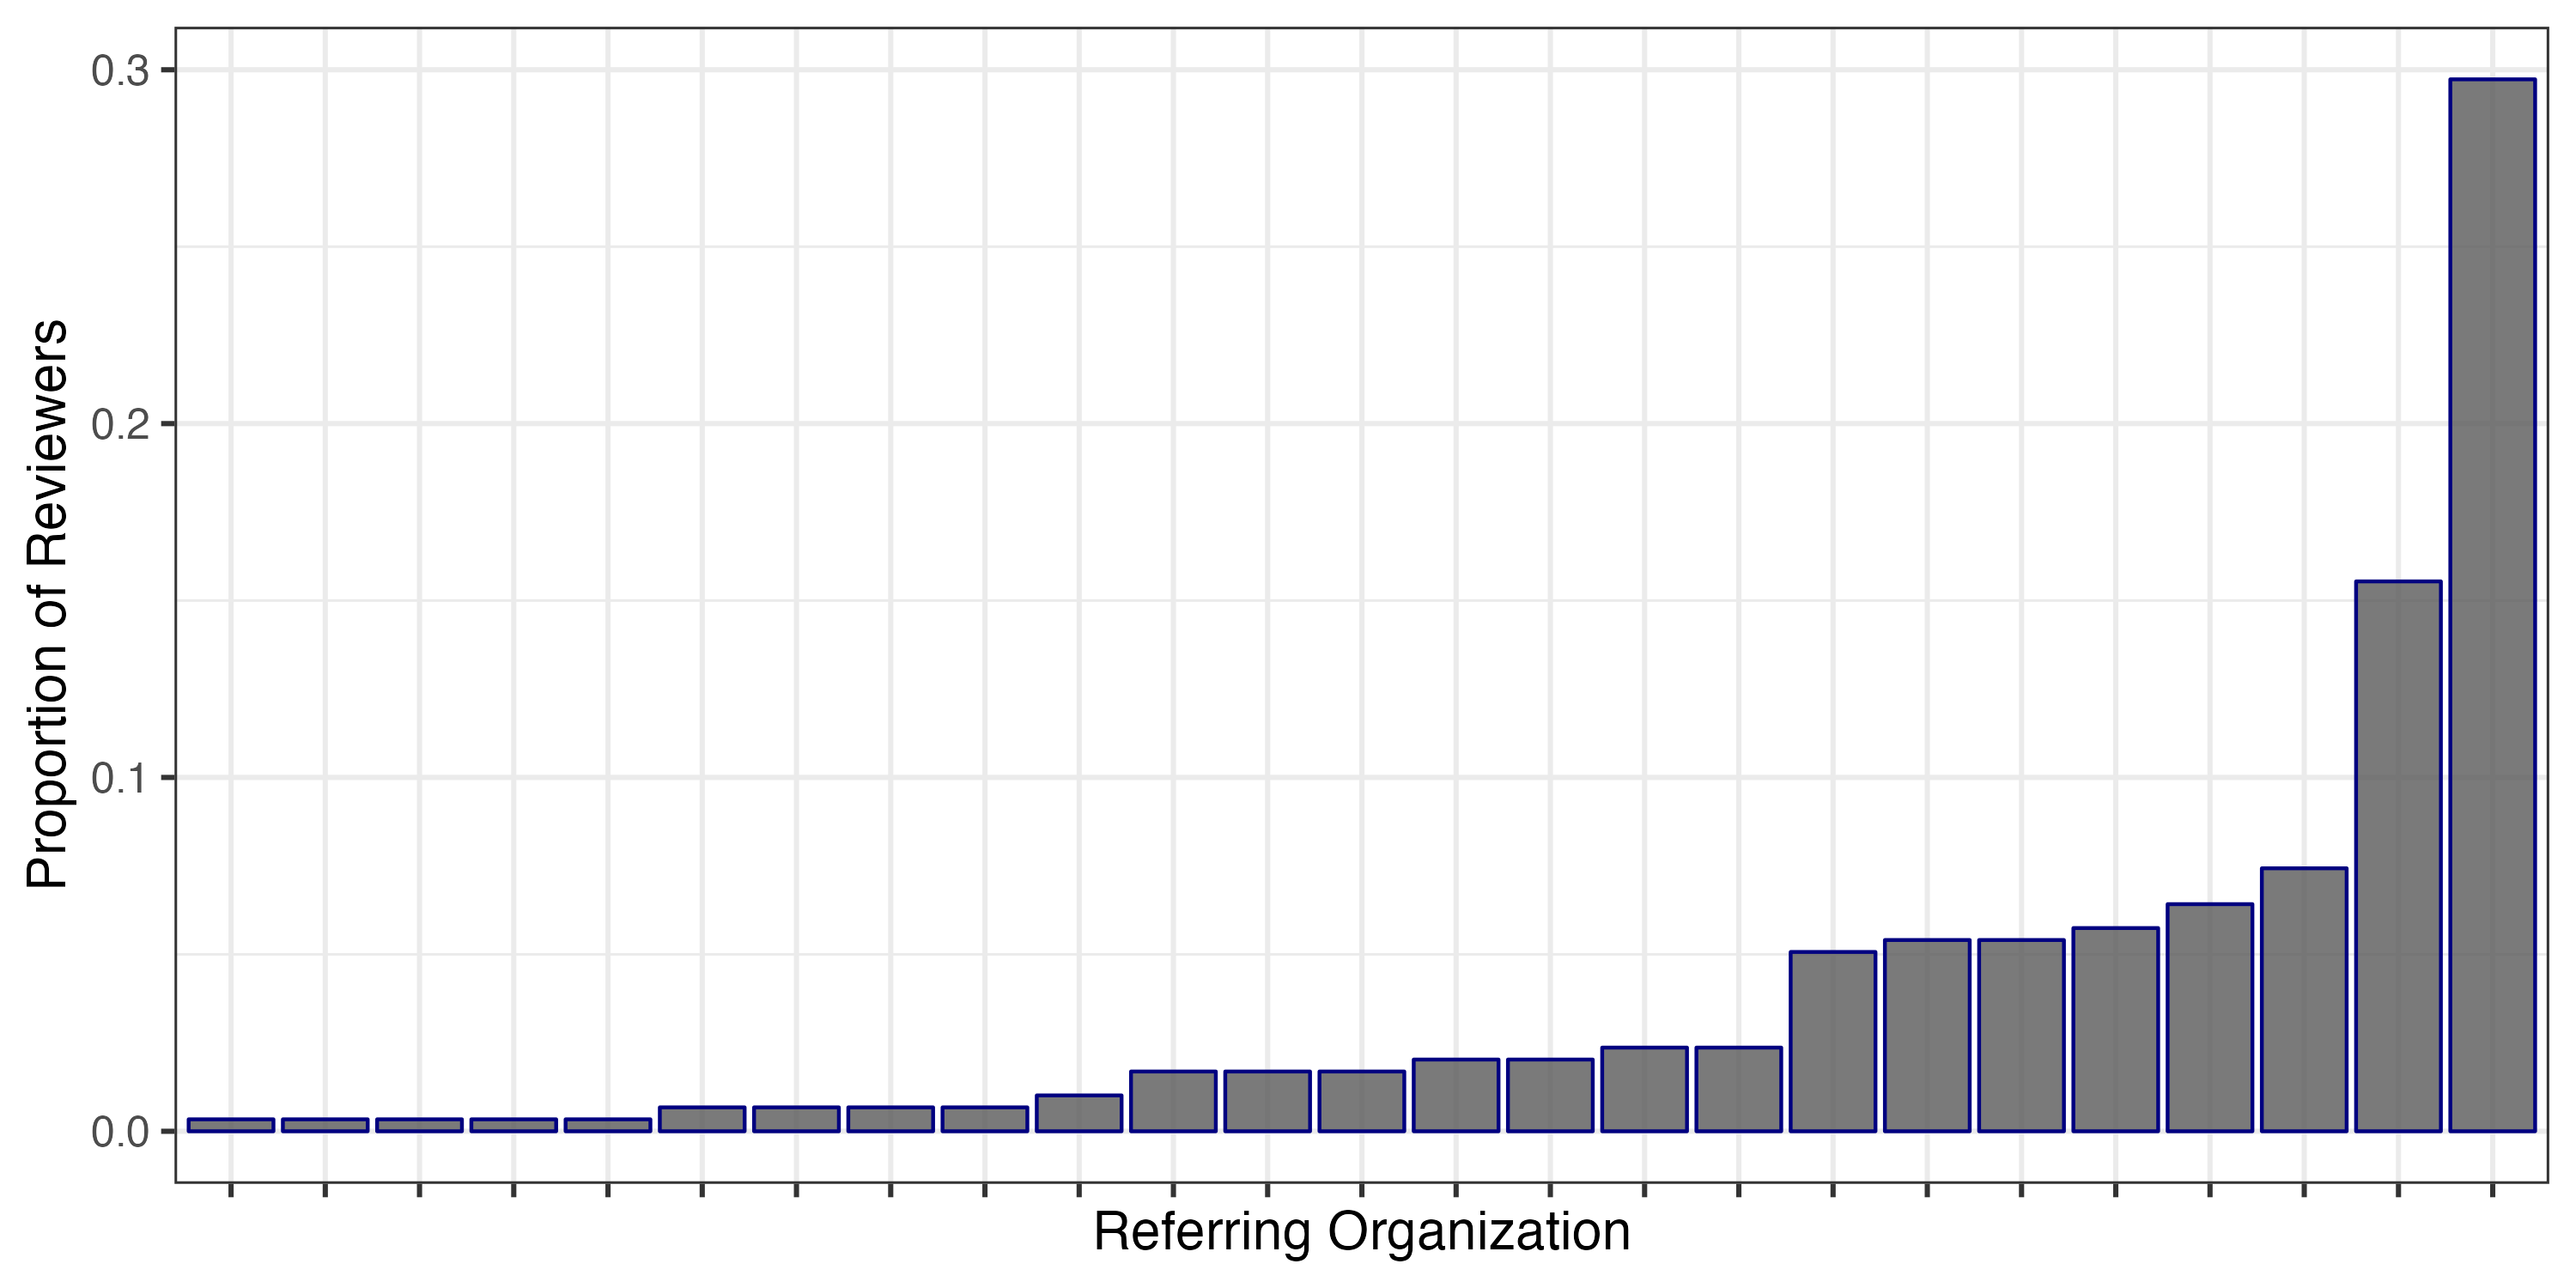
\includegraphics[width=\linewidth]{spf/project_reviewer_affiliations.png} 
%         \end{subfigure}
%     \end{figure}

    
%     \newpage
%     \begin{figure}[!htb]
%     \centering
%         \caption{This figure displays the SPF we estimate for the cycle 3 finalist cohort. The y-axis represents the diversity score while the x-axis represents average cohort performance (i.e. project scores). The green curve is our estimate of the cycle 3 SPF, which represents the upper bound of diversity that is achievable at every level of cohort performance.The red dots depict the actual level of diversity and performance of the finalists that were selected in cycles 1-3, respectively. The diagonal dashed red line represents the distance in diversity-performance space between the cycle 2 cohort and the cycle 3 cohort. In cycle 3, there are no significant Pareto improvements on either diversity or performance. } \label{fig:spf_2023}
%       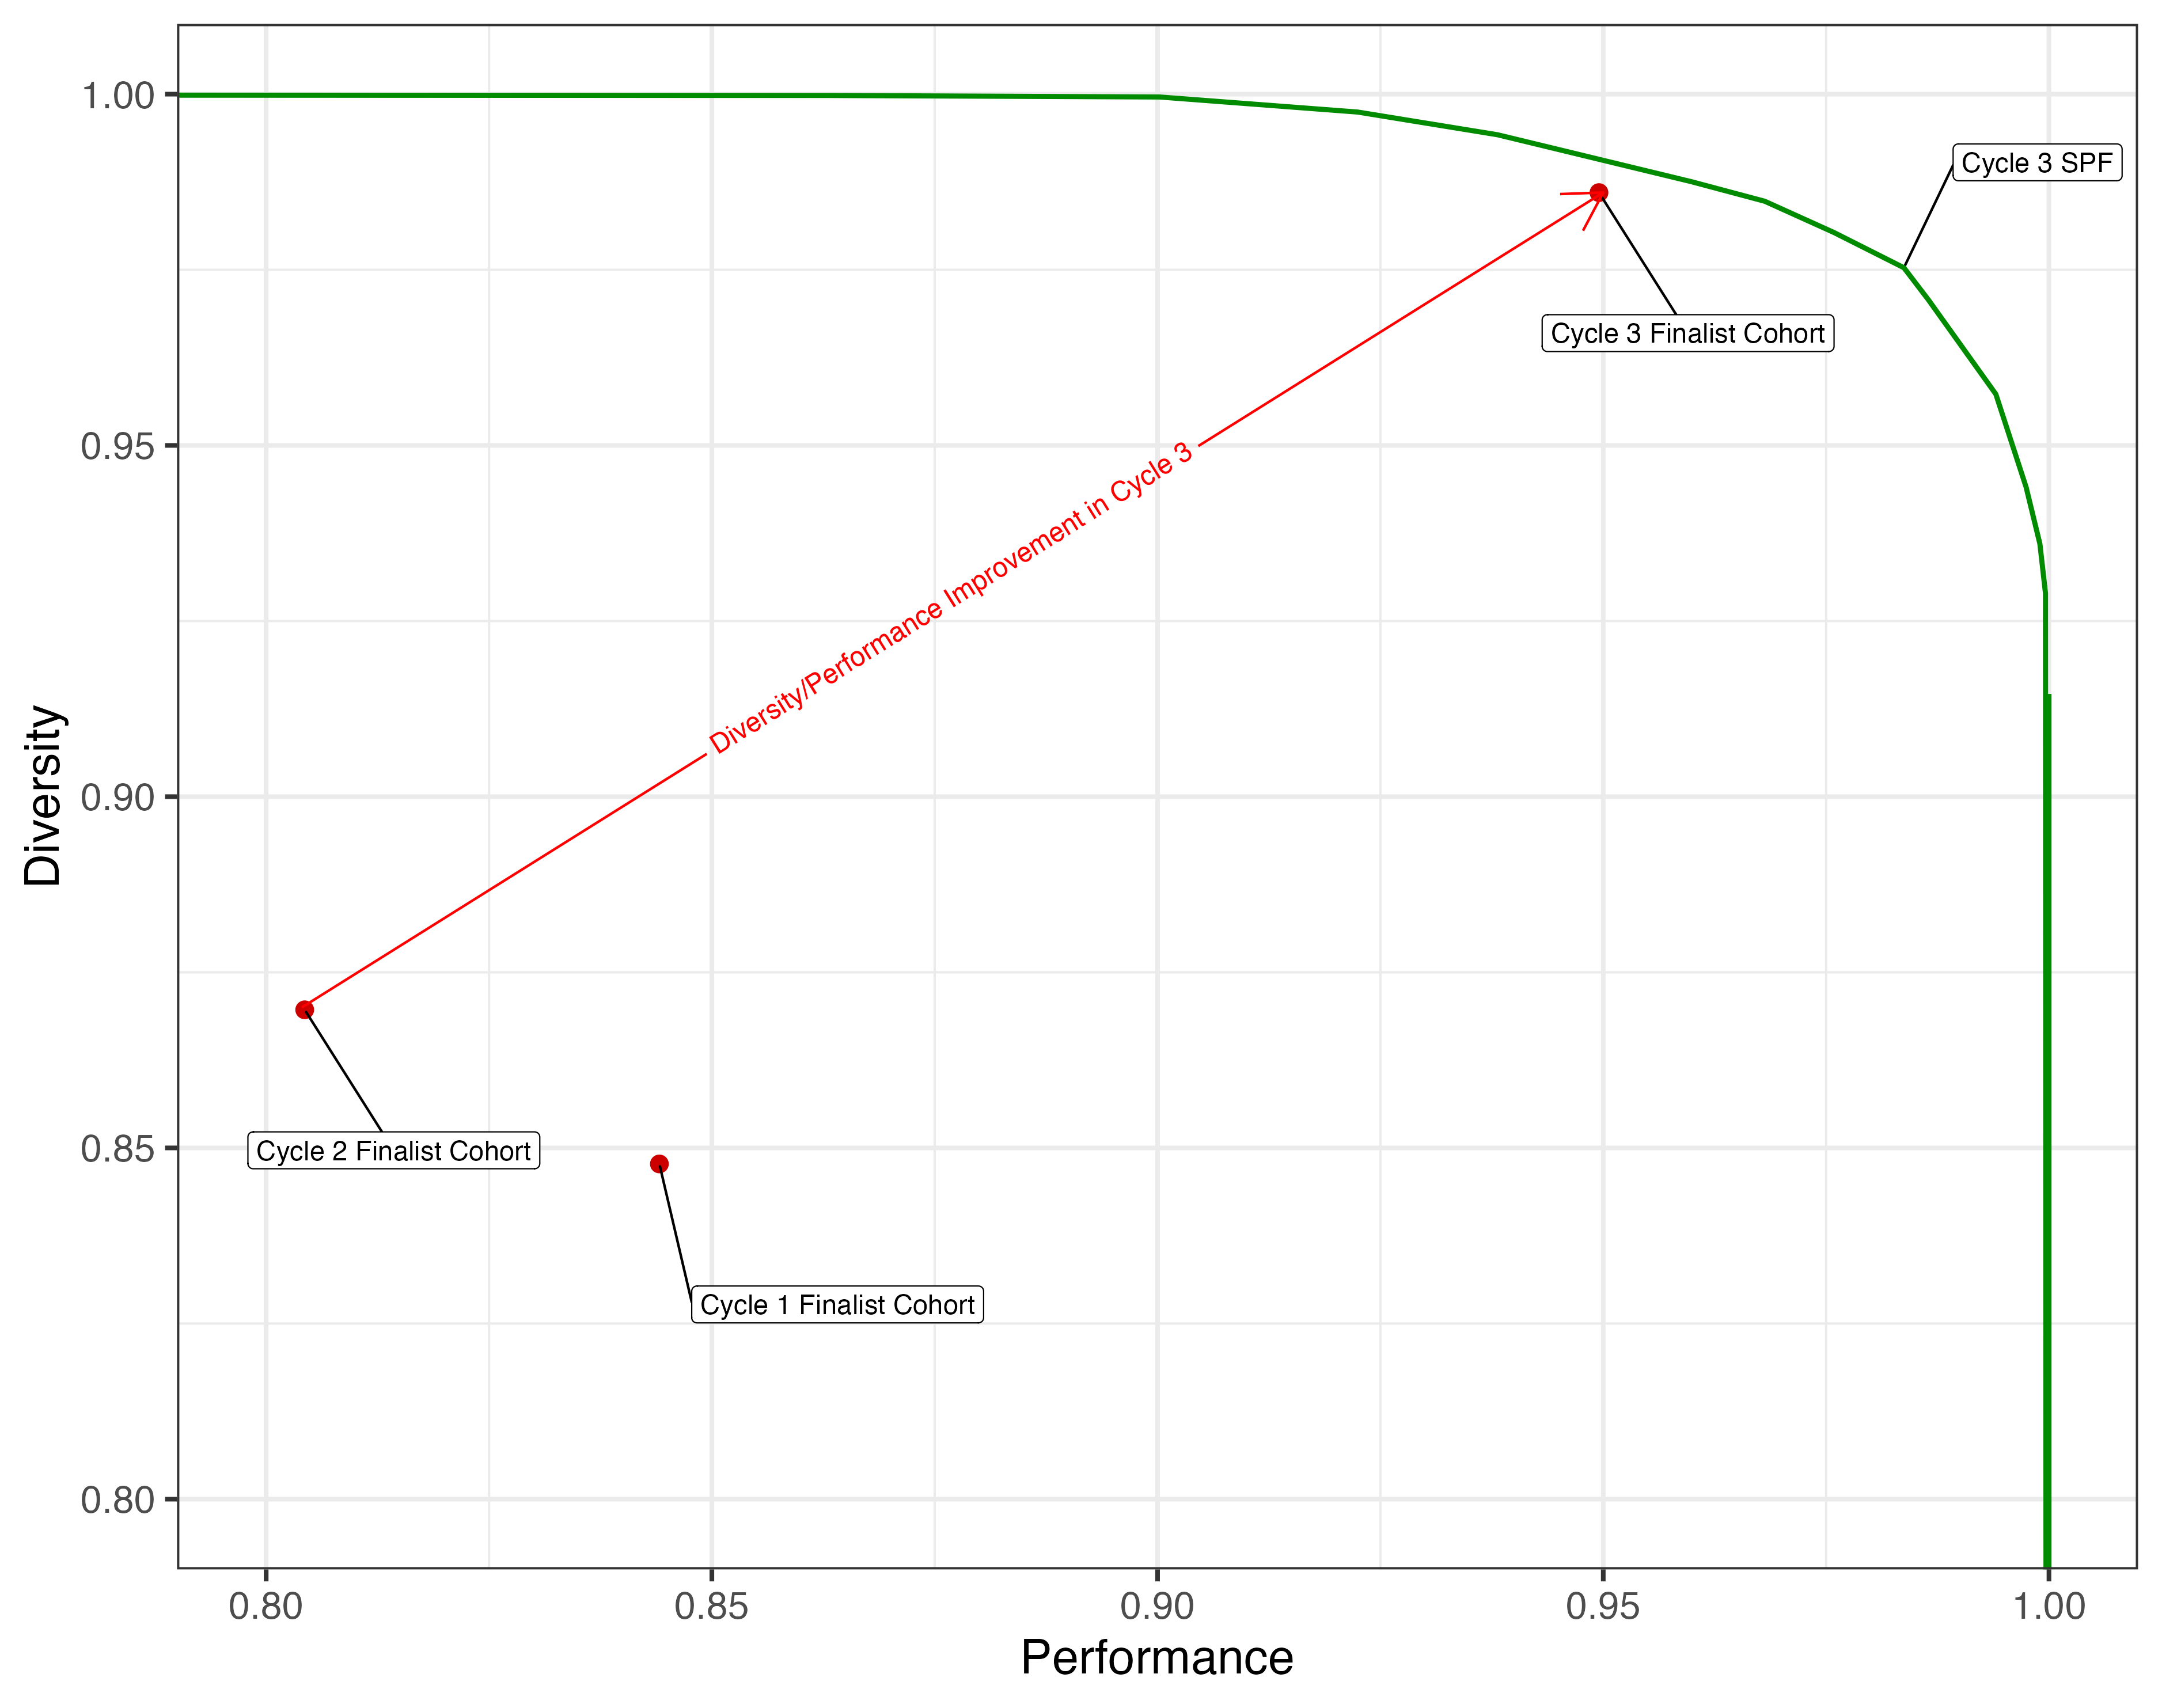
\includegraphics[width=\textwidth,height=\textheight,keepaspectratio]{spf/yr3_spf_finalist.png} 
%     \end{figure}
    
    
%     \newpage
%     \begin{figure}[!htb]
%     \centering
%         \caption{This figure displays permutations tests of the distributions of differences in project performance (panel a) and diversity (panel b) from 1000 randomly drawn pairs of potential cohorts from application cycle 1. The dashed black vertical line represents the 95 percentile of these differences. The solid vertical lines represent the max pareto gain on performance (panel a) and diversity (panel b) in each application year.} \label{fig:permutation_tests}
%       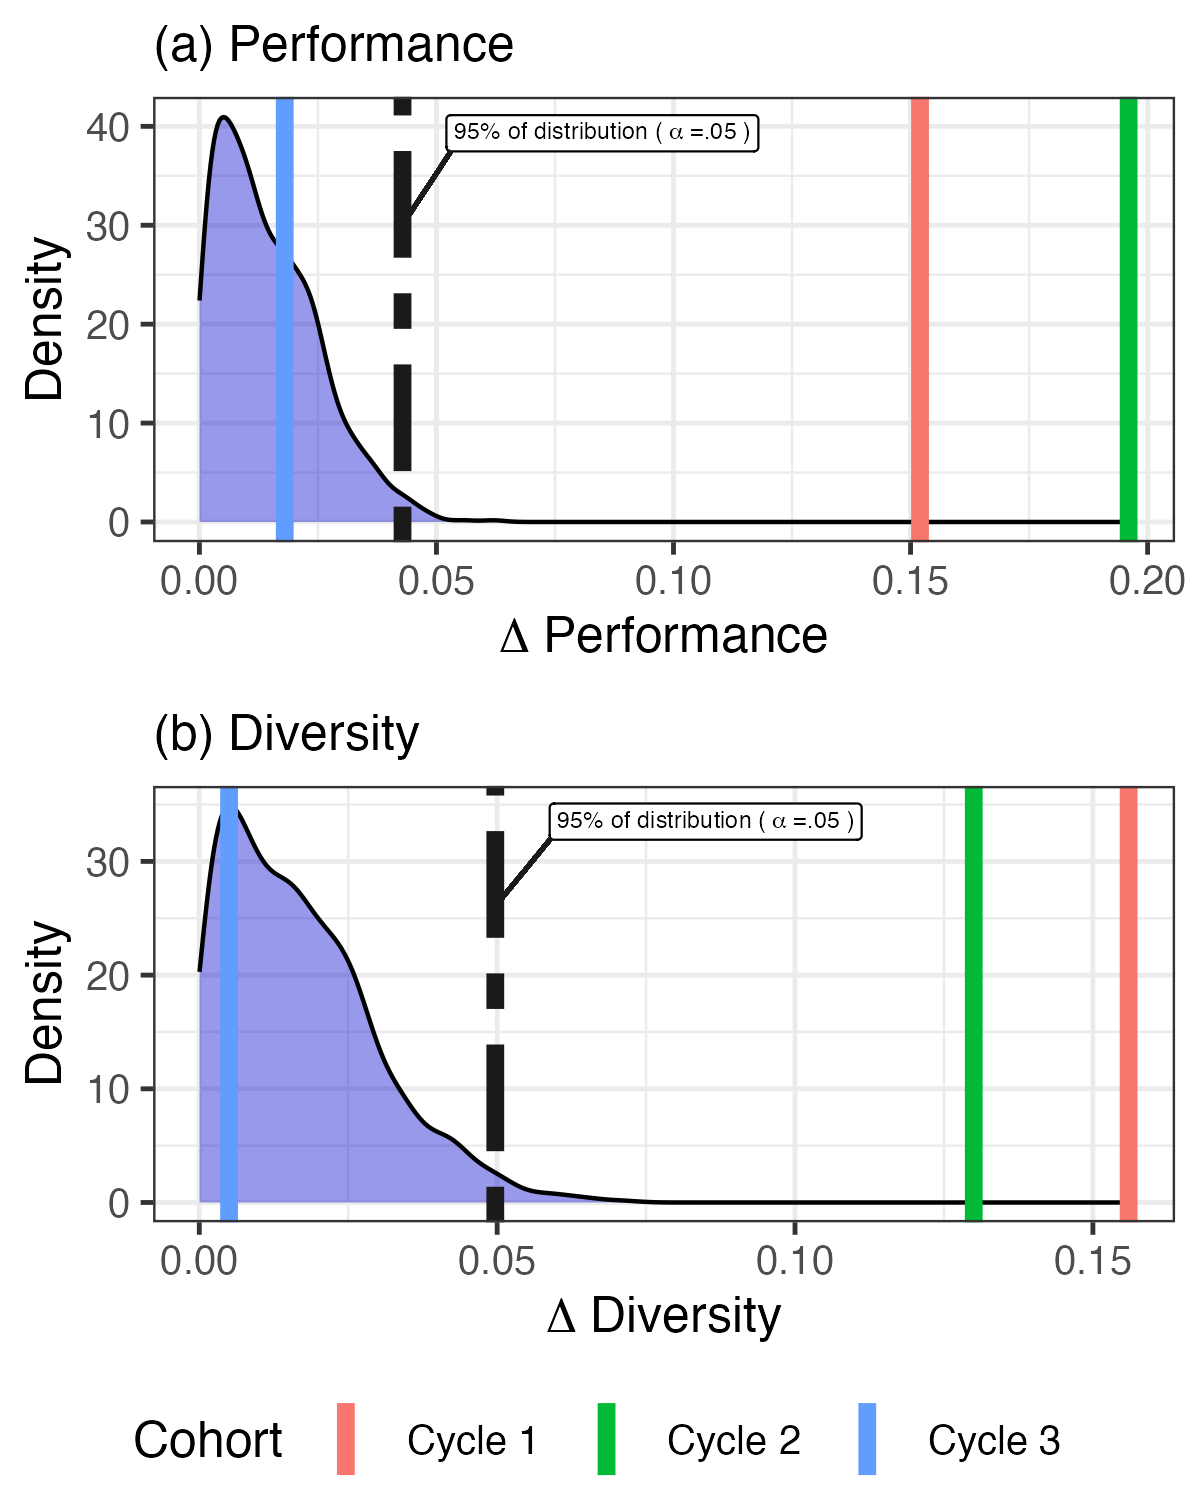
\includegraphics[width=.9\textwidth,height=\textheight,keepaspectratio]{spf/permutation_tests.png} 
%     \end{figure}
    
%     \newpage
%     \begin{figure}[!htb]
%     \centering
%         \caption{This figure plots the percentile of average expert-judged project quality (i.e. performance) by deciles of cognitive, peer, and traditional scores for the Cycle 2021 cohort. The cognitive score is the percentile of the candidate's IQ, the peer score is the percentile of the average peer assessment of each applicant video, and the traditional score is the average percentile of a candidate's IQ and project essay rating.   } \label{fig:alt_talent_dist}
%       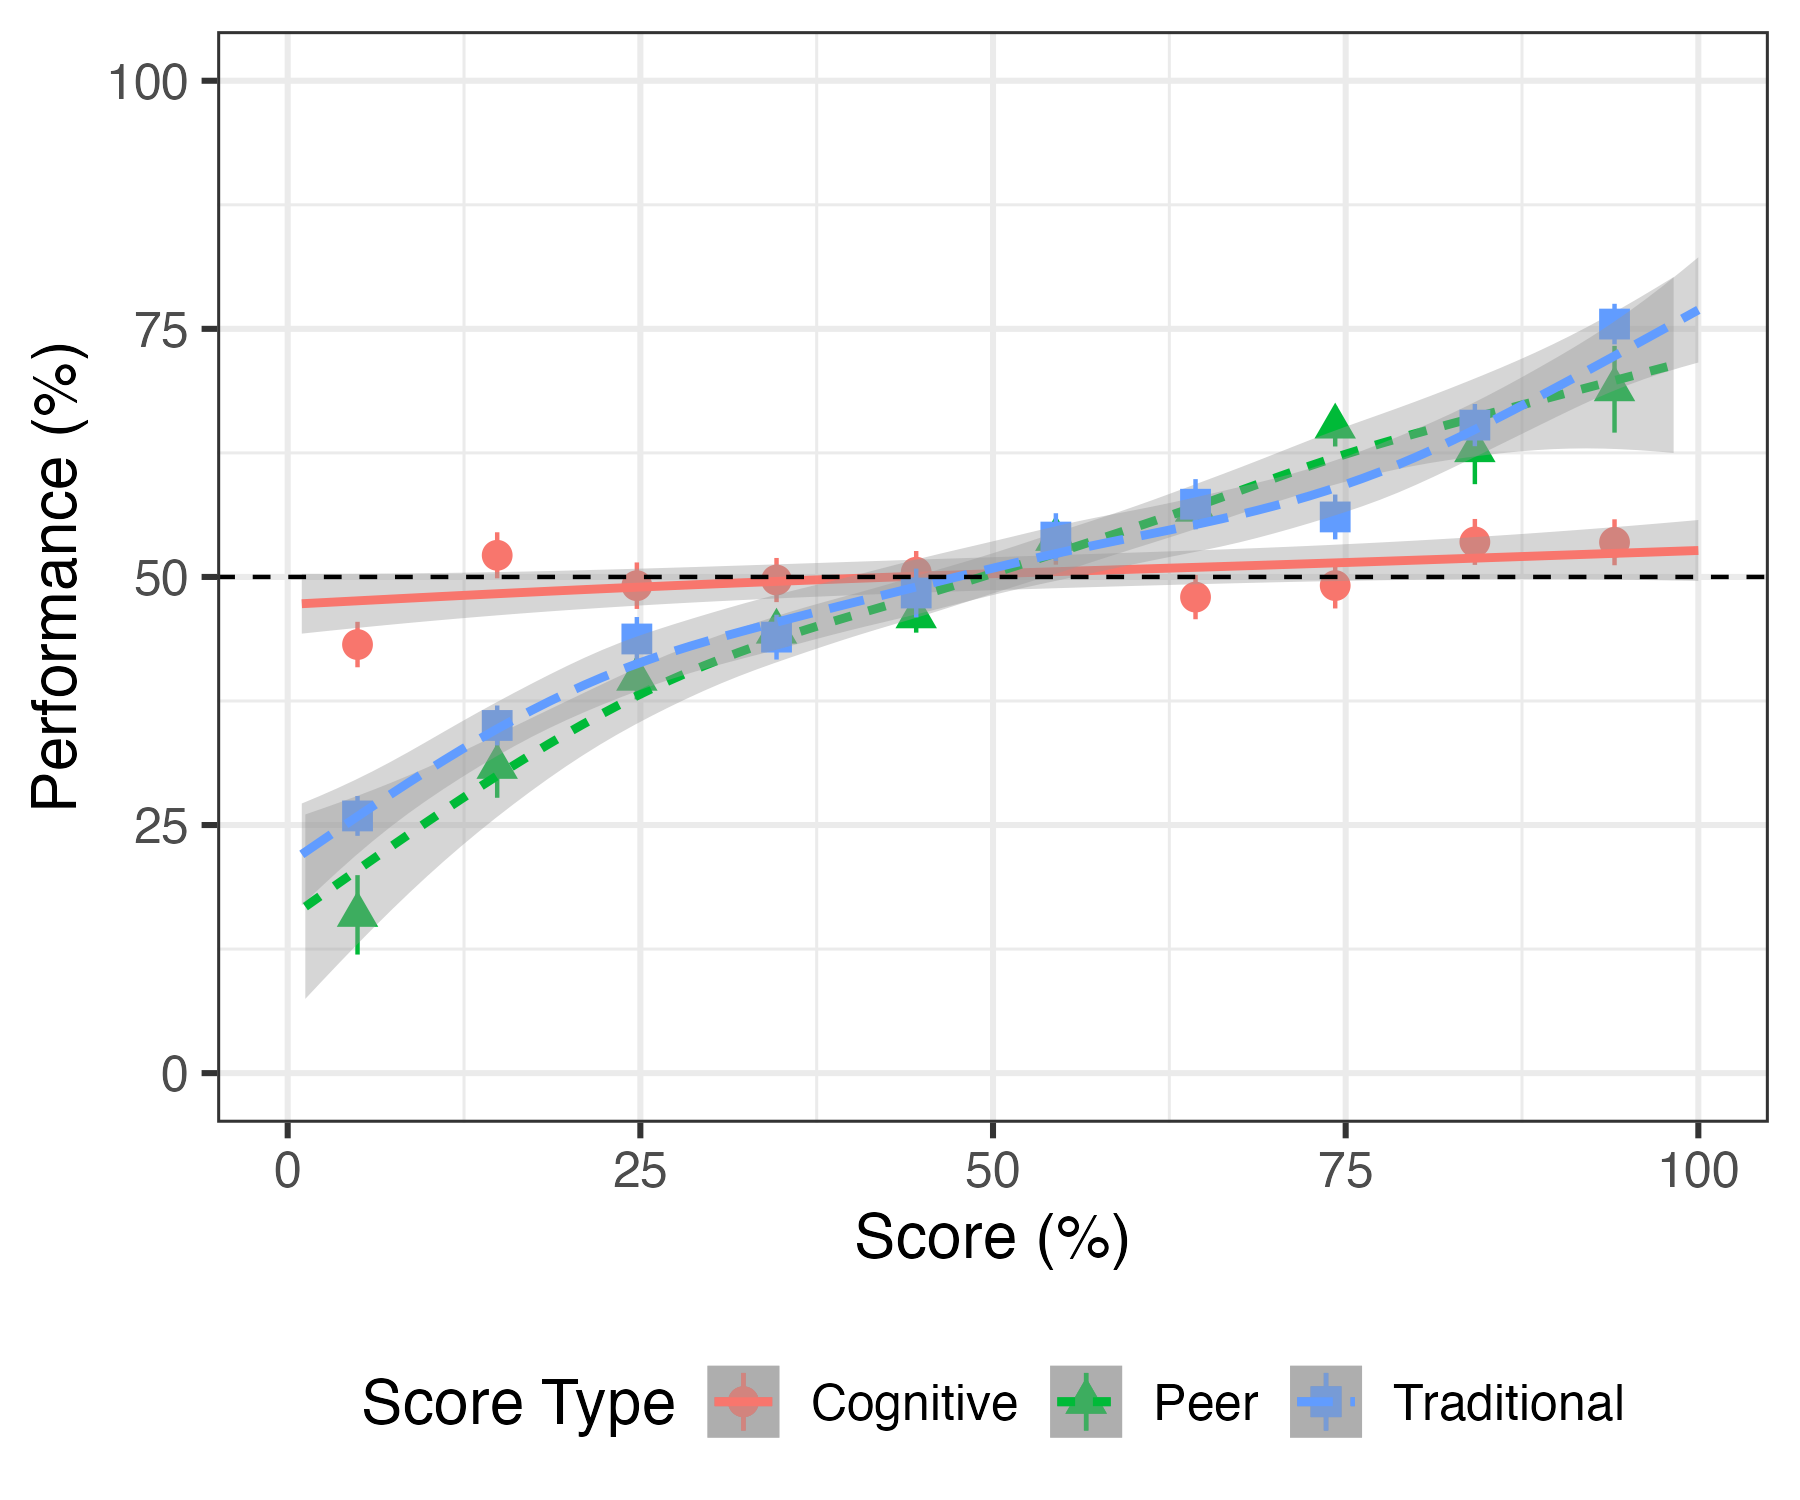
\includegraphics[width=\textwidth,height=\textheight,keepaspectratio]{spf/pq_by_scores_c1.png} 
%     \end{figure}
    
%     \newpage
%     \begin{figure}[!htb]
%     \centering
%         \caption{This figure plots the average of various measures of applicant socioeconomic (dis)advantage by deciles of cognitive, peer, and traditional scores for the cycle 1 cohort. The measures of (dis)advantage from Panel A to D in order are predicted mean parent income (yearly), years of education of most educated parent, whether or not the applicant lives in a globally poor household (mean parent income less than \$1,000 a year), and whether or not the applicant lives in a poor country (less than \$12,000 GDP per capita). The cognitive score is the percentile of the candidate's IQ, the peer score is the percentile of the average peer assessment of each applicant video, and the traditional score is the average percentile of a candidate's IQ and project essay rating.  } \label{fig:disadvantage_corr}
%       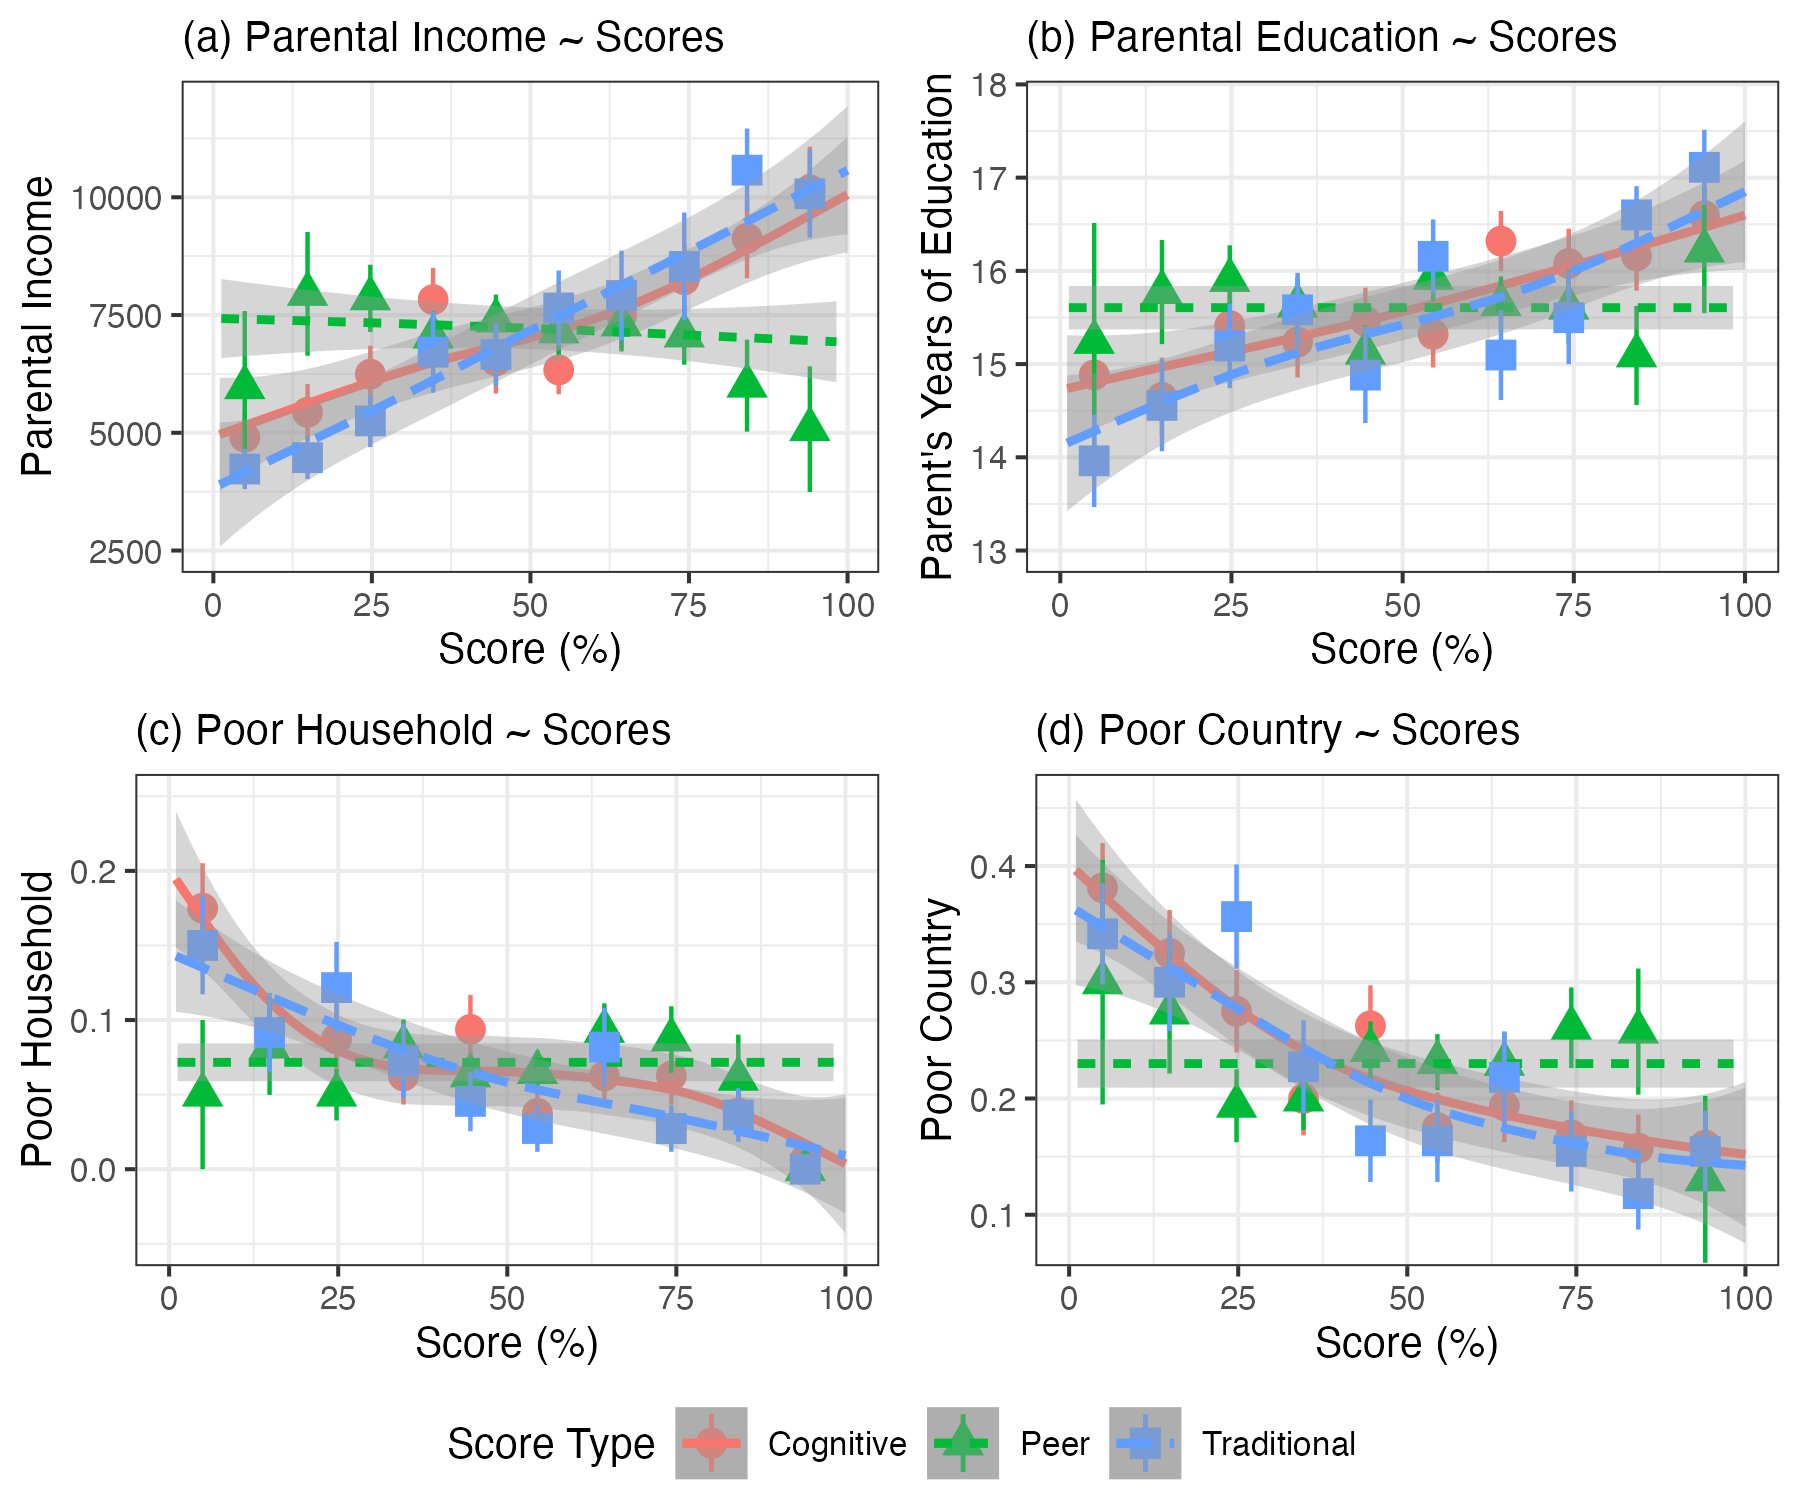
\includegraphics[width=\textwidth,height=\textheight,keepaspectratio]{spf/disadvantage_by_scores.png} 
%     \end{figure}
    
%     \newpage
%     \begin{figure}[!htb]
%     \centering
%         \caption{This figure displays various SPF estimates for the  finalist cohort using the program's notion of diversity (Panel a), a disadvantage notion of diversity (Panel b), and a representativeness notion of diversity (Panel c). The y-axes represent diversity scores while the x-axes represent average cohort performance (i.e. project scores). The green curves are our estimates of three alternative cycle 1 SPFs, which are estimates the upper bound of diversity that is achievable at every level of cohort performance. Each dot represents the performance and diversity of cohorts had they been selected using those with the highest cognitive (blue), traditional (green), or peer (red) scores.  Each dot represents the performance and diversity of cohorts had they been selected using only cognitive ability (blue), a combination of written essay judgements and cognitive ability (aka a "traditional" score, which is green), and just peer review (red).} \label{fig:alt_screen}
%       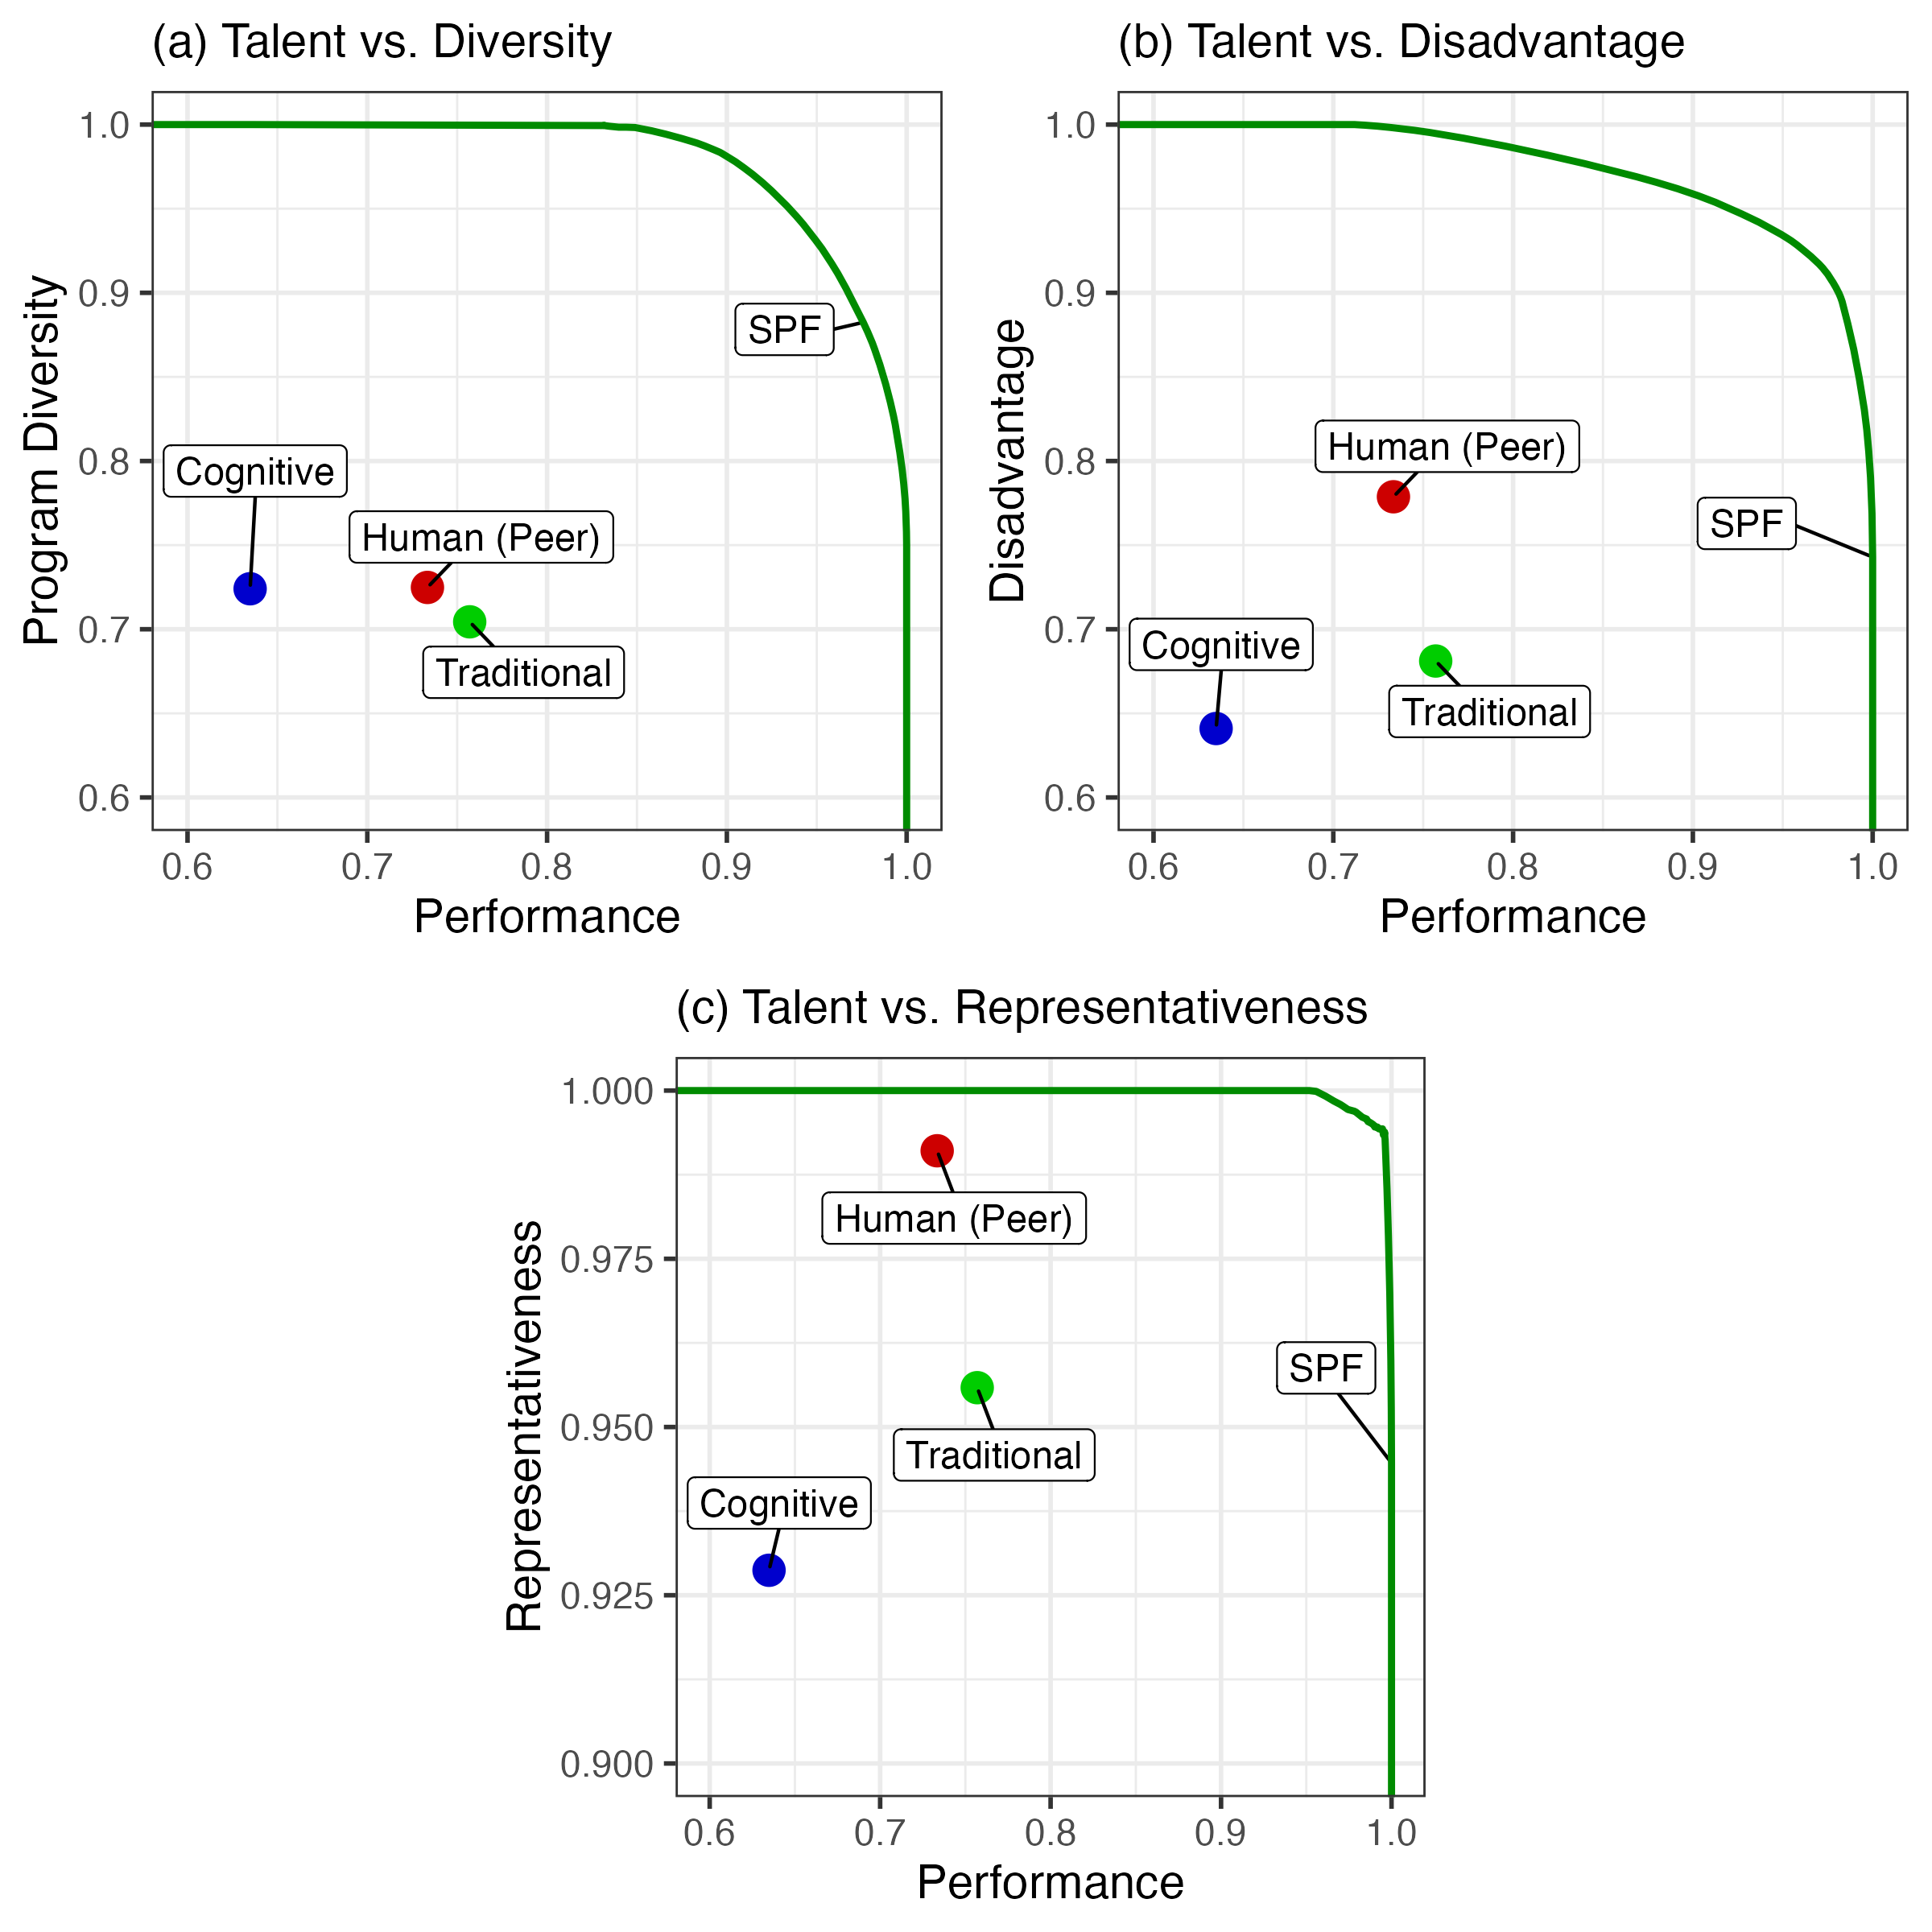
\includegraphics[width=\textwidth,height=\textheight,keepaspectratio]{spf/alt_screening_performance.png} 
%     \end{figure}
    
%     \newpage
%     \begin{figure}[!htb]
%     \centering
%         \caption{This figure displays the SPF we estimated for the cycle 1 finalist cohort and an SPF based on a more traditional method of measuring performance (i.e. the average of cognitive ability and an essay assessment). The y-axis represents the diversity score while the x-axis represents average cohort performance on projects or the traditional score. The vertical distance between the SPFs represents the difference in maximal diversity conditional on a cohort performing at a particular percentile of both scores. } \label{fig:compare_div_tradeoffs}
%       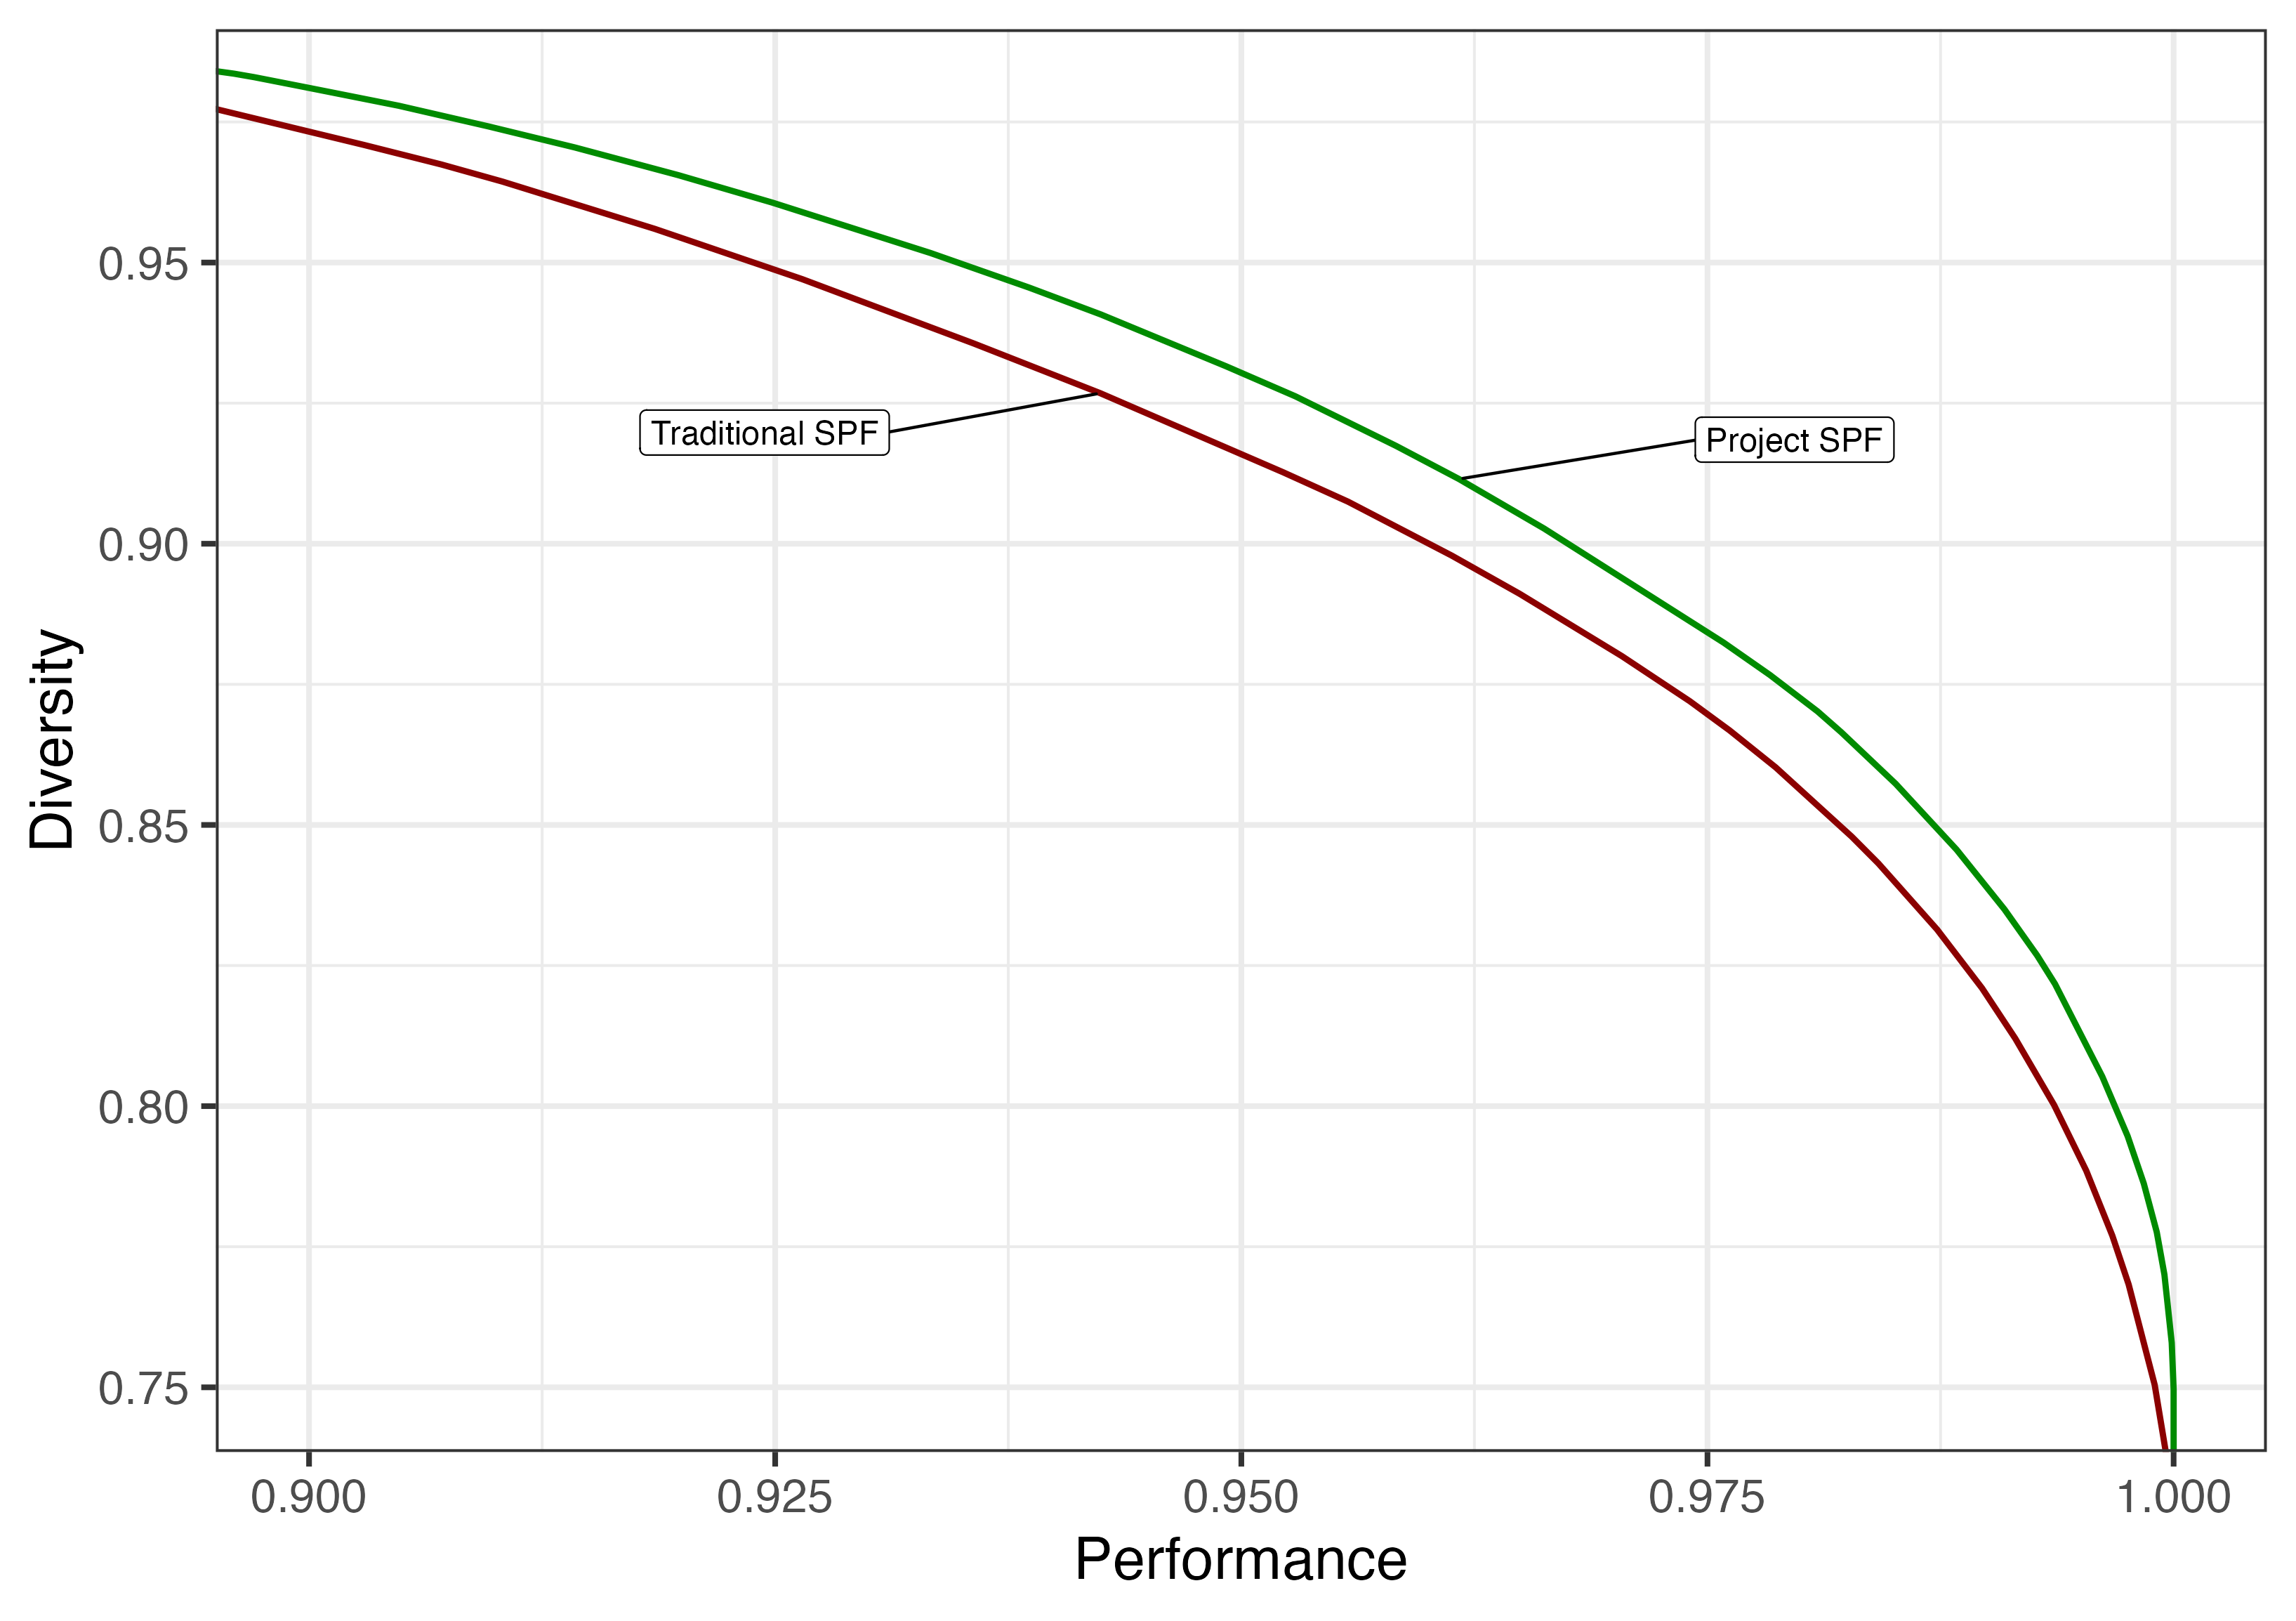
\includegraphics[width=\textwidth,height=\textheight,keepaspectratio]{spf/alt_merit_spfs.png} 
%     \end{figure}
    
%     \newpage
    
% \begin{table}[htbp] 
%     \centering 
%     \caption{Summary Statistics:  Risepplicants. Raw data come from surveys completed by applicants. Data are pooled across three application years.}
%     \label{tab:pooled_demo}
%     \begin{tabular}{@{\extracolsep{5pt}}lccccc} 
%     \\[-1.8ex]\hline 
%     \hline \\[-1.8ex] 
%     \emph{Panel A: Demographics} & \multicolumn{1}{c}{N} & \multicolumn{1}{c}{Mean} & \multicolumn{1}{c}{St. Dev.} & \multicolumn{1}{c}{Min} & \multicolumn{1}{c}{Max} \\ 
%     \hline \\[-1.8ex] 
%     Male & 5,772 & 0.41 & 0.49 & 0 & 1 \\ 
%     Age & 5,770 & 16.43 & 0.81 & 15 & 18 \\ 
%     Poor Country & 5,720 & 0.42 & 0.49 & 0 & 1 \\ 
%     Poor Household & 5,772 & 0.18 & 0.38 & 0 & 1 \\ 
%     Yrs of Parent Education & 5,772 & 15.21 & 4.45 & 0 & 20 \\ 
%     Mean Parent Income (\$) & 5,772 & 18,891 & 39,617 & 227 & 250,000 \\ 
%     \hline
%     & & & & & \\
%     \emph{Panel B: Global Region} & \multicolumn{1}{c}{N} & \multicolumn{1}{c}{Mean} & \multicolumn{1}{c}{St. Dev.} & \multicolumn{1}{c}{Min} & \multicolumn{1}{c}{Max} \\ 
%     \hline
%     Latin America & 5,770 & 0.25 & 0.43 & 0 & 1 \\ 
%     Sub-Saharan Africa & 5,770 & 0.20 & 0.40 & 0 & 1 \\ 
%     Middle East & 5,770 & 0.18 & 0.38 & 0 & 1 \\ 
%     Canada/US/UK+ & 5,770 & 0.14 & 0.35 & 0 & 1 \\ 
%     India & 5,770 & 0.08 & 0.27 & 0 & 1 \\ 
%     East Asia & 5,770 & 0.06 & 0.23 & 0 & 1 \\ 
%     Western Europe & 5,770 & 0.04 & 0.20 & 0 & 1 \\ 
%     Eastern Europe & 5,770 & 0.04 & 0.20 & 0 & 1 \\ 
%     Caribbean/Pacific Islands & 5,770 & 0.01 & 0.08 & 0 & 1 \\ 
%     \hline \hline \\[-1.8ex] 
%     \end{tabular} 
%     \end{table} 
    
%     \newpage
%     \begin{table}[!htbp] \centering 
%       \caption{Summary Statistics: Project Reviewers. Raw data come from surveys completed by applicants. Data are pooled across three application years.}\label{tab:pooled_rev_demo}
%       \label{} 
%     \begin{tabular}{@{\extracolsep{5pt}}lccccc} 
%     \\[-1.8ex]\hline 
%     \hline \\[-1.8ex] 
%     \emph{Panel A: Demographics} & \multicolumn{1}{c}{N} & \multicolumn{1}{c}{Mean} & \multicolumn{1}{c}{St. Dev.} & \multicolumn{1}{c}{Min} & \multicolumn{1}{c}{Max} \\ 
%     \hline \\[-1.8ex] 
%     Male & 1,290 & 0.43 & 0.50 & 0 & 1 \\ 
%     Age & 1,309 & 44.50 & 19.99 & 19 & 75 \\ 
%     Poor Country & 1,321 & 0.46 & 0.50 & 0 & 1 \\ 
%     \hline
%     & & & & & \\
%     \emph{Panel B: Global Region} & \multicolumn{1}{c}{N} & \multicolumn{1}{c}{Mean} & \multicolumn{1}{c}{St. Dev.} & \multicolumn{1}{c}{Min} & \multicolumn{1}{c}{Max} \\ 
%     \hline
%     Canada/US/UK+ & 1,334 & 0.37 & 0.48 & 0 & 1 \\ 
%     India & 1,334 & 0.28 & 0.45 & 0 & 1 \\ 
%     Western Europe & 1,334 & 0.07 & 0.25 & 0 & 1 \\ 
%     Middle East & 1,334 & 0.07 & 0.26 & 0 & 1 \\ 
%     Sub-Saharan Africa & 1,334 & 0.06 & 0.24 & 0 & 1 \\ 
%     Latin America & 1,334 & 0.06 & 0.24 & 0 & 1 \\ 
%     East Asia & 1,334 & 0.06 & 0.24 & 0 & 1 \\ 
%     Eastern Europe & 1,334 & 0.01 & 0.12 & 0 & 1 \\ 
%     Caribbean/Pacific Islands & 1,334 & 0.004 & 0.07 & 0 & 1 \\ 
%     \hline \hline \\[-1.8ex] 
%     \end{tabular} 
%     \end{table} 